%\documentclass[a4paper,twoside,12pt,dvipdfm]{report}
\documentclass[11pt, a4paper]{report}

%\usepackage [shownotes,demo]{101labs}
\usepackage{101labs}

\addbibresource{101labs.bib}
\addbibresource{latex-exercise.bib}

\coursecode{COMP10120}
\coursename{Introductory Labs}
\title{Lab exercises}
\date{August 2013}
\author{Steve Pettifer, Toby Howard, Graham Gough and John Latham}
\bottomstuff{\noindent
\includegraphics[width=2cm]{images/rpi-logo}\hspace*{\fill}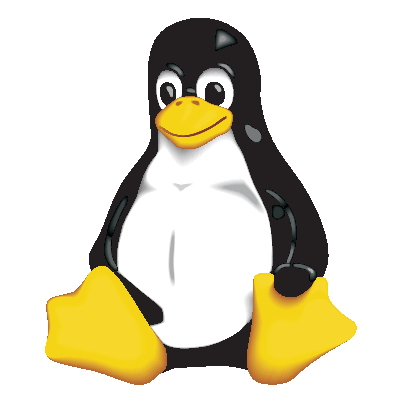
\includegraphics[width=2cm]{images/Tux}}

\mkcmdanchor{echo}{Miscellaneous}
\mkcmdanchor{ls}{File_System_Utilities} 
\mkcmdanchor{mkdir}{File_System_Utilities} 
\mkcmdanchor{cd}{File_System_Utilities} 
\mkcmdanchor{pwd}{File_System_Utilities}  
\mkcmdanchor{rm}{File_System_Utilities}   
\mkcmdanchor{mv}{File_System_Utilities}    
\mkcmdanchor{which}{Finding_Files}    
\mkcmdanchor{gzip}{File_Compression}
\mkcmdanchor{zip}{File_Compression}
\mkcmdanchor{tar}{File_Compression}
\mkcmdanchor{man}{Getting_Help}
\mkcmdanchor{less}{File_Viewing}
\mkcmdanchor{more}{File_Viewing}
\mkcmdanchor{cat}{File_Viewing}
\mkcmdanchor{head}{File_Viewing}
\mkcmdanchor{tail}{File_Viewing}

  \dominitoc
 
  \includeonly{rpi1}

  
\begin{document}

\maketitle
\firstcommand{\tableofcontents\clearpage}


%%% Local Variables: 
%%% mode: latex
%%% End: 

\coursecode{Welcome}
\setcounter{chapter}{-1}
\renewcommand{\chaptername}{Welcome Lab Session}
\setcounter{chapter}{-1}
\newcommand{\splunge}{\textcolor{red}{\bf SPLUNGE}}

\chapter{Getting started}
\label{cha:getting-started}

\minitoc

\section{Welcome}


Hello and welcome. In this first, introductory, lab we're going to
cover some of the basic things you'll need to know about the IT
infrastructure here in the School of Computer Science. Some of what we
tell you may well seem very obvious to you, and if that's the case
we'd ask you to be patient. Some other things might not be so obvious...

In this and every lab there will be academic staff and postgraduate students (demonstrators) around to help you. If you're stuck or find something that you really can't understand, then \emph{please ask for help}; that's what the lab staff are here for, don't just sit there getting frustrated.

All the desktop PCs in the labs in the Kilburn building are
`dual-boot': they can be started up running either Linux or
Windows. This is for flexibility -- the labs for most course units  use
Linux, but some use Windows, and of course, outside the labs, you're free to use
whichever you prefer for any aspect of your studies. If you're not
familiar with Linux, don't worry. We'll be telling you a bit about it
in this lab, and you'll be looking at it in much more detail in subsequent labs.

\section{Using Windows}
\label{sec:using-windows}

We'll start with Windows, so the first thing we need to do is to make
sure your PC is running Windows. Have a look. If it is, 
and the screen looks like Figure~\ref{figure:welc-screen}, then you  you can move on to the end of this subsection and login.

If it's currently in Linux, showing a black screen with a login prompt,  you need to reboot the PC. To do
this, press \ttout{ctrl}, \ttout{alt} and \ttout{delete}.

This will probably cause strange messages to appear on the screen,
disappear, and be replaced by yet more strange messages. Be patient,
watch it all happen, and don't worry what it all means. After a while,
everything should settle down and the screen will look like
Figure~\ref{figure:welc-grub}.

\begin{figure}
\centerline{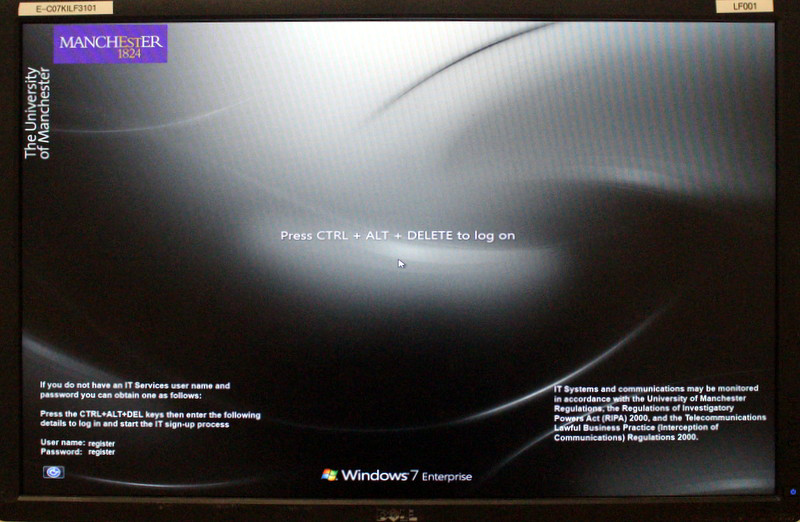
\includegraphics[width=15cm]{images/TH-win-welcome}}
\caption{The Windows7 Welcome screen.}
\label{figure:welc-screen}
\end{figure}

\begin{figure}
\centerline{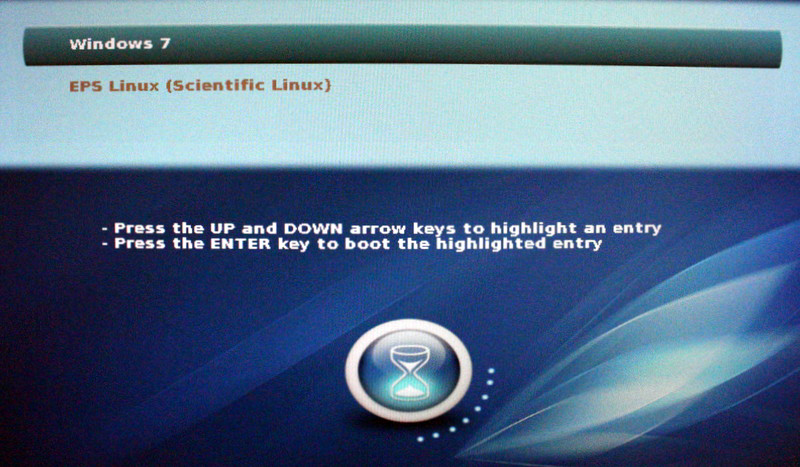
\includegraphics[width=15cm]{images/TH-grub-win}}
\caption{The boot selection menu screen.}
\label{figure:welc-grub}
\end{figure}

This is where you decide whether to start up Windows or Linux. If you do nothing, this will automatically boot into the default operating system after a fixed timeout period. In order to stop this timeout process, just press the space bar (or any other key). Now use the
up/down arrow keys on the keyboard to highlight the line
reading \ttout{Windows 7}, and press the enter key. After a short while, the Windows 7
welcome screen will appear, as shown in Figure~\ref{figure:welc-screen}. Now use the ctrl-alt-del chord again as instructed and you should see the Windows 7 login screen, as shown in Figure~\ref{figure:login-screen}.

\begin{figure}
\centerline{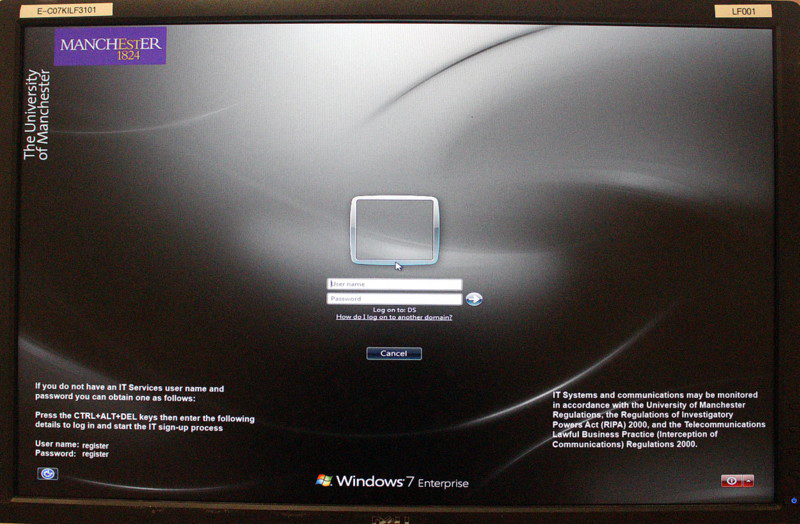
\includegraphics[width=15cm]{images/TH-win-login}}
\caption{The Windows 7 login screen.}
\label{figure:login-screen}
\end{figure}

To log in to your personal account, type in your username (this is an
8-character name starting with an `m' that you were given at registration). Your password will
be the one  you set at registration. If your password doesn't work, or if you've forgotten it,
you need to fix this urgently. You can:

\begin{itemize}
  \item On a machine running Windows, login with the username \ttout{register} and password \ttout{register}, then follow the instructions.
\item If you have access to a web browser, use the password recovery page at\\ \url{https://iam.manchester.ac.uk/recovery_login/overview}
%\item Visit the \verb|it.changes| Helpdesk in Kilburn Lower First area (Welcome Week, 09:00 -- 17:00)
\item Outside lab times, you can contact the University IT helpdesk (opening hours are Monday to Friday 9am to 5pm.) by phone on 0161 306 5544, or dial 65544 from a University internal phone; or you can visit the helpdesk in John Rylands Library (Building 55 on
the Campus Map), at the top of the escalator in the Blue 1 area.
\item Remember, if you need help, ask!
\end{itemize}

Once you're logged in, go to your MyManchester page in a web browser, at

\url{https://my.manchester.ac.uk}

This page should look something like Figure~\ref{figure:welc-mymanchester}.

\subsection{Reading your email}

We use email extensively in the School, so it's vitally important that
you read your mail regularly -- at least once a day (and probably much
more often!). Follow the mail link (indicated by the green arrow in
Figure~\ref{figure:welc-mymanchester}) to access your email on the
University's Office365 system. This is a fully-featured system that
gives you 25GB of email storage space and an integrated calendar. You should
see a page looking something like Figure~\ref{figure:welc-mail365}.

Have a look around for a few minutes and check what mail you've
got. In particular, look for one with ``The Monday Mail'' in the
Subject line. This an important mail you'll receive every Monday
(hence the name) throughout your 3 or 4 years with us in the
School. The Monday Mail tells you what's going on each week in the
School. Take a moment to read it now. You can always read the Monday Mail, by the way, at the archive located at\\  \urlnop{studentnet.cs.manchester.ac.uk/ugt/mondaymail/}

\begin{figure}
\centerline{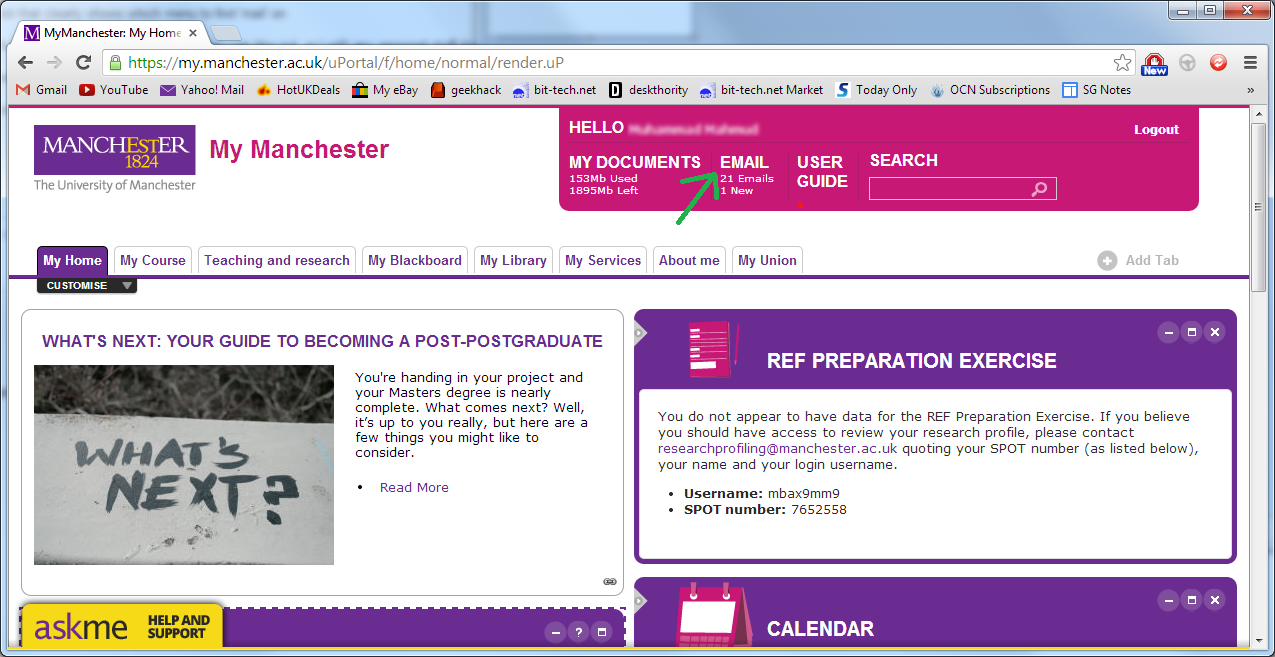
\includegraphics[width=15cm]{images/hamza-email-link.png}}
\caption{Your MyManchester page.}
\label{figure:welc-mymanchester}
\end{figure}

\begin{figure}
\centerline{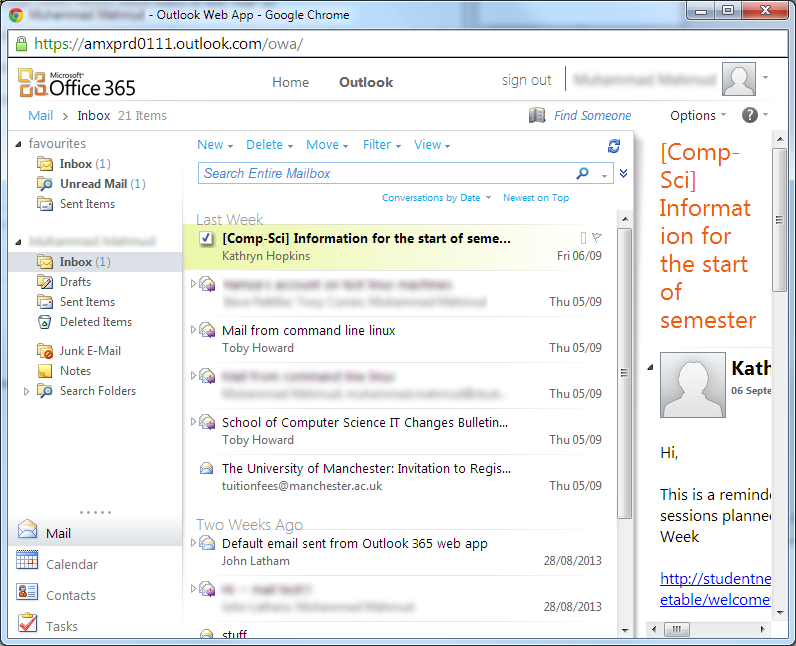
\includegraphics[width=15cm]{images/hamza-365-mail.png}}
\caption{Your Office365 email.}
\label{figure:welc-mail365}
\end{figure}

\label{sec:reading-your-mail}

Office365, like most modern email systems, supports the IMAP
protocol -- which means that you can access your mail from any device
that can run an IMAP mail client. Some examples of such clients are:
Mozilla Thunderbird, Mac Mail, Windows Live Mail and mail apps on mobile devices. No matter what
client you use, you need to tell it the appropriate settings. The mechanism for finding these setting can be found in our student wiki, which is located on the web at \urlnop{wiki.manchester.ac.uk/compsci/index.php/It.changes}. Look for the answer to question 'How do I configure my favourite IMAP mail client?'. This wiki provides help about the major changes we have made to our IT infrastructure this summer; there is also a general FAQ at \urlnop{wiki.manchester.ac.uk/compsci/index.php/StudentFAQ}. Please make use of these useful sources of information.

Once you've found the settings, use Office365 to email this information to yourself, to your
University account:

\url{firstname.lastname@student.manchester.ac.uk}

You'll need this information in a later lab so please don't delete this email after you've read it.

Finally, if you use an IMAP mail client on your phone or mobile
device, configure it to use the settings you've just found, and check
that you can read and send email successfully.

That's all on Windows for now, but of course  you're free to boot an available PC into Windows  and use it at any time unless you are in a lab that requires the use of Linux. Next, we're going to take a first look at Linux.

\subsection{Rebooting into Linux}
\label{sec:rebooting-into-linux}

So let's reboot the PC, and start it up in Linux. First, log out of
Windows by selecting the Windows icon in bottom left and then \ttout{Log off}). Get back to the login screen, click the
small icon in the lower right of the screen (see Figure~\ref{figure:welc-restart}) and select \ttout{Restart}.

\begin{figure}
\centerline{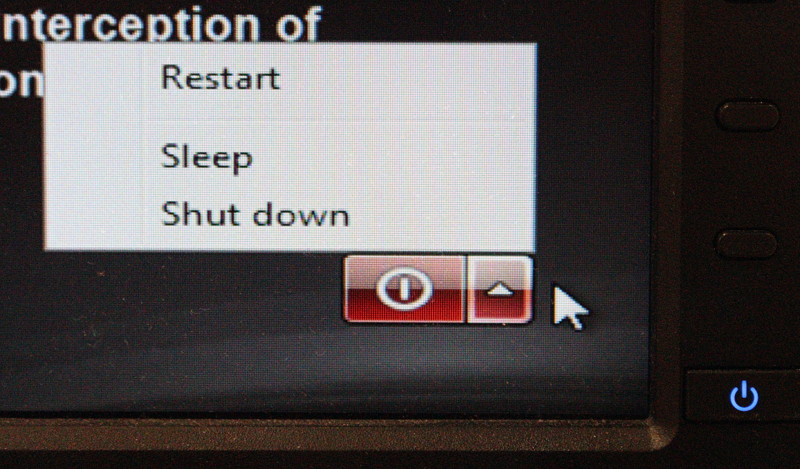
\includegraphics[width=0.4\textwidth]{images/TH-shutdown-win}}
\caption{Restarting the PC.}
\label{figure:welc-restart}
\end{figure}

The system will shut down and we'll be back to the boot selection menu
screen we saw earlier in Figure~\ref{figure:welc-grub}. This time, use
the up/down arrow keys to select \ttout{EPS Linux (Scientific
  Linux)}. Linux will now start, and after a short while you should
see a black screen, with a white login prompt. We won't login to Linux
at this stage, that can wait until a later lab, next week. We would,
however, like you to read the rest of this document, which gives you
some useful and interesting background information about Linux. If you
don't have time to finish reading it in the lab, please make sure you
do so before the next lab session.

%\section{Using the School Linux system}
\section{Unix and Linux}

Over the next couple of weeks you will be undertaking a number of
introductory labs to familiarise yourself with the School's computing
infrastructure. Much of this is based on devices and machines running Linux, a
variant of the Unix family of operating systems; this document
provides some background on Unix and explains why we think it is
important. It would very useful if you could read this before you
attend the first introductory labs, where the emphasis will be on
leading you through a series of tasks to explore our setup.

\subsection{Operating Systems}

An \wikipedia{Operating_system}{operating system} (OS) is a suite of
software that makes computer hardware usable; it makes the `raw
computing power' of the hardware available to the user. You're
probably most familiar with
the \wikipedia{Microsoft_windows}{Microsoft Windows} and
Apple \wikipedia{OS_X}{OS X} families of operating systems for
`desktop' computers, and \wikipedia{Ios}{iOS} (Apple, again) and
Google's \wikipedia{Android_(operating_system)}{Android} for mobile
devices; but many other more specialist operating systems exist, and
you'll be studying some of these and the principles that underpin OS
design in COMP25111 in your second year. In the meantime, a potted
history of OS development will tide us over\ldots
 
\subsection{Unix Origins}
\label{sec:unix}

In the late 1950s, an American company
called \wikipedia{Bell_Labs}{Bell Laboratories} decided that they
needed a system to improve the way they worked with their computer
hardware (it's probably quite hard to imagine what interacting with a
computer \emph{without} an operating system might be; but it wasn't
pretty and involved manually loading and running programs one by
one). Together with the \wikipedia{General_Electric_Company}{General
Electric Company} and the \wikipedia{MIT}{Massachusetts Institute of
Technology}, they set about the design of an operating system they
called \wikipedia{Multics}{Multics}: the `Multiplexed Information and
Computing Service'. Multics was hugely innovative, and introduced many
concepts that we now take for granted in modern operating systems such
as the ability for more than one program to run `at once'; but it did
rather suffer from `design by committee', and the final system was
seen at the time as being overly complex and rather bloated (`bloated'
is all a matter of perspective of course: its sobering to realise
though that the entire Multics operating system was only around
135Kb. Today's operating systems are something like 30,000 times this
size\ldots). In the late 1960s, a group of programmers at Bell Labs
created a cut-down, leaner and cleaner version of Multics that would
work on more modest hardware. Legend has it that this was to allow
them to play their favourite (only!) computer
game, \wikipedia{Space_Travel_(video_game)}{Space Travel}. In an early
example of the trend of giving things `punny' names, to contrast with
the more clumsy Multics, they called this new system Unix. The
so-called \wikipedia{Jargon_File}{Jargon File} is a good source of
explanations of various bits of computer slang and their obscure
origins, and is well worth a read: in part to give some background
history, but mostly as an insight into the minds of the computing
pioneers of the past!

%\begin{htmlonly}
%(See the Unix entry in the useful and amusing
%\htmladdnormallink{Jargon
%file}{http://www.new.ox.ac.uk/admin/jargon/html/entry/Unix.html}, a
%file}{http://www.cs.manchester.ac.uk/software/jargon/html/entry/Unix.html}, a
%file}{\jargonFileUnix}, a
%`collection of slang terms used by various subcultures of computer
%\htmladdnormallink{hackers}
%{http://www.cs.manchester.ac.uk/software/jargon/html/entry/hacker.html}'.)
%{\jargonFileHackers}'.)
%\end{htmlonly}

Even though Unix is now quite old, most Computer Scientists recognise that the designers of Unix got most of the fundamental concepts and
architecture right. Given how much computing has changed since the 1960s, this was an astonishing intellectual achievement. Although Microsoft's \wikipedia{Microsoft_Windows}{Windows} is by far the most common operating system on \emph{desktop} machines, the majority of the Internet, much of the world's corporate infrastructure, virtually all supercomputers, and even some mobile devices are powered by Unix-like operating systems. So, while the polished graphical user interfaces of Windows and \wikipedia{OS_X}{OS X} appear to dominate the world of computing, most of the real hard-core and leading-edge computation relies on an elegant operating system designed nearly 50 years ago (by a team of scientists who wanted to play a game).  

\subsection{Modern Unix Variants}
\label{sec:modern-unix-variants}


The history of Unix is complex and convoluted, with the system being updated, re-implemented, and mimicked repeatedly over the years, primarily by commercial companies who guarded their versions jealously. Figure \ref{fig:unix-history} shows a tiny fragment of the Unix's `family tree' (the full diagram, which you can find at \urlnop{www.levenez.com/unix/unix.pdf}, is \emph{many} times the size of the portion you can see here).

\begin{figure}[h!tb]
  \begin{center}
    \includegraphics[width=13cm]{images/unix}
  \end{center}
\caption{A fragment of \'{E}ric L\'{e}v\'{e}nez's Unix History chart, reproduced with permission and showing the beginnings of Linux in amongst other versions of Unix.}
\label{fig:unix-history}
\end{figure}
 
Although many of the branches represent interesting innovations of one kind or another, there are perhaps two that deserve particular attention. The first of these was the decision by Apple some time around the turn of the millennium to drop their own---highly popular, but ageing---bespoke operating system (unimaginatively called \wikipedia{Mac_os_9}{Mac OS 9}) in favour of a Unix-based system (now the more familiar `OS X', where `X' is both the Roman numeral `10' and a nod in the direction of the uniX nature of the OS). Although the majority of Mac users are blissfully unaware of the fact, behind the slick front-end of OS X, sits a variant of Unix. The second, and perhaps more profound of these events was the creation in 1991 by Swedish programmer \wikipedia{Linus_torvalds}{Linus Torvalds} of a Unix-like system, the source code to which \emph{he gave away for free}\footnote{`free' here in the sense both of `freedom to reuse or adapt', and also in the sense of `without charge'.}; this became known as the \wikipedia{Linux_kernel}{Linux Kernel}. Combined with other free software created by the \wikipedia{Free_software_foundation}{Free Software Foundation}, a non-commercial version of Unix called \wikipedia{GNU/Linux}{GNU/Linux} was born (GNU here is a recursive acronym for ``GNU's not Unix'', a swipe at other commercial non-Free versions; much to the annoyance of the Free Software Foundation, GNU/Linux is almost always called just `Linux'\footnote{Linux
is pronounced ``Linn-ucks'', despite the fact the name was coined by
its creator, and his name `Linus' is pronounced
``Leen-uss''!}.) 

Linux has been, and continues to be, developed cooperatively by
thousands of programmers across the world contributing their effort
largely free of charge. It is amazing to think that such
a project could ever happen---and it is surely a testament to the
better side of Human nature. But what is interesting is the
observation that these programmers are not motivated by commercial
concerns, but by the desire to make good reliable software and have it
used by lots of people. Thus, Linux is a good choice of Unix: it's
Free, it's efficient, and it's reliable, and it is now used by large corporations, governments, research labs and individuals around the world. Even Google's \wikipedia{Android_(operating_system)}{Android} platform is a Linux-based mobile OS, and the  \wikipedia{Amazon_Kindle}{Amazon Kindle} is also a Linux box behind the electronic ink of its user interface (Figure \ref{fig:kindlelinux}).

\begin{figure}[h!tb]
  \begin{center}
    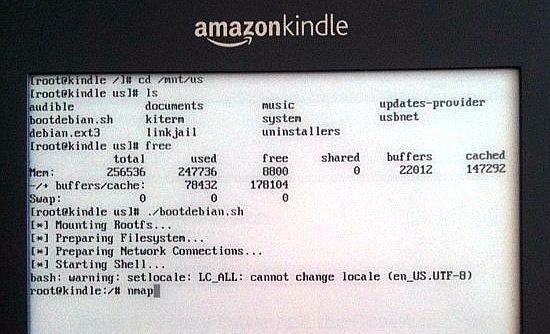
\includegraphics[width=13cm]{images/kindleroot}
  \end{center}
\caption{A photograph of Liraz Siri's `rooted' kindle, showing the Linux command prompt. Reproduced with the author's kind permission from \urlnop{www.turnkeylinux.org/blog/kindle-root}}
\label{fig:kindlelinux}
\end{figure}

One of the results of the fact that Linux is Free is that several
organisations and companies have created their own distributions of
it; these vary a bit (in fact, anybody is free to make any change they
like to Linux, and pass it on to whoever wants it). The distribution
we use in this School is \textbf{Fedora}, which is
one of the most popular and is sponsored by a
US company called \textbf{Red Hat}.
%, which is the latest release

So, if you are to become an expert computer professional, it is
important that you understand the theory and practice of Unix based
systems. Learning Unix is not only a crucial skill for any serious
computer scientist, it is a very rewarding experience; the labs over
the next couple of weeks are designed to help you become familiar with what will be your daily working environment.


\renewcommand{\chaptername}{Intro Lab Session}
\coursecode{Introductory Labs}
` \chapter{Getting started with Raspberry Pi}

% TODO: Intro to what they have been given, and labelling their Pi
% TODO: References, references.
% TODO: Wikipedia links
% TODO: The Pi is yours to keep; if you lose it you'll have to buy another
% TODO: What you'll need to use the Pi at home
% TODO: Where do we introduce 'devices', 'files' and 'processes'? They will see virtual devices like tty0 and sda1 

The Raspberry Pi is an astonishing piece of hardware. Not because it is super-fast or super-powerful---it's actually quite a slow computer by today's standards---but because it is small, cheap and needs very little energy to run. Its cheapness means you can experiment with it safe in the knowledge that if you mess it up, lose it, or drop it into the canal, getting hold of a replacement isn't going to cost you much more than a text-book or a night out at the cinema. Its small size and fairly modest power requirements mean you can be put to use in lots of applications where a regular-sized PC would be impractical.  We hope this will encourage you to experiment and explore, and to take risks playing with both its hardware and software that you might be reluctant to do on your own computer or tablet, or simply can't do with the School's lab machines. 

This lab session is designed to get you familiar with the Raspberry Pi itself, and with some of the basics of the Linux operating system it uses. We're going to be covering a lot of ground quite quickly, and it's important that you read these notes carefully and follow the instructions precisely for now. As the lab sessions progress, the instructions will become much less prescriptive, and we'll be encouraging you to experiment and explore much more, and to find out things for yourself. But for now, just follow our lead. 

Scattered throughout the main text of these exercises there are information boxes of various kinds:
\\

\begin{tabular}{m{1.5cm}m{12cm}}
{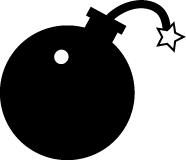
\includegraphics[width=1.5cm]{images/bomb}} & \textbf{Danger!} The bomb icon explains problems and pitfalls, and how to avoid them. It's really important that you read these sections, or you may regret it later.\\
\\

\includegraphics[width=1.5cm]{images/rpi-logo} & \textbf{Raspberry Pi Facts and Factoids.} These sections explain useful but non-essential things about the Raspberry Pi. If you're pushed for time, you can safely skip these boxes and perhaps come back to them another time.\\
\\
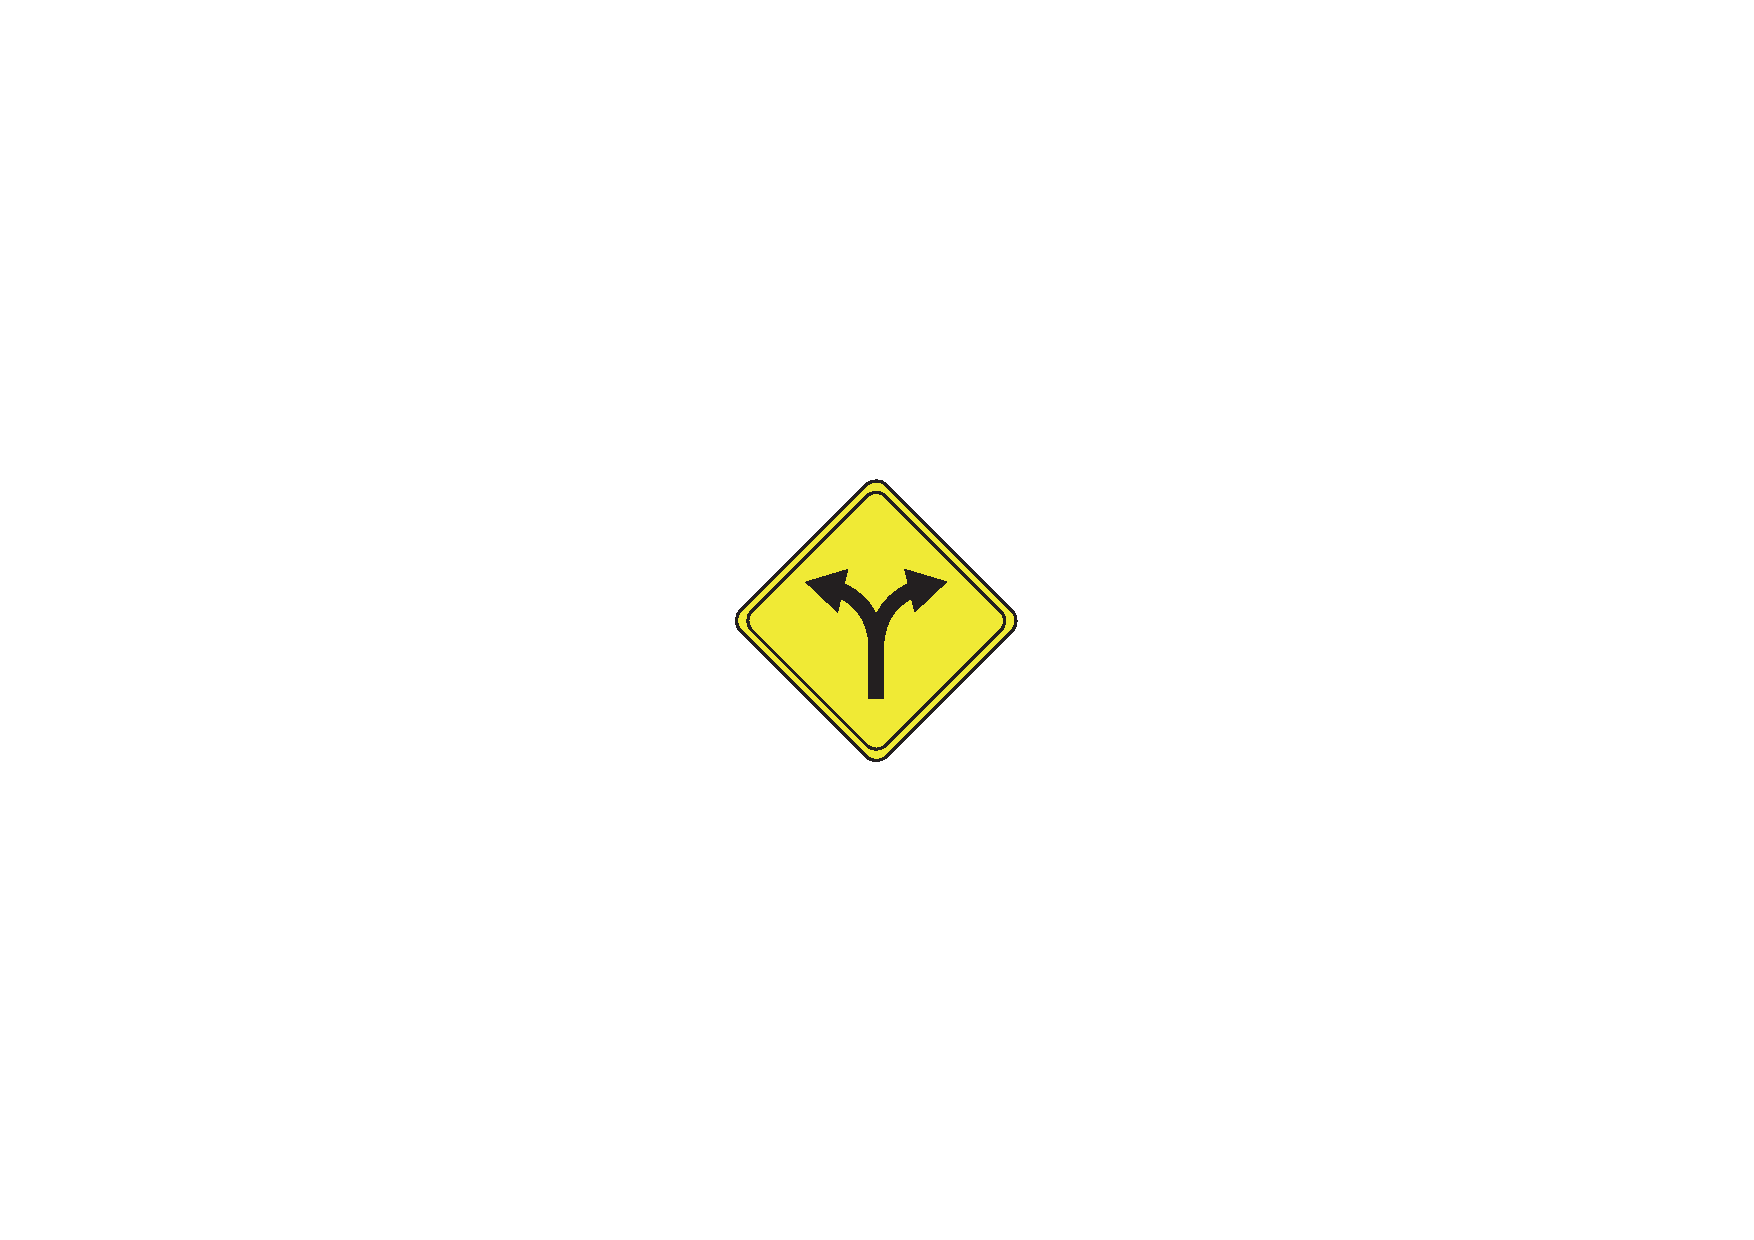
\includegraphics[width=1.5cm]{images/diversion} & \textbf{We digress\ldots} Boxes marked with this icon contain digressions and facts that are hopefully interesting but are probably tangential to the main flow of the exercise.\\
\end{tabular}

\FloatBarrier 
\section{The Raspberry Pi}

The most remarkable thing about the Pi is that, although it's a bit underpowered in many ways, it is capable of running the same full Linux Operating System as the machines that you'll be using in the labs for the duration of your studies, and which you'll undoubtedly encounter in your future careers. Actually we're going to be using slightly different flavours of Linux on the Pi and the lab machines, but the differences are fairly minor---more on that later. Let's get started. 

The Raspberry Pi itself is just the circuit board shown from the top in Figure \ref{figure:bare-rpi}. The case we've put yours in is clear plastic so you can see the Pi inside, but you're welcome to change it for another style if you prefer (there are plenty available to buy online, and lots of people have made their own unique ones just for the fun of it). The Pi is reasonably robust, and you can use it without a case, but obviously it's a bit more vulnerable if its not in a box of some sort. Figure \ref{figure:bare-rpi-underside} shows the Pi's circuit board from beneath, with an SD card inserted.

\begin{rpi}{Why Pi?}
  The Raspberry Pi apparently got its name because (a) lots of other computer systems have been named after fruit (you'll know of Apple and Blackberry, but in the past there has also been at least Apricot and Tangerine), and (b) the \wikipedia{Python_(programming_language)}{Python language} was one of the first things ported to run on it. The logo was created by Paul Beech, and is based on Buckminsterfullerene, a spherical fullerene molecule more commonly called a Buckyball. Its designer pointed out that a full buckyball has 32 faces, but that only 11 are visible in the 2D logo; and that the Raspberry Pi has a 32-bit processor and an ARM11 on board.

The ARM processor, on which the Pi and the vast majority of the world's other mobile devices are based, was originally designed by a team led by \wikipedia{Steve_Furber}{Steve Furber}, who is a Professor in this School.  
\end{rpi}

\begin{figure}
\centerline{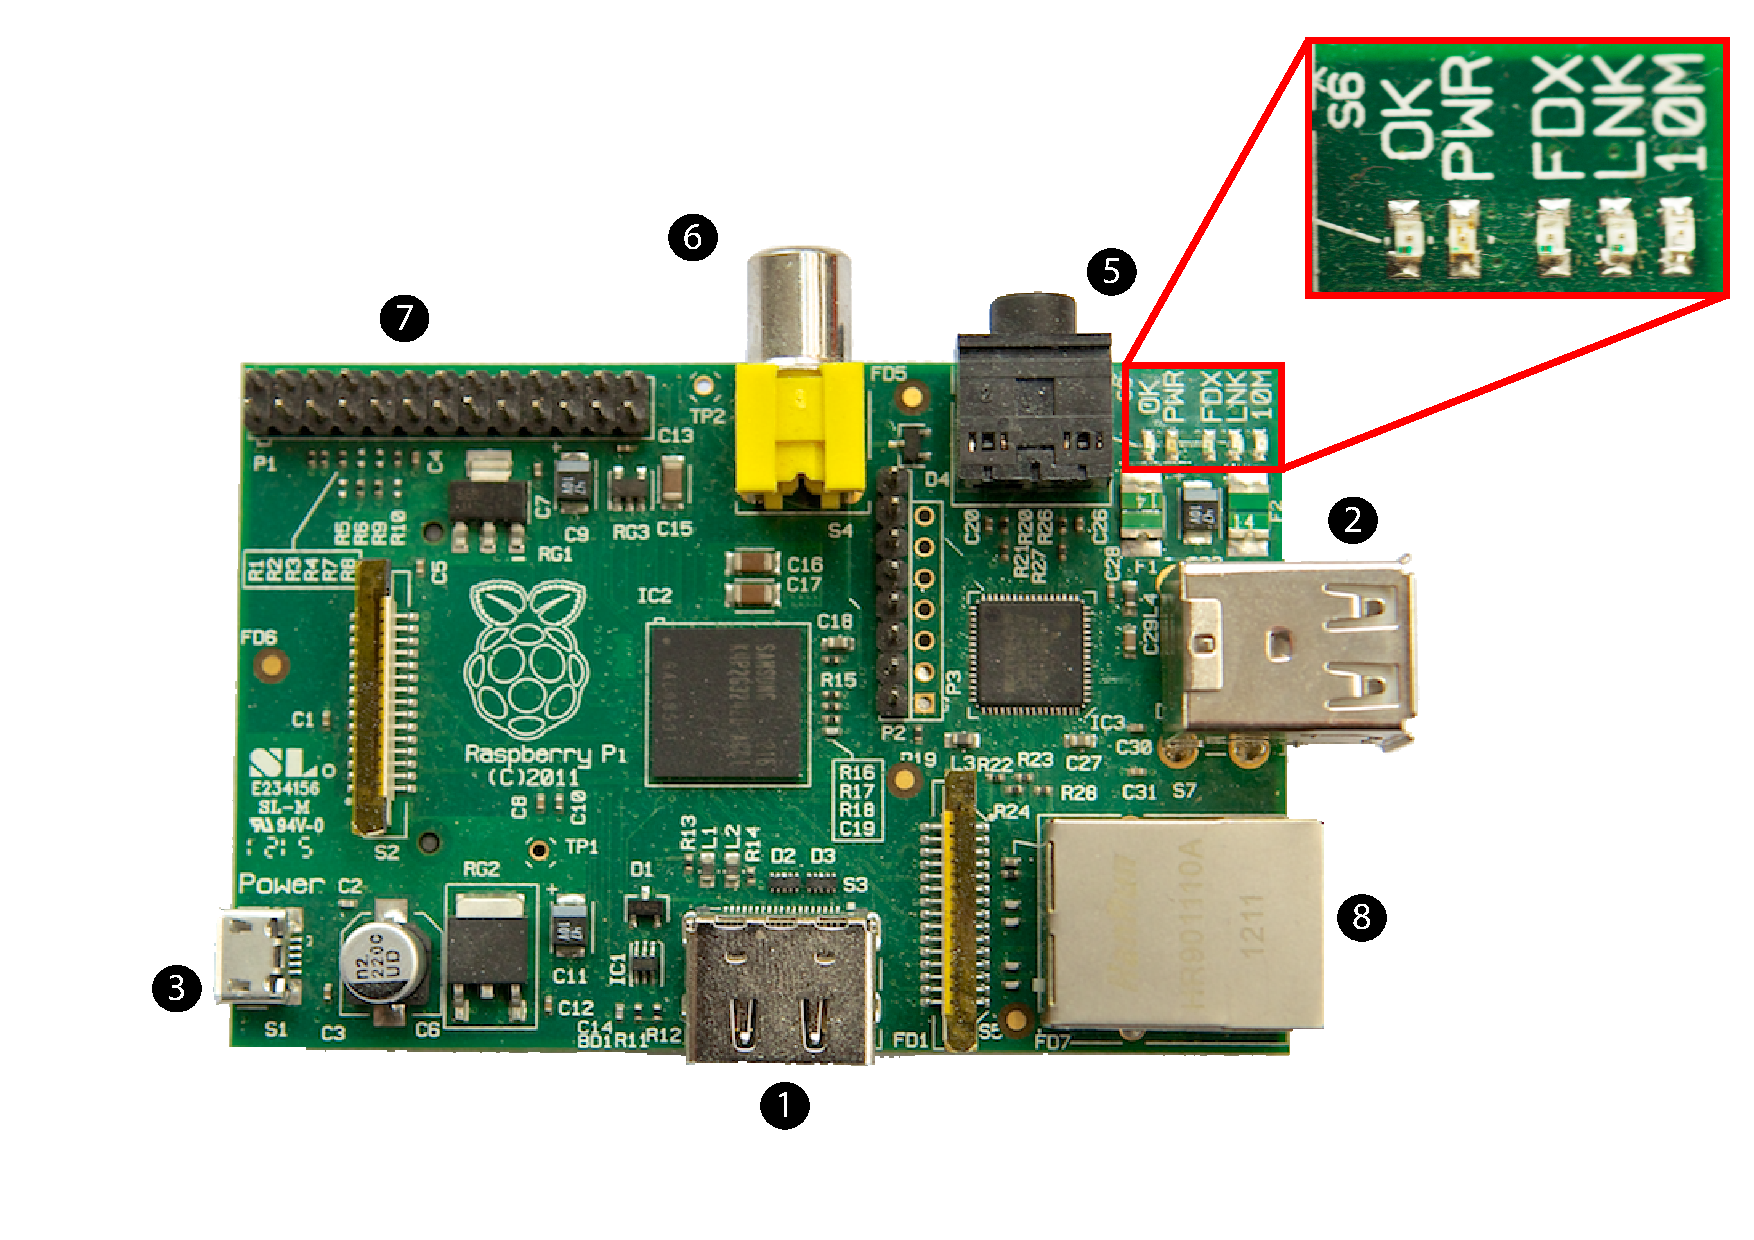
\includegraphics[width=15cm]{images/bare-rpi-annotated}}
\caption{An uncased Raspberry Pi, and an expanded view of the indicator LEDs at the board's top right. The numbered connectors are \protect\circled{1} HDMI output,  \protect\circled{2} USB,  \protect\circled{3} power,  \protect\circled{5} audio output,  \protect\circled{6} composite video out,  \protect\circled{7} General Purpose Input/Output (GPIO),  \protect\circled{8} Ethernet.}\label{figure:bare-rpi}
\end{figure}

\begin{figure}
\centerline{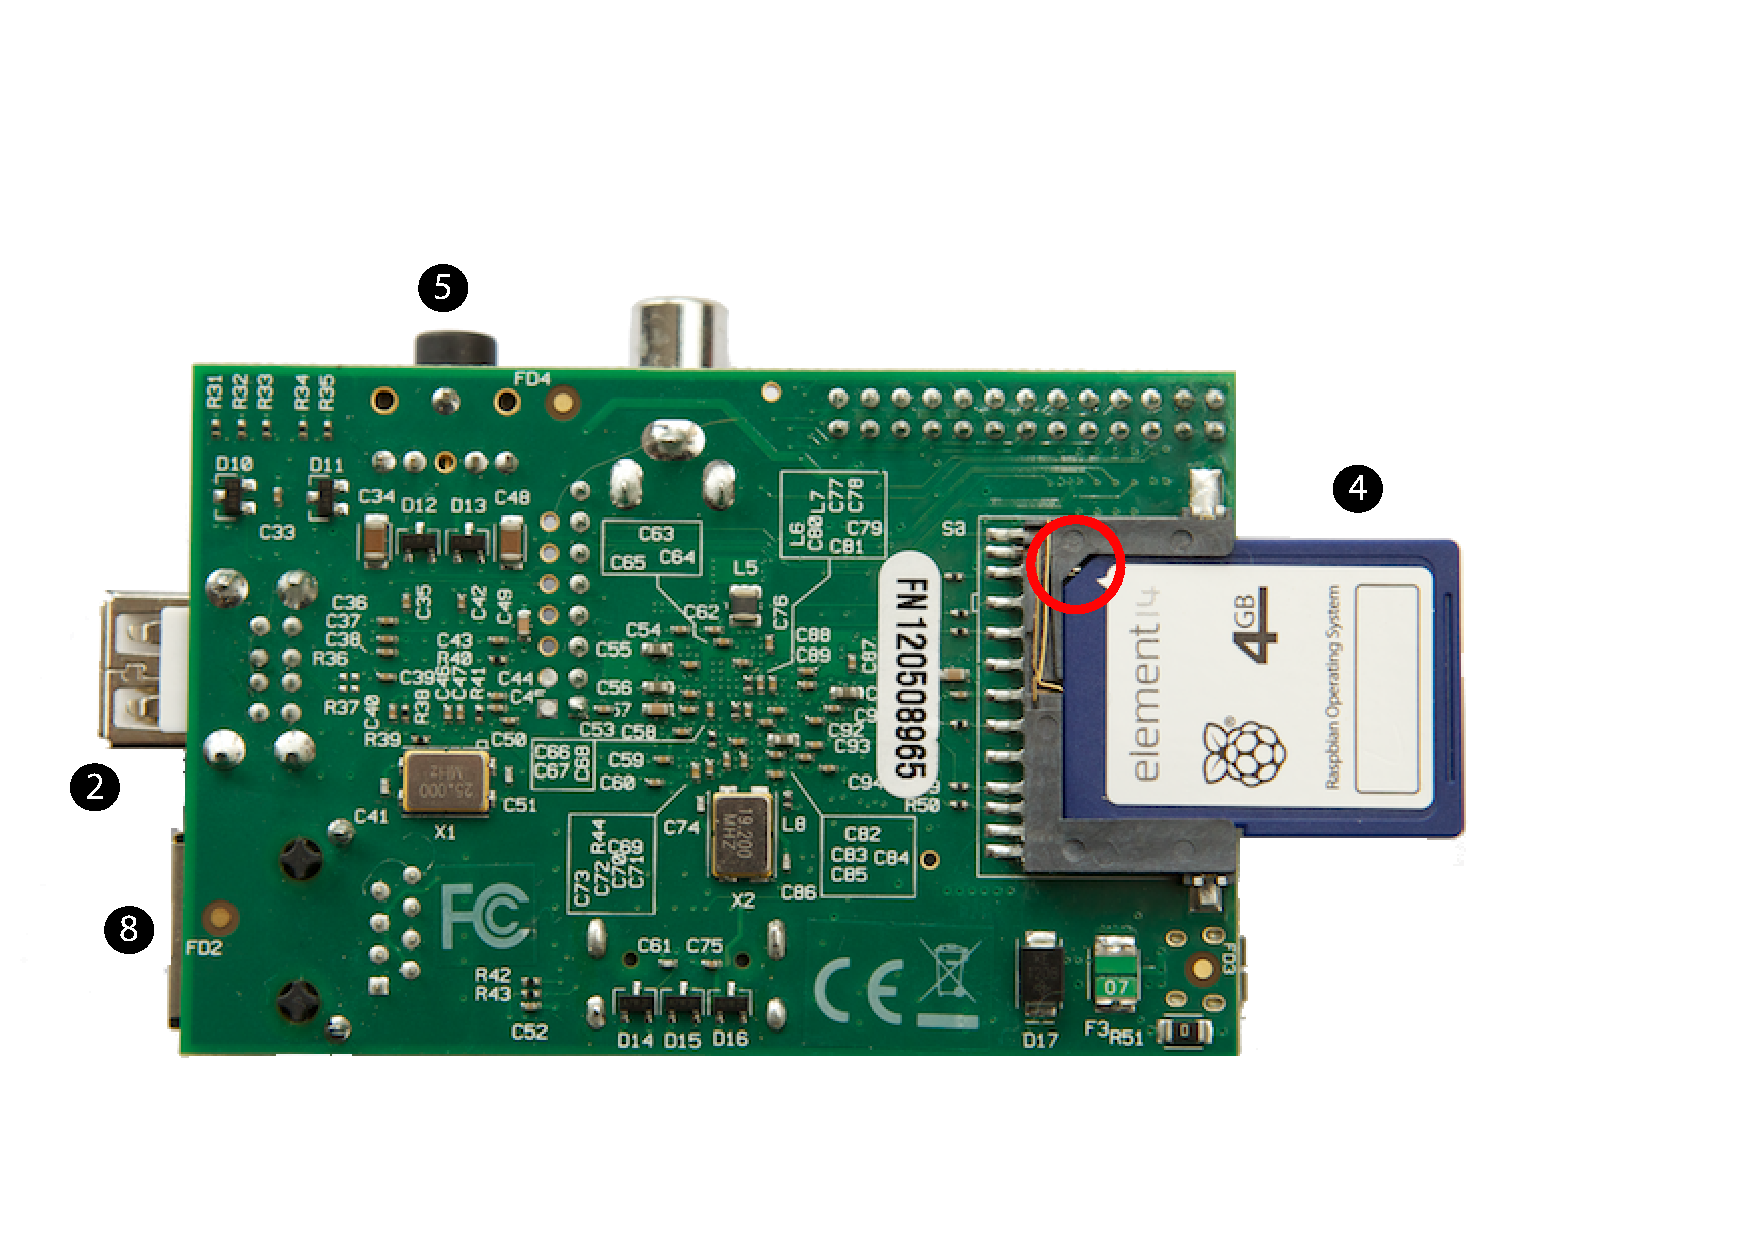
\includegraphics[width=15cm]{images/bare-rpi-underside-annotated}}
\caption{A naked Raspberry Pi. The circle indicates the location of the bevelled corner to orient the card. The ports are numbered as in Figure~\ref{figure:bare-rpi}, and in addition \protect\circled{4} shows the location of the SD (Secure Digital) memory card. The red circle indicates the locating bevel on the card.}\label{figure:bare-rpi-underside}
\end{figure}

It's important that you connect the Pi up in exactly the order specified here---so even if you are familiar with using a Pi, please don't jump ahead and plug everything in at once (no harm will come to the Pi if you do, but this exercise relies on your following our instructions closely). The monitors in the LF31 Lab are all fitted with an extra video lead for connecting up the Pis. Locate the HDMI lead, and plug this into the socket marked \circled{1} on Figure~\ref{figure:bare-rpi}. Next we'll need to connect a keyboard. Follow the cable that comes out the back of the keyboard towards where it vanishes into the desk, and you'll see an inline USB connector that will allow you to unplug the keyboard from the desktop PC and into one of the two USB sockets on your Pi; these are marked with \circled{2} on the Figure. It doesn't matter which USB socket you choose, but please make sure to reconnect this to the PC when you're done with these experiments, just as a courtesy to the next user. 

Next, we need to insert the \wikipedia{Secure_Digital}{Secure Digital} (SD) card that contains the Pi's operating system, and on which you'll be storing your own files. Look at Figure ~\ref{figure:bare-rpi-underside}, make sure the SD card is orientated correctly (note the position of the little cut corner) and gently push it into the socket; around half of the card will remain protruding outside the case. \textbf{Don't} plug a mouse in at this stage; you won't need it until the very last part of the exercise.

\begin{rpi}{Raspbian}
  The SD card we've provided for you has already had the standard Raspbian version of Linux written onto it (it's a version of the Debian release of Linux, tuned for the Pi). If you do manage to corrupt the operating system, or just want to start from scratch, then re-writing the SD card with a fresh image is reasonably straightforward: there are plenty of instructions online on how to do this, and we've provided you with a USB multi-card reader/writer that you can use for the job. The process does require access to what's called the `raw' device though, and on Linux that requires administrator access to the machine, so you'll have to use your home machine or someone else's Raspberry Pi to do this.

  Instructions on how to get hold of the files you'll need, and how to write them to the SD card on various operating systems are available at \url{http://www.raspberrypi.org/downloads}. You might want to think about getting a larger SD card in any case; the one we've given you is fine for the labwork we've set, but probably a bit on the small side for anything else. SD cards are widely available in shops and online, and aren't expensive. But you should check whether the specific card you're going to buy is compatible with the Pi before parting with any money---differences in the read/write speeds of some cards mean they don't play nicely with the Pi.
\end{rpi}

Now you're ready to power up the Pi. From the back of the monitor you'll notice a Micro USB cable (the same connector that you'll find on many modern smartphones and tablet devices). This goes into the socket marked \circled{3} on Figure \ref{figure:bare-rpi}. There is no power switch on the Pi, so as soon as the power cable goes in, it will start to boot (this strange term is explained in breakout box~\ref{boot box}): the red PWR LED should light up and stay on, and you'll also notice that the OK LED (which indicates SD-card activity) to its left also flickers. If any of the other three LEDs marked FDX, LNK, or 10M are lit, then that means you've already plugged a network cable into your Pi, in which case please unplug that now!

\begin{danger}{Pi Power} 
Like most other computers, the Pi doesn't like having its power removed without being shut down properly. Although you might get away with it, there's a reasonable chance of messing up the operating system if you remove the power while the Pi is in the middle of doing something. And because the Pi runs a multi-tasking operating system, it's almost always `doing something', so pulling the power out unexpectedly is always a bad idea. You're unlikely to damage the Pi's hardware like this, but you may find that you lose work, and may have to reinstall the operating system. For instructions on how to shut the Pi down safely, see Section \ref{section:shutdown}.
\end{danger}

Refer to Figure~\ref{figure:monitorswitch} and switch the Input Selection on the monitor from VGA (which is the input used by the PC under the desk) to DVI (the cable you've connected your Pi to is a HDMI to DVI cable), and all being well you should see a black screen containing the Raspberry Pi logo at the top left, and white text that scrolls up the screen as the Pi boots. When the boot process finishes for the first time (it will take somewhere about 20--30 seconds), if all has gone well you should see the Pi's configuration tool appear (see Figure \ref{figure:raspi-config}).

% TODO: needs a photo of the monitor / switch here
\begin{figure}
\centerline{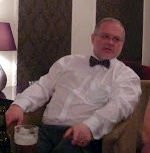
\includegraphics[width=5cm]{images/mysteryimage}}
\caption{The Input Selection switch on the monitor.}\label{figure:monitorswitch}
\end{figure}

\begin{diversion}{Booting}
\label{bootbox}
The phrase `booting' to refer to the process of starting up some computer system has become quite commonplace, but its origins are rather strange. It's thought to have first been used in early 19th Century America as a way of describing an obviously impossible action such as to ``pull onself over a fence by one's bootstraps''. These days it is used to refer to any self-sustaining process that is able to happen without external help. 

So why is starting a computer a bootstrapping process? In order for you as a user to be able to run a program, the computer needs an operating system. But in order to load its operating system, it needs some instructions that tell it how to understand the file system. And in order to load the instructions that tell it how to understand the file system it needs to\ldots well, you get the idea. In reality, most computers have a very small set of instructions hardwired into them that begin the process of loading a  slightly more complex `bootloader', which then begins the process of loading the OS kernel and any modules needed to interact with the hardware, and then starts loading services and features of increasing sophistication that rely on the simpler ones loaded previously to function. 

As an aside, you want to consider this: if you need a text editor to write programs, how did the first text editor (which is itself a program) get written?
\end{diversion}

\begin{figure}
\centerline{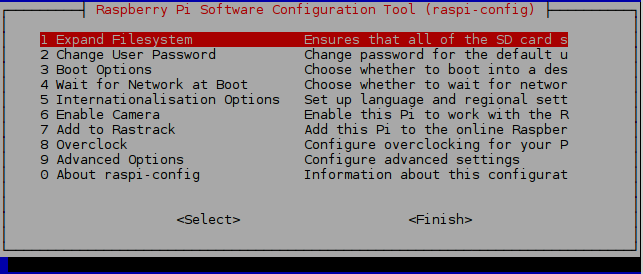
\includegraphics[width=13cm]{images/raspi-config.png}}
\caption{The Raspberry Pi config tool. The highlight bar can be moved between the different controls using the Tab key, or up and down in the menu using cursor keys.}\label{figure:raspi-config}
\end{figure}

Before using the Pi for real, you'll need to perform one task using this menu. Use the up and down cursor keys to move the selection bar to the \ttout{expand\_rootfs} option, and press Enter. You'll see a confirmation that `Root partition has been resized. The filesystem will be enlarged upon the next reboot'. If that doesn't mean anything much to you right now, don't worry, we'll come back to an explanation of that later (see Section~\ref{section:expandfs}). For now just press Enter again to get back to the main menu. 

At this stage you could tweak various other options that affect the display and the layout of keyboard being used; but conveniently the defaults set on the Pi will do just fine for now (it is a mostly British invention after all, so it defaults to UK keyboard layout!) Use the Tab key to move the red highlight to \ttout{<Finish>}, and hit Enter again. The Pi will reboot (an example of what this looks like is shown in Figure \ref{figure:piboot}) and this time when the process finishes you'll be presented by a UNIX login prompt which will say something like:

\begin{figure}
\centerline{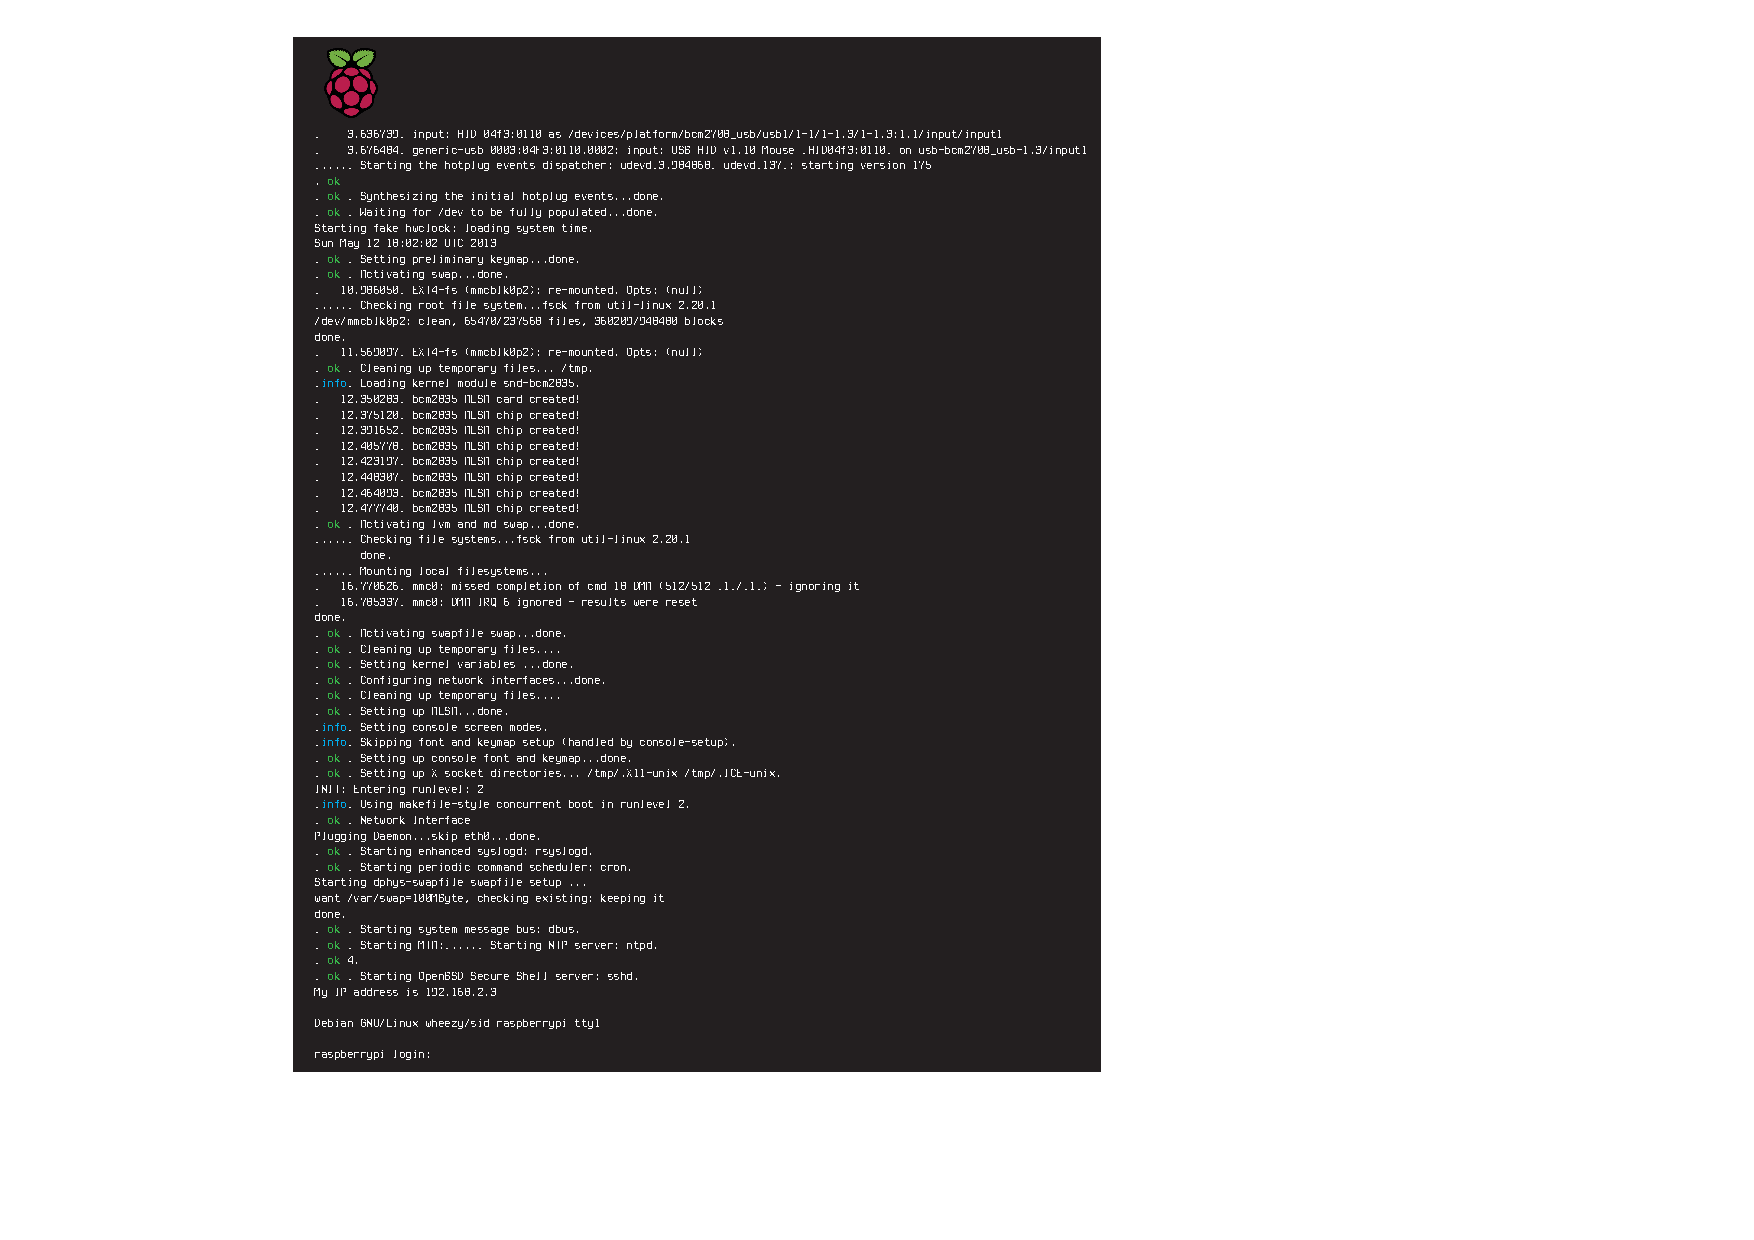
\includegraphics[width=15cm]{images/bootscreen}}
\caption{A sample Raspberry Pi bootscreen. The exact layout and details may vary depending on the size/shape of the screen and the configuration of the Pi.}\label{figure:piboot}
\end{figure}

\begin{ttoutenv}
Debian GNU/Linux wheezy/sid raspberrypi tty1

raspberrypi login:
\end{ttoutenv}

At the login line enter \totype{pi} as the username, and when prompted for the password, type \totype{raspberry}. \textbf{Note that the username will appear on screen as you type it, but the password will not} (so make sure you're typing carefully!) You should see:

\lstset{moredelim=[is][\textbf]{|}{|}}
\begin{lstlisting}
Last login: Mon Feb 16 14:46:27 2015
Linux raspberrypi 3.18.7-v7+ #755 SMP PREEMPT Thu Feb 12 17:20:48 GMT 2015 armv7l

The programs included with the Debian GNU/Linux system are free software;
the exact distribution terms for each program are described in the
individual files in /usr/share/doc/*/copyright.

Debian GNU/Linux comes with ABSOLUTELY NO WARRANTY, to the extent
permitted by applicable law.
|pi@raspberrypi ~ $|
\end{lstlisting}


%

The last line of this text (which is shown in bold here but will be green and blue on your screen) is the command prompt. It might look innocent enough, but in the right hands, the command prompt is one of the most powerful ways of controlling a computer. It may feel a bit odd at first if you're used to a graphical interface, but being comfortable with issuing instructions to a machine via a textual command-line rather is a crucial skill that you'll need during your studies here at University, and also in your future career.

\begin{diversion}{Don't be a WIMP}
The familiar Windows, Icons, Menus and Pointer (WIMP) paradigm used on most graphical desktop environments is enormously powerful, but it's not suitable for every task, and understanding when you're better off using the command-line or a keyboard shortcut instead will make you a lot more efficient.

Sometimes the clumisness of the GUI comes from the fact that there's no convenient visual metaphor for a particular action; how do you graphically represent the concept of `rename all the files I created yesterday so they start with a capital letter'? 

But a lot of the time the issue is simply that it takes much longer to do some things with the mouse than it does with a keystroke or two. Every time you use the mouse, a little time is wasted shifting your hand off the keyboard and a little more time used up tracking the pointer between the on-screen widgets. For casual use, this wasted time really doesn't matter. But as a computer scientist you're going to be spending a lot of time time in front of a machine, and all the seconds wasted moving the mouse pointer around add up. 

What's really fascinating here, though, is that although the keyboard versus mouse debate is one that has been running for at least the mid-1980s, there isn't a clear winner, or even any definitive guidelines as to when one is better than the other. 

In any case, you should definitely learn the keyboard shortcuts for the most common operations in your favourite tools, and a handful of useful command-line tools. For example, when you're writing code you'll be saving files very regularly; maybe even several times a minute when you're debugging. There are two options for this: 1) move hand off keyboard to mouse; use pointer to find the `File' menu, from the file menu move the pointer to the `Save' option; move hand from mouse back to keyboard. Or 2) Press the combination of keys that perform the `save' function. Which do you think is faster?

And think carefully about the best tool for the job; sometimes it'll be the mouse/menu combination, but perhaps more often than you might think, a few selected commands may get the job done considerably more quickly. In particular, you've probably had more experience of doing things the GUI-way up until now, so if it's not obvious which is the better choice for a particular task, we suggest you go for the command-line option until you're familiar enough with the pros and cons of both approaches to make an informed decision each time.
\end{diversion}

The default command prompt on the Pi consists of four components shown in Figure \ref{figure:prompt}.

\begin{figure}
\centerline{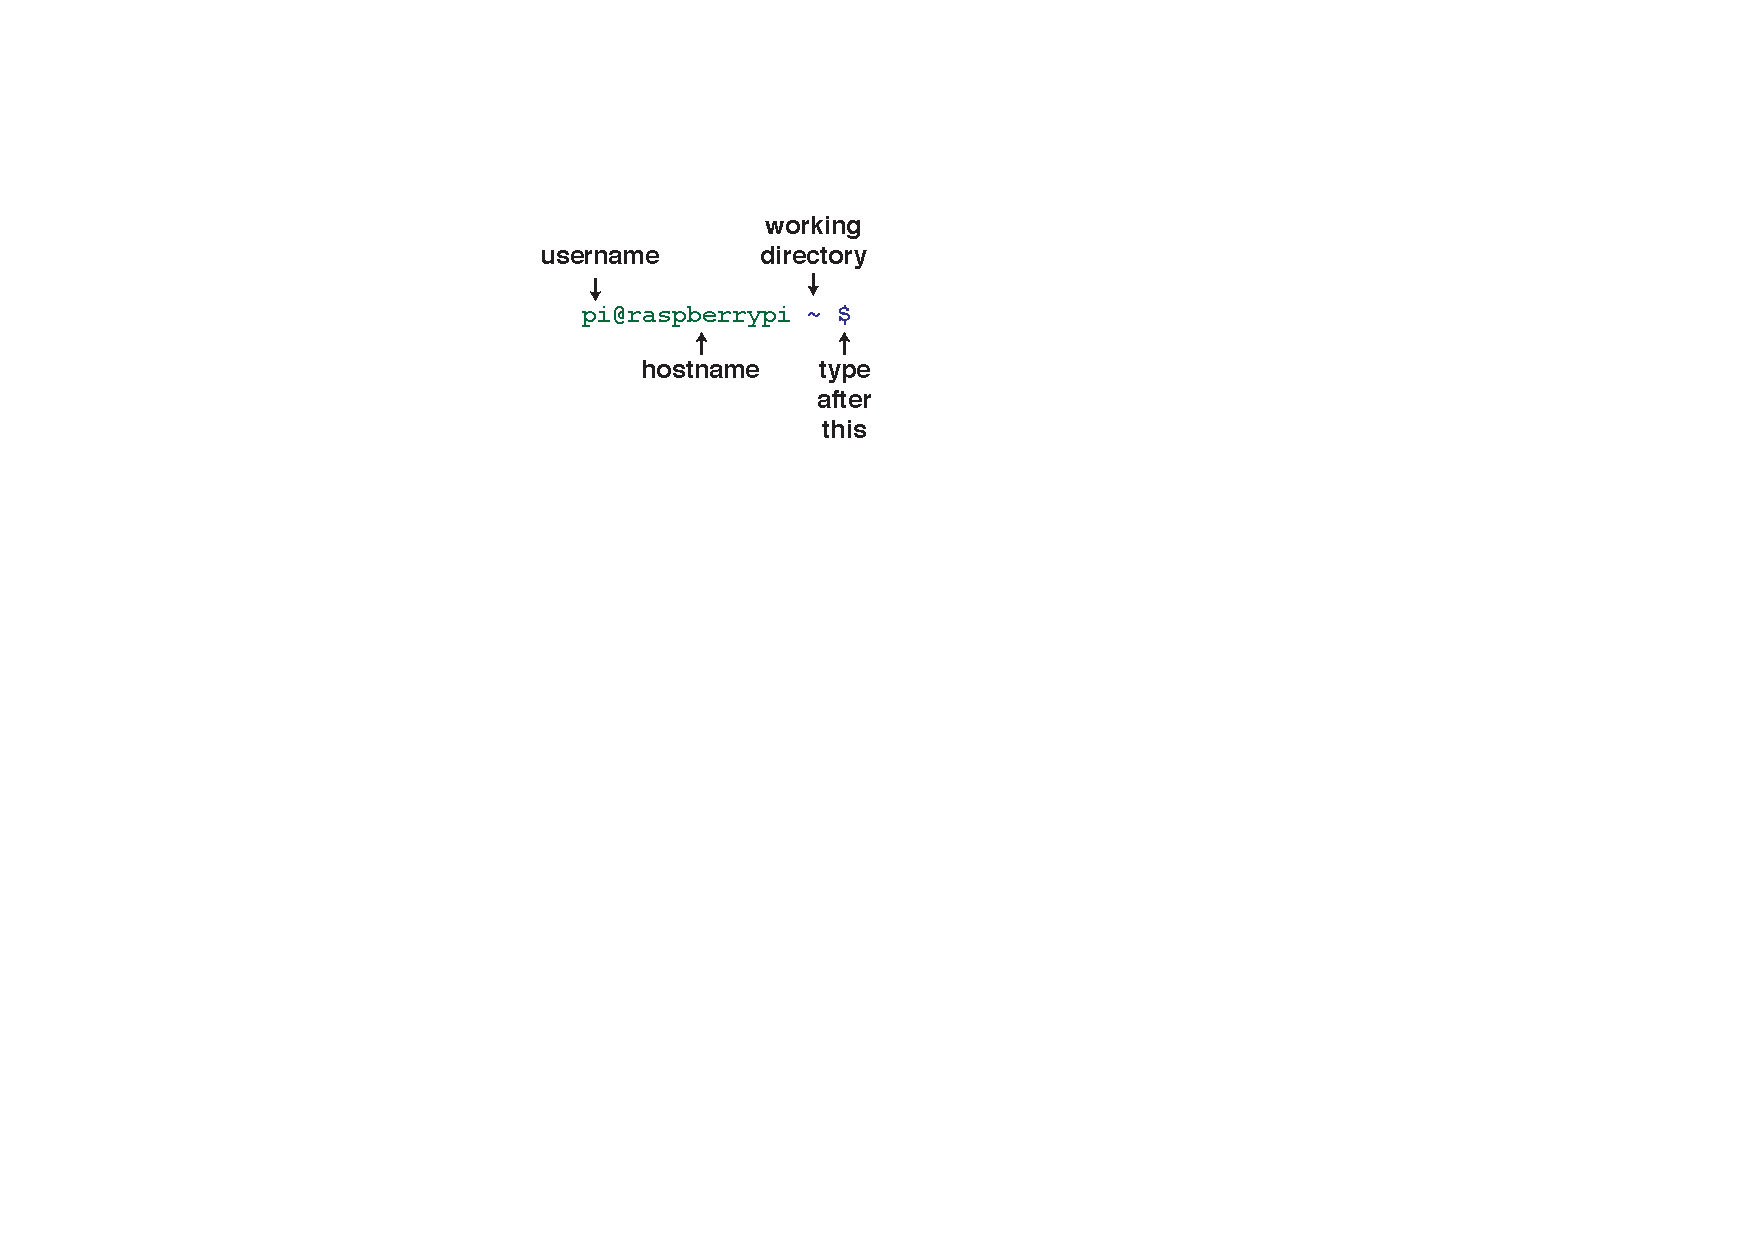
\includegraphics[width=7cm]{images/default-prompt}}
\caption{The different components of the Pi's default command prompt.}\label{figure:prompt}
\end{figure}


\begin{itemize}
\item To the left of the \ttout{@} symbol is the name of the user, and in this case that's \ttout{pi}, since you've just logged in under that name
\item To the right of the \ttout{@} is the hostname of the machine, which on a Raspberry Pi is quite reasonably set to \ttout{raspberrypi} by default.
\item The \texttildelow{} tells you where in the filestore you're currently working. We'll explain this in a lot more detail later on, for now all you need to know is that the \texttildelow{} symbol is called a \textit{tilde} (pronounced something like till-duh, though locally its often referred to colloquially just as a `twiddle'), and is used here to refer to the `home' of the current user. 
\item the \$ symbol signifies that you can type your commands from here on. 
\end{itemize}

You can change this prompt to something more or less verbose later, but for now we'll leave it as it is. For simplicity in these notes, we'll use the \$ notation from now on to mean `type something at the command prompt and press Enter'. So for example

\begin{ttoutenv}
$ echo Hello World
\end{ttoutenv}

\noindent means `type \totype{echo Hello World} at the command prompt and then press Enter' (you can do this if you like; the result will be that `Hello World' gets `echoed' back to you on the next line of the screen). 

Before we do any real work on the Pi, we should make it a bit more secure than it currently is. Remember, you've logged in using the default username `pi' and the default password `raspberry', so anybody else could do the same. To change the password to something that's unique. For inspiration and advice on creating good passwords, see Figure \ref{figure:xkcd-password}.

\begin{figure}
\centerline{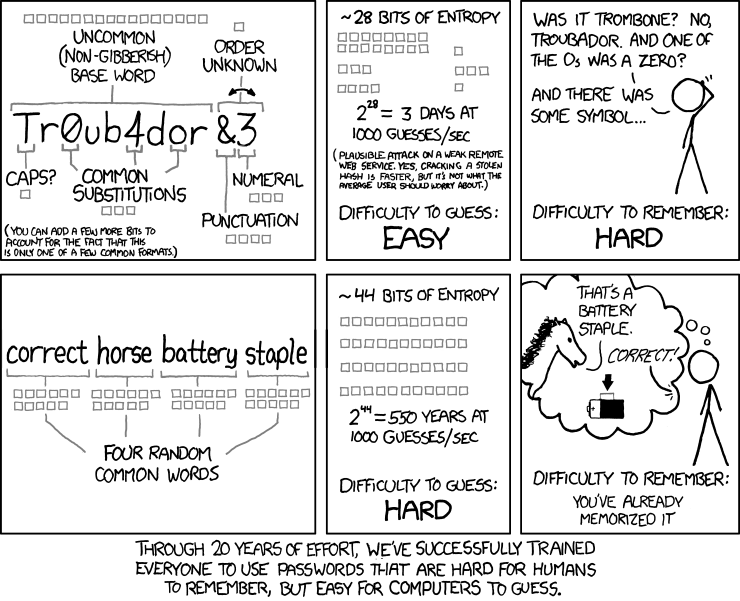
\includegraphics[width=13.5cm]{images/xkcd-password-strength}}
\caption{XKCD's take on password creation \url{http://xkcd.com/936/}}\label{figure:xkcd-password}
\end{figure}

The command to change the password is \totype{passwd}; typing this at the command prompt and entering your current (i.e. `raspberry') and new password (twice, to be sure), should look like this:

\begin{ttoutenv}
$ passwd
Changing password for pi.
(current) UNIX password:
Enter new UNIX password:
Retype new UNIX password:
\end{ttoutenv}

\noindent Note in the above, we're using lines that don't start with the dollar symbol to show output as a result of what you've typed, and that none of the passwords you're typing actually appear on screen for obvious sneaky over-the-shoulder-peeking reasons. \textbf{Don't forget this password: there's no easy way to get back into your Pi without resetting everything.}

\begin{danger}{Memory Loss} 
Although the Pi uses a fairly standard UNIX operating system, it's probably not quite as secure as a normal desktop machine because of its small size and easily-removable storage media. Once the Pi has booted from the SD card, it's about as secure as any other Linux machine. But because the memory card is easily removable, it can trivially be connected to another machine as a `removable media' device; and at that point the host machine can almost certainly see its contents, including any of the files you've created, because the filesystem itself isn't encrypted. And because the Pi is small and portable, it's easier to lose it than a laptop or desktop machine; so, be careful!
\end{danger}

Now that your password isn't the same as the `out of the box' Pi one, it's safe to plug your Pi into the network. There's a spare ethernet cable poking out of the desk; plug that into the appropriate socket on your Pi (number \circled{8} on Figure~\ref{figure:bare-rpi}) and you should see the FDX, LNK and 10M LEDs light up. To confirm that you're now connected to the network, use the \totype{ping} command, which sends a low-level network message to a designated place and checks for a response, to see if you can reach our School's web server. 

\begin{ttoutenv} 
$ ping www.cs.manchester.ac.uk
PING waldorf.cs.manchester.ac.uk (130.88.194.191): 56 data bytes
64 bytes from 130.88.194.191: icmp_seq=0 ttl=52 time=37.914 ms
64 bytes from 130.88.194.191: icmp_seq=1 ttl=52 time=40.392 ms
64 bytes from 130.88.194.191: icmp_seq=2 ttl=52 time=41.006 ms
\end{ttoutenv}

Each of the lines starting with `\ttout{64 bytes}' represents a short response from the machine you've just pinged, and you're shown the round-trip time for ping's data to leave your Pi, find (in this case) \fname{www.cs.manchester.ac.uk} on the network, and return back to your Pi. Since we're just using ping here to give us some confidence that the network is okay, we don't need to leave it pinging away for ages, so let's stop the ping command in its tracks. Hold down the control key (marked `ctrl' on the keyboard), and press `c'. This will signal the currently executing command that it should stop what its doing and return to the command prompt (quite often this is referred to as ``control-c'ing'' a command, and it will have the same effect on the majority of command-line tools).

\begin{diversion}{Ping}
  The \totype{ping} command is named after its use in the field of active sonar, where an actual `ping' sound was sent through water, and distance calculated by listening for the echo to return. It's the classic boingy pingy noise associated with submarine movies! 
\end{diversion}

\section{The Unix Shell}

Before doing anything else, let's take a step back and look in a bit more detail at what you've just done. You have been
interacting with a \wikipedia{Shell_(computing)}{shell}: a program that prompts
the user for commands, accepts them, executes them and displays the
results. A shell is just a program running on the Linux operating system like any other program---it's not `built in' to the operating system in any special way, it just happens that by default, the Pi is set up so that when a user logs in, the first program that gets executed on behalf of that user is an interactive shell that allows the user to execute further programs themselves. Later in this course we'll look at the file that determines which program gets executed first for a user, and indeed at the order in which programs are run by the operating system as it boots up, because in Linux all of these things can be easily configured by changing a few lines in the appropriate text file. But for now, it's enough to understand that the shell is just a program that interacts with the user via the keyboard and display, and allows you to execute commands to do useful things.

\begin{diversion}
Unix has many shells: the first shell was called the `Thompson' shell (also known as just `sh', and pronounced ``shell''), written by Ken Thompson for the first Unix system; then came the `Bourne' shell (also called `sh'), written for a later commercial version of Unix by Stephen Bourne. You have just been using the Free Software Foundation's `Bourne Again' shell (another pun-name taking a dig at its commercial fore-runner), or `bash'. The various different shells offer the user different facilities: `sh' is rather
primitive compared to the more modern ones. However, their basic
functionality is always the same: they accept commands from the
\textbf{standard input} (for now, we can treat that as meaning `the keyboard'), execute them, and display
the results on the \textbf{standard output} (i.e. for now `the screen', which in
this case was the entire screen, or \textbf{console}). Shells repeat
this process until they have reached the end of their input, and then
they die. Unix shells are rather like \textbf{Command Prompt} windows in Microsoft
Windows, except that Unix shells are considerably more sophisticated.
\end{diversion}

\section{The Unix File System}

Next we're going to explore the Pi's filesystem a little. You'll be familiar with the idea of a hierarchy of files and folders from whatever graphical environment you're used to using on desktop or mobile devices: files represents things that you've created or downloaded such as documents, images or movies, and folders are a way of organising these into related collections. By putting folders inside folders, you can organise your stuff starting with general concepts such as `Photographs' and ending up with much more specific collections, e.g. `Holidays', then `Bognor Regis 2013'. 

Interacting with a standard UNIX filesystem via the command-line uses similar concepts (actually, it's the graphical environment that's being `similar' here really, since the UNIX command-line existed quite some time before anything graphical appeared). Files are called files, but what are commonly represented as `folders' in graphical environments are more correctly called `directories' when we are operating at this level (and we'll call them directories from now on, because it'll make many of the command names make more sense). 

Let's first see what stuff we already have on our Pi. The \totype{ls} command lists files and directories. Type it now, and you should see that two folders have already been created for you, one called \fname{python\_games} and the other called \fname{Desktop}. 

\begin{ttoutenv}
$ ls
Desktop python_games
\end{ttoutenv}

When we're using a command-line prompt, we have the notion of of \wikipedia{http://en.wikipedia.org/wiki/Working_directory}{current working directory} which is the directory that we're currently `in'. Any commands we issue that don't specify another directory are assumed to refer to the current working directory; so \totype{ls} on its own really meant `run the list command on my current working directory'. 

Let's say we want to look at the contents of the \fname{python\_games} directory. There are several ways of doing this, but for now we'll break the process down into simple steps. Use the \totype{cd} command to Change Directory to \fname{python\_games}:

\begin{ttoutenv}
$ cd python_games
\end{ttoutenv}

\noindent and then use the \totype{ls} command to list its contents. You should see a long list of files: some are programs written in the Python programming language (these files end in .py), others are images or sounds used by those programs (ending in .png or .wav). At the prompt type:

\begin{ttoutenv}
$ python wormy.py
\end{ttoutenv}

to start a simple version of the classic `Snake' game. You can guide your green snake around the screen with the cursor keys; you score a point every time you eat one of the red squares, and extra segment gets added to your snake. The game finishes if you crash into the edge of the screen or eat yourself. Once you've convinced yourself this is working (don't spend too long playing the game!), press the Escape key to return to the command prompt. You'll be writing a more sophisticated version of this game soon enough in the Java labs.

Take a look now at the command prompt; whereas before it was just
\\
\\
\totype{pi@raspberrypi \texttildelow{} \$}
\\
\\
it has now become
\\
\\
\totype{pi@raspberrypi \texttildelow{}/python\_games \$}
\\
\\
to indicate that we've changed our current directory to \fname{python\_games} (remember the \texttildelow{} symbol means `home directory', so \fname{\texttildelow{}/python\_games} really means 'a subdirectory called python\_games which is in my home directory').

%\FloatBarrier
\section{The UNIX filesystem}

In UNIX, as with most other operating systems, the files and directories you create can have more-or-less any name you like. It is very sensible to give them names which mean something and make their purpose clear. This is despite some of the traditional file names in Unix being rather cryptic---this is particularly true for most UNIX commands. You'll get used to that. 

\begin{danger}{File name formats}
The filesystem on your Pi (which uses a type of filesystem called `ext4') \textit{case sensitive}, which means that \fname{Hello.txt} and \fname{hello.txt} are treated as different files because they have different case letters in their names. The filesystem used by Microsoft Windows since XP (called `NTFS') is also case-sensitive. Apple's OS X, however uses `HFS Plus' (which usually appears as `Mac OS Extended (Journaled)'), and this is not a proper case-sensitive file system; although it will remember whether you called a file \fname{Hello.txt} or \fname{hello.txt} so files \textit{appear} to be case sensitive, the OS itself treats them as being \textit{the same file}! The same is true for the FAT32 filesystem used on most removable USB drives -- because it's one of the few formats that's understood by Windows, Mac and Linux. 

Most of the time this isn't a problem, but you should be careful of the effects when copying files from one filesystem to another, especially if you are using a USB drive to transfer files from a Linux box to somewhere else. For example, if you have two files in the same directory on Linux but with different capitalisation, one file will overwrite the other when you copy them onto your USB drive (and which one survives will depend on the order in which they are copied). One way around this problem is to use something like \totype{tar} or \totype{zip} to bundle the files up into a single archive file, and then transfer that via the USB drive. 
\end{danger}

\begin{linux}{Spaced out filenames}
Because of its roots in the early days of computing long before the advent of graphical user interfaces, UNIX filenames tend not to have spaces in them because this conflicts with the use of a space to separate out commands and their parameters. The UNIX filesystem does allow spaces in filenames, but you'll have to use a technique called `escaping' if you want to manipulate them from the command line; this involves prefixing spaces in filenames with the backslash character \textbackslash{} to tell the command line not to interpret what follows the space as a new parameter. For example, a file called \fname{my diary.txt} would be typed as \fname{my\textbackslash{} diary.txt}. It's a bit ugly, but it works fine. 
\end{linux} 

As you already know, directories are created within directories to create a hierarchical structure. But where is the `top' directory? Surely that has to go somewhere? On each machine, there is one directory called `/' which is referred to as the \textit{root}, which is not contained in any other directory. All other files and directories are contained in root, either directly or indirectly. The root directory is written just as \fname{/} (note this is the opposite slanting slash character to that used in Windows, which means something similar but different). 

If we wish to talk about the file \fname{y} within the directory, \fname{x} we write \fname{x/y}. Of course, \fname{y} may itself be a directory, and may contain the file \fname{z}, which we can describe as \fname{x/y/z}.

You can think of this structure as defining a tree, with \fname{/} as the root (hence its name), directories as branches, and other files as leaves. You will study trees as abstract data structures, later in this year, and in Year 2, but this simplified model of the Unix file system structure will do for now. 

One really important, and slightly strange thing to get used to, though, is that computer science trees grow upside down, so although we call them trees, the `root' is usually thought of as being at the top, and the `leaves' at the bottom. You'll hear phrases like `go up to the root directory, and then down one level to the home directory'. We normally think of the root directory as being at the top of the tree. (For those of you who are interested: Unix actually allows links, which means the structure can really be a cyclic graph. Links are similar to, but fundamentally not the same thing as, shortcuts in Windows.)

Apart from \fname{/} there are two more directories of special note:
\begin{itemize}
\item Your \textit{home directory} is the directory where you find yourself when you log in. It might be tempting to think of this as being the `top' of the tree (and for every-day purposes thinking this way is probably okay), but in reality your home directory is probably one or more levels away from the root of the file system. We'll find out where this is on the Pi shortly. 
\item Your \textit{current working directory} is the one you are working in at a particular moment. \end{itemize}

So let's see where we are in the Pi's filesystem at the moment. Assuming you're following these instructions properly you should still be in the \fname{python\_games} directory (check the command prompt to confirm this is the case). To go back to our home directory, we can use the \totype{cd} command without any parameters:
\begin{ttoutenv}
$ cd
\end{ttoutenv}

You should see the command prompt change back to being as it was when we first logged in. So where in the filesystem is our home directory? We can find out where we currently are using the \totype{pwd} command, which stands for Print Working Directory:

\begin{ttoutenv}
$ pwd
/home/pi
\end{ttoutenv}

So apparently we're in a directory called \fname{/home/pi} which sounds plausible enough. Notice that the \totype{pwd} command has returned us an \textit{absolute pathname}, because \fname{/home/pi} starts with a \fname{/} character, so we now know that the home directory for the user \fname{pi} is in a directory called \fname{home} which itself is a subdirectory of root. 

Let's confirm that this is true. Issue the command:
\begin{ttoutenv}
$ cd /
\end{ttoutenv}

which just means `change directory to the root directory' and use the \totype{ls} command to look at the root directory's contents. You'll see several directories with names like \fname{bin}, \fname{boot}, \fname{dev} and \fname{lib}. Most of these contain `housekeeping' files for the operating system, and at this stage you don't need to know what's in them (though Table \ref{table-dirs} gives you a brief description if you're interested). The one called \fname{bin} is quite interesting though, so let's investigate that by typing: 

\begin{ttoutenv}
$ cd bin
$ ls
\end{ttoutenv}

\noindent You should see a fairly long list of files. Look carefully, and you'll find two names that you recognise: \totype{ls} and \totype{pwd}. These are the `binary executable' files for the commands that you've just been using (which is why they are in the `bin' directory, which is short for binary). In UNIX, most commands are not `built into the system', but are just programs put in a special place in the filesystem that are picked up by the command-line when you type things. This makes UNIX very easy to extend with new features; you just write a program to do what you want, and put it in the right place. We'll look at how the system knows where to find commands later, and explore several of the other commands you can see in this directory as well. 

We now need to get back to our home directory. You should by now be able to think of at least four different ways of getting there!

\begin{enumerate}
\item \totype{cd} on its own means `take me directly to my home directory'.
\item We know that the tilde symbol also means `my home directory', so \totype{cd \texttildelow{}} will also work (though at the expense of two extra keystrokes!)
\item We could go back to the root directory by first typing \totype{cd /}, then \totype{cd home} and finally \totype{cd pi}, or 
\item We could go straight from where we are now (which in \fname{/bin}, remember) by typing \totype{cd /home/pi}. 
\end{enumerate}

Now we're back in our home directory (check the command prompt to make sure), you may have noticed that our commands for navigating around the filesystem are missing one feature. We can go to the `top' of our home directory easily enough; and we can go straight to very top of the whole filestore using \totype{cd /}; and we know how to descend into a subdirectory (e.g. \totype{cd python\_games}). But how do we go up one level? If we were in some nested subdirectory several levels below our home, and wanted to go just one level back up the tree, it would be very tedious to have to start back at our home directory and traverse back down to where we wanted to be. 

UNIX represents the idea of going `up' one directory with the \fname{..} symbol (that's two fullstops typed immediately after one another with no spaces). So if you are in, say, \fname{python\_games} and want to go \textit{back up} to the directory above, you could type:

\begin{ttoutenv}
$ cd ..
\end{ttoutenv}

You can mix in the \fname{..} notation in relative and absolute paths anywhere you like. So, assuming you are still in \fname{python\_games}, how could you get into \fname{/bin} using only a \textit{relative} path in the \totype{cd} command? Yes, this is a slightly artificial exercise because the simplest solution would just be to use the absolute path \totype{cd /bin}, but just go with the flow for now and work it out using a relative path. The answer is shown in Figure \ref{figure:simple-navigation}. 

\begin{figure}[t]
\centerline{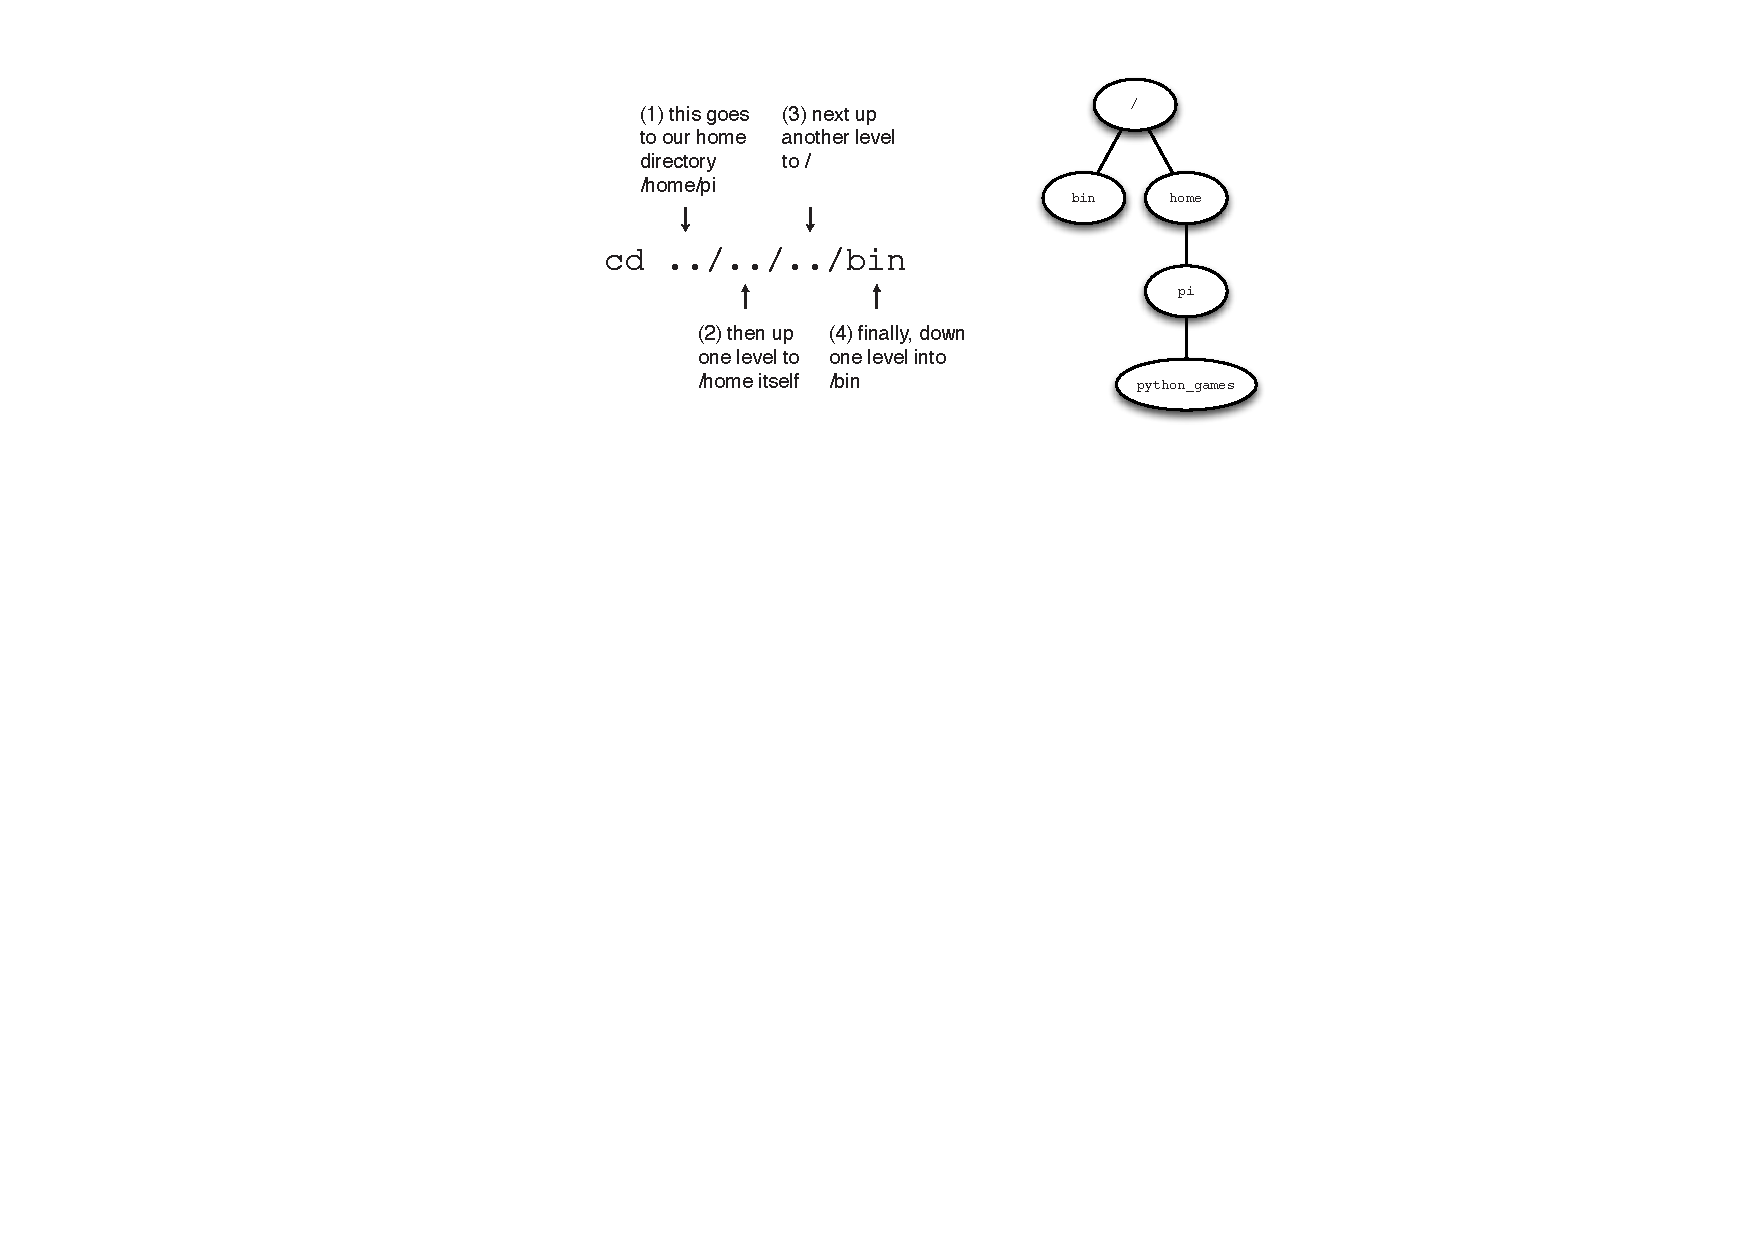
\includegraphics[width=13.5cm]{images/simple-navigation}}
\caption{Given the Pi's default filesystem structure, starting in the \fname{python\_games} directory, the command \fname{cd ../../../bin} will take you to the \fname{/bin} directory (by an admittedly tortuous route!)}\label{figure:simple-navigation}
\end{figure}

%\FloatBarrier
\section{The Colossal Cave}

We're now going to explore a bit of computing history, and install and play one of the very early computer games. Colossal Cave Adventure was the first `adventure game', in which a virtual world is described using only text, and the player controls the game's protagonist using simple textual commands. The game was created in 1976 by a keen caver called \wikipedia{William_Crowther}{Will Crowther} who at time was a programmer at Bold, Berenek \& Newman, the company that developed \wikipedia{ARPANET}{ARPANET}, the forerunner to the modern Internet. He later collaborated with \wikipedia{Don_Woods_(programmer)}{Don Woods}, then a graduate student at Stanford University, to create the Colossal Cave Adventure as we would recognise it today. The original version consisted of around 700 lines of \wikipedia{Fortran}{FORTRAN} code and a similar number of lines of data. When running on a \wikipedia{PDP-10}{PDP-10} (see Figure~\ref{figure:cern-pdp-10} for a picture of what one of these machines looked like) would consume around half of the machine's memory. To put this in perspective, the tiny Raspberry Pi computer on your desk has roughly 1000 times as much memory as the PDP-10; it can run Colossal Cave with ease. 

\begin{figure}[t]
\centerline{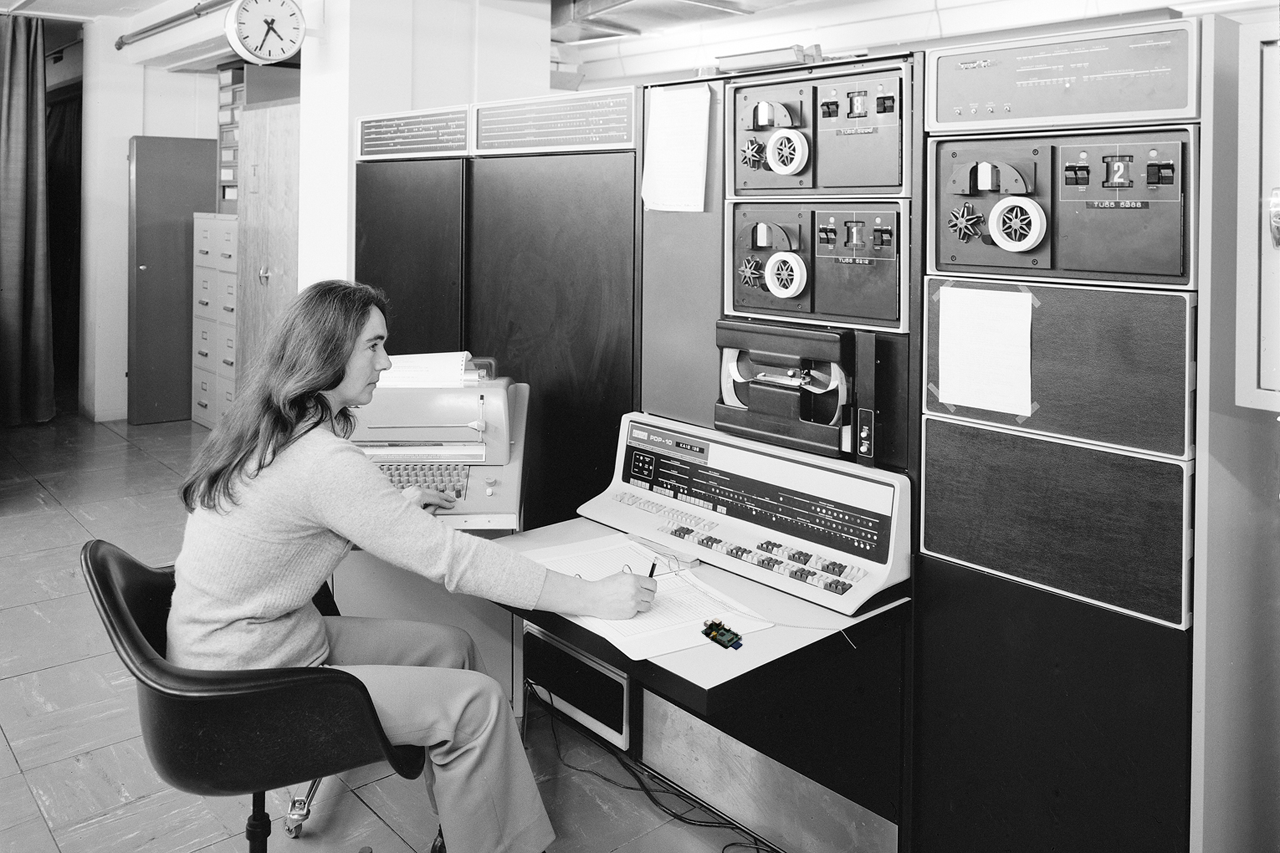
\includegraphics[width=14cm]{images/cern-pdp10+pi.png}}
\caption{A PDP-10 from CERN, circa 1974, reproduced with permission. \url{http://cds.cern.ch/record/916840}. We've taken the liberty of crudely superimposing a Raspberry Pi to approximately the right scale on the operator's desk, just to give a sense of the difference in size between the two machines.}\label{figure:cern-pdp-10}
\end{figure}

Although the original FORTRAN source code for Colossal Cave still exists, the version you're going to play with is based on a re-implementation of the game on what became known as the \wikipedia{Z-machine}{Z-Machine}: a virtual machine specifically for running interactive fiction games.\footnote{Don't confuse the Z-machine, which is a virtual machine for adventure games, with the Z Machine, which is the largest X-ray generator in the world. Doing so is likely to make your lamp melt, and the trolls very grumpy.}
 
\FloatBarrier
\section{Installing Frotz, a Z-Machine Interpreter}

Unlike the other commands that you've used so far, the program we need to be able to play Colossal Cave Adventure isn't pre-installed on the Raspberry Pi, so we're going to have to fetch and install it ourselves. Fortunately, the version of Linux that we have on the Pi comes with a package management system that makes this quite easy. 

But first, we're going to have to understand a command called \totype{sudo}. Everything that you've done so far has involved looking at files that either belong to the `pi' user, or are parts of the system that can be read or executed by any user. But of course, installing a new piece of software involves not just reading, but \textit{modifying} the Pi's operating system in some way, and that's not something that you want to do casually since mistakes could potentially mess up whole device. 

You'll be familiar with the idea of a user with Administrator privileges from Windows or OS X; on Linux the `superuser' that can do anything to any part of the system is called `root' (because this user can modify any part of the system from the root of the filestore downwards). In the early days of UNIX, administrators would log in as the root user to modify, update and repair the system. This had two major downsides: first, that if you accidentally left yourself logged in as the superuser when you nipped out for a coffee, the machine was vulnerable to misuse by anybody who would get at the keyboard; but second and more serious, all the normal safety nets that prevent you from accidentally deleting or damaging the operating system itself are deactivated, so its much easier for a slip of the finger or a brief moment of stupidity to have disasterous effects. To avoid these problems, UNIX systems now usually recommend the use of the \totype{sudo} ('Super User Do') command to temporarily elevate a normal users' privilege that that of super user for a single command. 

The system that we're going to use to install this game is called \totype{apt}, which stands for Advanced Packaging Tool. The \totype{apt} maintains a list of remote \textit{repositories} in which packages have been put that contain all the executables, libraries and data files necessary to install a particular Linux program. It can deal with fetching packages over the Internet, as well as extracting and copying their contents into the right places on your system. It also performs a series of sanity-checks to make sure that what you're adding is compatible what whatever you've already got in place.

The system we want to install to play this game is called \textit{frotz} (to learn why, you'll have to play the game a bit!) Let's try running the \totype{apt-get} command \textit{without} having gained superuser privilege first. Try typing:

\begin{ttoutenv}
$ apt-get install frotz
\end{ttoutenv}

\noindent The operating system will respond with something like:

\begin{alltt}
  \small
E: Could not open lock file /var/lib/dpkg/lock - open (13: Permission denied)
E: Unable to lock the administration directory (/var/lib/dpkg/), are you root?
\end{alltt}

Notice the question at the end: `are you root?'. Well, no you're not, so Linux has rightly prevented you from performing this operation. Now we'll try again using the \totype{sudo} command. This time type:

\begin{ttoutenv}
$ sudo apt-get install frotz
\end{ttoutenv}

You should see a series of lines printed out on the console, ending with:

\begin{ttoutenv}
Setting up frotz (2.43-4) ...
\end{ttoutenv}

\noindent before being returned to the command prompt (note the version number for frotz may have changed from 2.43-4 by the time you use this tutorial, don't worry, that's fine). It's possible that \totype{apt-get} will fail to find the frotz package in one of the repositories it knows about; if this happens, it's usually because the repository has moved somewhere else on the internet, so you need to tell the APT system to update itself first: run the command \totype{sudo apt-get update}, and when that has completed try installing the frotz package again, and all should be well. 

\begin{rpi}{APT}
The APT system is a very convenient way of managing packages, since it will automate the process of finding, fetching, configuring and installing software on your Pi (or indeed, on other Debian-based Linux installations). The RPM system does something similar for distributions based on Red Hat's version of Linux.

The various repositories that contain the packages for your Pi are updated regularly, so it's worth running \totype{apt-get update} once in a while to refresh your Pi's list of software. 

You should also at some point run \totype{apt-get upgrade}, which will cause all the packages that have already been installed to be upgraded to the latest version that the APT system can find. This lab will work just fine with the versions of software that are pre-installed on your Pi, and the upgrade process can take quite some time (hours, possibly), so you mustn't do it now or you won't be able to complete this lab in time. Try it at home, or outside of a lab session. 
\end{rpi}

The frotz system on its own is just a virtual machine into which you can load adventure game data, so we'll need to fetch the Colossal Cave datafile before we can play anything. We've put a copy of the game at \url{http://pod.cs.man.ac.uk/COMP101/Advent.z5} so you can fetch it from there.

Oh, hang on. No web browser. Oh dear.

Although it is actually possible to browse the web in console mode on the Pi (we'll experiment with this in the next lab session), there's an easier way to interact with the web to get the file that we need, using a command called \totype{curl}. First, use \totype{cd} to change to your home directory if you're not there already, then

\begin{ttoutenv}
$ curl http://pod.cs.man.ac.uk/COMP101/Advent.z5 -o Advent.z5
\end{ttoutenv} 

\noindent and you'll see \totype{curl} fetch the file you need `over the web' and save it in your home directory. This is also the first time you've encountered what's called a command-line parameter \textit{switch}: the \ttout{-o} parameter tells \totype{curl} to use the next parameter it sees as the filename for the thing it's fetched from the URL given as its first parameter. More on switches later. 

Use \totype{ls} to confirm that you can see the file \fname{Advent.z5} in your home directory, then type: 

\begin{ttoutenv}
$ frotz Advent.z5
\end{ttoutenv}

\noindent to start playing the Colossal Cave Adventure. Once the game has started (the sceen will have gone blue), type HELP to get instructions. When you've had a bit of a wander around and got the general idea of the game, you can type quit to get back to the command prompt. There's a map of the entire Colossal Cave world at the back of this exercise.

Earlier, we referred to Colossal Cave as a work of Interactive Fiction (IF). In truth, this is perhaps stretching the term somewhat, since the genre has matured considerably in the decades since this first adventure game. For a much more compelling example of Interactive Fiction with beautifully written prose, and funny and challenging puzzles we suggest you have a go at playing Curses by \wikipedia{Graham_Nelson}{Graham Nelson}, or one of the many other games written by Interactive Fiction enthusiasts that are available for free from \url{www.ifarchive.org}. If you find yourself getting hooked on playing IF, the frotz interpreter is available for most platforms, including iOS, Android, OS X and Windows. 

We'll finish this lab session off with one more game. 

Use {\tt curl} to fetch the file hosted at \url{http://pod.cs.man.ac.uk/COMP101/quake3.tar.gz}, making sure you save it in your home directory. 

Notice that this file ends with \fname{.tar.gz}. The \fname{.gz} suffix tells us that this file has been compressed using a utility called \totype{gzip}, so the first task is to uncompress the file. Type:

\begin{ttoutenv}
$ gunzip quake3.tar.gz
\end{ttoutenv}

This will uncompress the file, removing the \fname{.gz} and leaving you with \fname{quake3.tar}. A `tar' file a bundle of individual files that have been assembled together into a single file for convenience. The name `tar' is an abbreviation of 'Tape Archive', since the \totype{tar} command was originally used for making backups of filestores onto tape. It remains, however, a very versatile way of bundling up lots of things, and you'll find tar files all over the internet. 

To see what's in this archive, run the command 

\begin{ttoutenv}
$ tar tf quake3.tar
\end{ttoutenv}

\noindent and you'll see a long list of the archive's contents scroll past on the screen. The first parameter to \totype{tar} is a bit of an odd one, since it's a collection of options, which unusually for UNIX are not prefixed by individual minus signs (recall the \ttout{-o} option we used for \totype{curl}; that's a far more common way of specifying options to tools). In this case the options mean:

\begin{itemize}
\item the \textbf{t} causes \totype{tar} to list the `table of contents', for the archive, without extracting anything.
\item the \textbf{f} tells tar that the next parameter is the file containing the archive. 
\end{itemize}

\noindent To actually extract the contents of the archive we issue the command:

\begin{ttoutenv}
$ tar xvf quake3.tar
\end{ttoutenv}

\noindent where

\begin{itemize}
\item \textbf{x} means `extract'.
\item \textbf{v} means `be verbose, and show what you're extracting as you do it'.
\item \textbf{f} again means `and here is the file to work on'.
\end{itemize}

\noindent When tar has finished working you're presented again with the command prompt. Use \totype{ls} to confirm that you now have a directory called \fname{quake3} in your home directory. Now disconnect the mouse from the desktop PC, and plug it into your Pi; like the keyboard, it's connected to an inline USB socket so you don't need to rummage around behind the computer---and again, please remember to re-attach it to the main PC when you're done here. You might also want to plug some headphones into the Pi at this point too, if you happen to have a pair with you. 

\begin{ttoutenv}
$ cd quake3
$ ./ioquake3.arm
\end{ttoutenv}

\noindent After the startup screen, the game will ask you for a code, but you can just skip this and use the mouse to select the play option. The rest, we're sure, you can figure out for yourself. 

\begin{diversion}{Multiplayer Quake?}
You can play this version of Quake3 Arena with friends over the network. We'll leave you to figure out how to configure that yourself (hint: the \totype{ifconfig} command will tell you what IP address has been allocated to your Pi).
\end{diversion}. 

\FloatBarrier
\section{RTFM}

Although we've introduced several UNIX commands in this lab, we've only done so quite superficially today, giving you just enough detail to get through the tasks in this tutorial. Each of the commands is much more powerful than what you've been exposed to so far. Though you won't need to know every possible option off by heart, there are a lot of useful things you can learn about them quite easily. 

Most UNIX systems, including the one on your Pi have an instruction-manual system that gives more details about the available commands (and most things that you install yourself, such as \totype{frotz} also install their own manual pages).  Try running:

\begin{ttoutenv}
$ man ls
\end{ttoutenv}

\noindent for information on the \totype{ls} command, and use the same trick to find out more about the other commands you've seen today. If you need more help on how to use the \totype{man} command, you can always use: 

\begin{ttoutenv}
$ man man
\end{ttoutenv}

\noindent When you're looking at a manual page, pressing the Space Bar will advance you on a page, and the Up and Down cursor keys will move you back and forth line-by-line.

\begin{diversion}{RTFM?}
The acronym RTFM stands for Read The Flipping Manual, and is sometimes used as a response when somebody has asked a lazy question on a forum or by email where decent documentation already exists and is easily accessible. The F is usually interpreted as meaning something less polite than `Flipping'. 
\end{diversion}

\FloatBarrier
\section{Shutting down your Pi safely}
\label{section:shutdown}

When you're finished playing Quake, exit the game and get back to the command prompt. Like any other computer, its really important that you shut your Pi down properly; if you just pull the power chord out there's a chance of corrupting the filesystem. To shut the Pi down safely, type:

\begin{ttoutenv}
$ sudo halt
\end{ttoutenv}

\noindent You'll see the a series of messages scroll past that look rather like those you saw during the boot process. This shouldn't be surprising, since what the operating system is doing now is shutting down all the things that it started up when you booted the machine, roughly in reverse order. When all these services have closed down tidily, the Pi will power itself down; the network
 and OK LEDs will go off, the screen should go black, and only the red PWD LED will remain lit on the circuit board. At this point its safe to pull the Micro-USB cable out of the Pi. 

\FloatBarrier
\section{What have you learned?}

It might seem like you've been playing games for most of the lab, but if you've followed the instructions carefully and read through all the text you'll have learned a lot of new things. These include:
\begin{itemize}
\item the anatomy of a pi
\item how to safely start and stop your Pi
\item running commands: tar, cd, ls, pwd, unzip, sudo
\item how the filestore is structured
\item basic apt commands
\end{itemize}

\begin{table}
\begin{tabular}{lp{12cm}}
\hline
Directory & Description\\
\hline
boot & Contains the Linux kernel and other low-level packages needed to get the Pi to boot.\\
& \\
bin & Contains the binary executables for basic commands such as \totype{ls} and \totype{pwd}.\\
& \\
dev & This is a virtual directory that represents devices connected to the Pi as though they were files that you can read from and write to. \\
 & \\
etc & Contains configuration files used by various programs, and also the names and encrypted passwords of users\\
 & \\
home & Each user gets their own subdirectory of \fname{home}. \\
 &\\
lib & This is where \textit{libraries} are stored; these are bits of code that are shared between several programs.\\
 & \\
lost+found & If something bad happens and the system crashes half way through doing something, it will put a copy of files that it knows are in a broken state here.\\
media & When you mount removable storage devices such as USB memory stickets, they will appear as filesystems here.\\
 & \\
mnt & This directory is used to mount storage devices. \\
& \\
opt & When you install optional software that's not considered part of the operating system, it usually ends up here.\\
& \\
proc & Like dev, this is a virtual directory. This one contains accounting information about the various processes that are running on your Pi.\\
& \\
selinux & Contains utility files relating to Security Enhance Linux.\\
& \\
sbin & This contains special executable binary files associated with system maintenance.\\
& \\
sys & Various files needed by the operating system.\\
& \\
tmp & Many programs need to create temporary files as part of their execution; they go here, and get deleted when the system reboots.\\
& \\
usr & User-accessible programs and bits of configuration.\\
& \\
var & Another virtual directory, used by programs to store variables.\\
\hline
\end{tabular}
\caption{Standard Linux system directories.}\label{table-dirs}
\end{table}

\clearpage
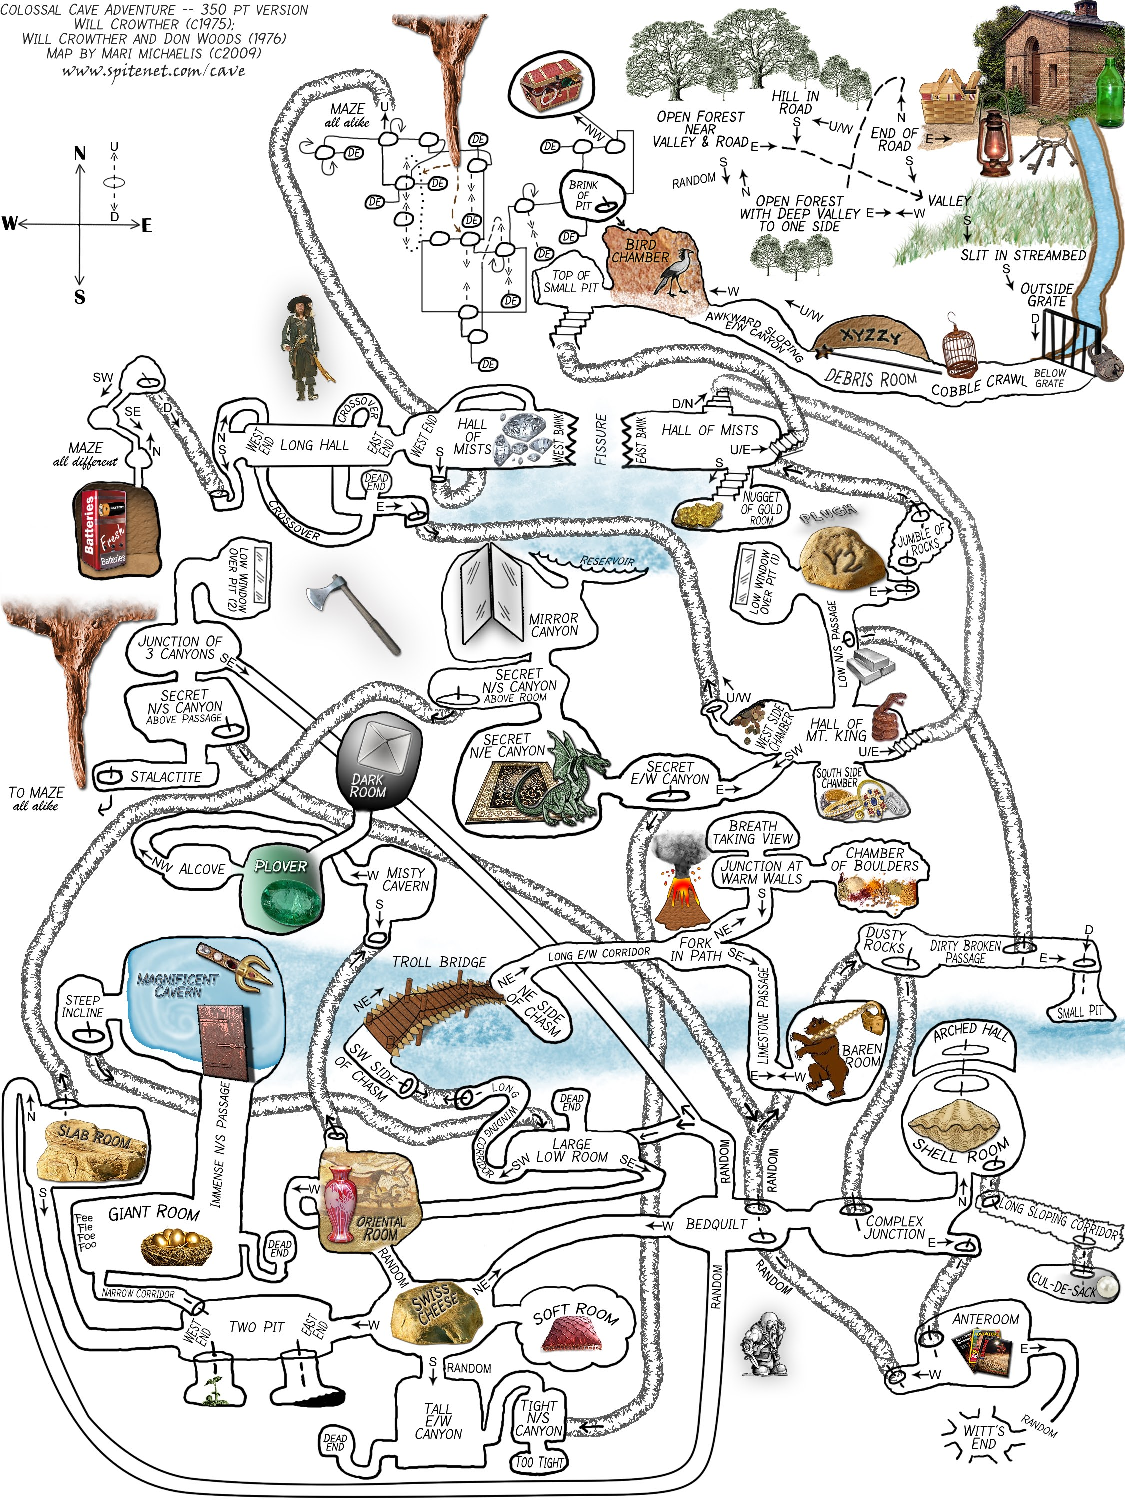
\includegraphics[width=15cm]{images/ColossalCaveAdventureMap}\\
\\
This map of Colossal Cave is reproduced here by kind permission of its author, Mari Michaelis. This is the `spoilers' version of the map, and contains clues as to how to solve the various puzzles in the game. If you want to play the game for real, you probably should make your own map, or at least use the spoiler-free version of the map available at \url{www.spitenet.com/cave}.

%\printbibliography


\chapter{Using the Linux desktop in CS}

Today we're going to explore some of the features of UNIX in a bit more depth, this time using the desktop PCs rather than your Raspberry Pi (we'll return to using that in the next lab). We'll explore some of the more advanced features of the command line and various useful tools that will help you understand how a typical UNIX system is organised. Almost everything that you learn today using Linux on the desktop machine is equally applicable to the Raspberry Pi, and vice versa. 

\section{Reading email in a console}

You're probably familiar with reading email using either a web-based interface, a graphical desktop application (such as Outlook, Thunderbird or OS X Mail) or using an app on a smartphone or tablet. Today you're going to do something slightly different, and configure a text-based mail client so that you can read your university email when logged into Unix at a console. The email client we're going to use is called Mutt, which is fairly simple to configure and straightforward to use (according to its author, Michael Elkins, ``All mail clients suck. This one just sucks less''). There are plenty of other similarly lean text-based \wikipedia{List_of_email_clients}{email clients}, and you may at some point want to check out Alpine as a sensible alternative to Mutt or for the historically-curious, Elm (if you want a \textit{really} hardcore console-mode experience of mail, look up \wikipedia{Mailx}{Mailx}).

First, let's confirm that Mutt is actually installed. Make sure the desktop PC is booted into Linux, and log in using your University username and password (not the username and password you used on the Pi). You should be greeted with a similar command prompt to the one you saw in the previous lab.

To see if Mutt is installed and is accessible to you, type

\begin{ttoutenv}
$ which mutt
\end{ttoutenv}

This should respond with \fname{/usr/bin/mutt}, telling us that the \fname{mutt} command has been put in the \fname{/usr/bin} directory on our system. Remember in the last sessions we looked at the contents of the \fname{/bin} directory that contained essential low-level commands such as \ttout{ls}? Well \fname{/usr/bin} contains commands that aren't quite as essential, but have been installed for the users' benefit (i.e. the system would boot/work without them, but it just wouldn't be very useful.)

List the contents of \fname{/usr/bin} by typing
\begin{ttoutenv}
$ ls /usr/bin
\end{ttoutenv}

and notice that here we're using \ttout{ls} to look at the contents of a directory other than the one we're currently in by passing the directory name as a parameter. A whole load of things should scroll past on the screen; most of them won't mean anything to you right now, but don't worry, we'll look at some of the important ones soon enough. Now that's a lot of stuff to look through, and depending on the size of your screen the command we're looking for may have scrolled off the top. So let's try to narrow our results down a bit. Type 
\begin{ttoutenv}
$ ls /usr/bin/m*
\end{ttoutenv}

and you should be given a much smaller list of things from the \fname{/usr/bin} directory; only those starting with the letter m. The asterisk symbol is interpreted as being a `wildcard' that stands for `anything of any length, including length zero', so the command you've just typed means `list the contents of the \fname{/usr/bin} directory, showing only files that start with the letter m and then are followed by zero or more other characters' (notice that the \ttout{man} command that you used in the last session is there amongst the results). 

You could narrow this down even further by typing \ttout{ls /usr/bin/mu*}, in which case you'll only get files from \fname{/usr/bin} that start with the letters mu. Note that if you leave off the asterisk from your command, you'll be asking for files that are called \textit{exactly} m or mu. 

So far we've been getting you to do a fair amount of typing, and now we have to admit that you've been typing a lot more than you actually need to (it's good practise though, so we're not feeling too guilty at this stage). The default Linux command line has a feature similar to autocomplete that you'll have seen on web forms and in graphical tools, that saves you typing full commands by suggesting possible alternatives. 

Type \ttout{ls /} but don't hit Enter, and instead press the Tab key twice. You'll be shown a list of sensible things that could follow what you've typed---in this case it's the list of directories that are in the system's root. Now type the letter u (so that the line you've typed so far should read \ttout{ls /u}) and hit Tab once. This time your command will be expanded automatically to \ttout{ls /usr/} since that's the only possible option. Press Tab twice now, and you'll get shown the contents of \fname{/usr/}. Type b, and press Tab to expand the command to \fname{/usr/bin/}, and then press Enter to execute the command.

The `autocomplete' function you're using here is more commonly called `tab complete' by UNIX users. If you press Tab once and there's only one possible option that would autocomplete what you've typed so far, then that option gets selected; if there are multiple possible things that could complete your command, then pressing Tab a second time shows you those, giving you the option to type another character or two to narrow down the list. Learning to use this will save you a lot of typing, because not only does it reduce the number of characters you type, it also helps you browse the options/files at the same time. 

Here are some other very useful command line tricks:

\begin{itemize}
\item You can use the up and down cursor keys to cycle back and forth through the list of commands you've typed previously.
\item The left and right cursors do what you expect, and move the insertion point back and forth. Pressing \ctrl{a} will move you to the start of the line, and \ctrl{e} to the end of the line (much faster than moving backwards and forwards character-by-character). 
\item \ctrl{c} aborts the current line, so if you've typed a line of gibberish, don't waste time deleting it one character at at time, just \ctrl{c} it!
\item Typing \ttout{history} lists all the commands you've typed in the past, useful if you've forgotten something.
\item Pressing \ctrl{r} allows you to retrieve a command from your history by typing part of the line (e.g. if you searched for `whi' now, it'll probably find the `which mutt' line you typed a while back). 
\item Pressing \ctrl{t} swaps the two characters before your cursor around. What, really? Yes: you'll be surprised how often you type characters in the wrong order! 
\end{itemize}

Back to configuring your email client. Before we use mutt, we need to point it at the incoming and outgoing email servers, and we'll do this by creating a configuration file.

We've created a template file for you to get going with. Make sure you are in your home directory, then use the \ttout{curl} command as in the last lab session to fetch the template from \url{http://pod.cs.man.ac.uk/COMP101/mutt-template}. Remember, you're going to need to use a switch parameter to tell \ttout{curl} what it should call the file it's fetched (call it anything you like, but \fname{mutt-template} is a perfectly good name). Let's look at the file to see what's in it. Type

\begin{ttoutenv}
$ more ./mutt-template
\end{ttoutenv}

and you should see the following written to the screen:
\begin{ttoutenv}
BLAH
\end{ttoutenv}

The \ttout{more} command is used to display textual content from files and other sources. The reason that the \ttout{more} command is called more will become clear later. 

\begin{note}
  Should they be using 'more' or 'less'
\end{note}

Don't worry too much about the details of this file for now. If you're already familiar with how IMAP and SMTP work together to provide your email service, then you'll be able to see how what the contents of this template mean; if you're not, don't worry, it'll all be explained in detail in the COMP18112 (Fundamentals of Distributed Systems) course in the second semester. For now, we just need to edit that file to contain your details rather than the fake ones in the template you've just downloaded. But lets play it safe: rather than editing the actual file you downloaded, just in case you make a mistake, let's first make a copy of the file in your home directory. Enter

\begin{ttoutenv}
$ cp mutt-template my-mutt-template
\end{ttoutenv}

Did you type all of that? If so, you've wasted several precious keypresses! You could have typed \ttout{cp mu}, and then pressed Tab to expand it to \ttout{cp mutt-template}, and then added on the \ttout{my-mutt-
template} bit yourself. It's a good habit to get into and will save you a lot of time over the next few years.

The basic form of the \ttout{cp} command takes two parameters, the first being the file you want to copy, and the second being the name of the file that will be created. Confirm that there is indeed a new file in your home directory using \ttout{ls}, and that its contents are what you expect using \ttout{more} (how would you find out what else the \ttout{cp} command could do?). 

To modify the file, you'll need to use a text editor. Type 
\begin{ttoutenv}
$ nano my-mutt-template
\end{ttoutenv}

to invoke the \ttout{nano} editor, and use it to change the text in square brackets the the correct values for you. Although fairly basic, the nano editor has all the features you'll need to make these changes, and helpfully shows you the various keyboard shortcuts to do particular things such as saving and quitting at the bottom of the screen (the caret symbol (\textasciicircum) is shorthand for `ctrl', so \textasciicircum X means '\ctrl{X}').

\begin{itemize}
\item $[$USERNAME$]$ should be replaced with your university user name (which will be 8 characters, and will start with an m). Note you'll need to replace this on the lines with \ttout{imap\_user} and \ttout{smtp\_url}.
\item $[$FROM$]$ should be DUNNO!
\item $[$REALNAME$]$ is just your real name, in whatever way you want it to appear in outgoing emails.
\end{itemize}

When you've made the changes, write the file to your filestore and quit back to the command line. Then use \ttout{more} to confirm that the file now looks exactly as you want it to. 

Now, \ttout{mutt} expects the file containing its configuration information to have a particular name, and that's not \ttout{my-mutt-template}, so we'll need to do something about that. The UNIX \ttout{mv} command is used to rename files or directories (it's short for `move'), so use that to change the name of the file to \fname{.muttrc} by typing

\begin{ttoutenv}
$ mv my-mutt-template .muttrc
\end{ttoutenv}

Rather like \ttout{cp}, \ttout{mv} takes two parameters; but this time instead of making a copy of the file, \ttout{mv} just changes the name of the file given as the first parameter to that of the second. 

Type \ttout{ls} to confirm that the file name has changed as you'd expect. 

Oh. But it's gone! Actually, no, it's still there, but it's just hidden! There's a UNIX convention that files that start with a full-stop symbol don't appear when you type \ttout{ls} in its basic form, because these are normally configuration files that you don't need to see on a day to day basis (the `rc' part of the '.muttrc' name stands for 'resource configuration', another UNIX convention). So to see these files you'll need to add an extra switch parameter to \ttout{ls}. Use the \ttout{man} command to find out what this switch is, and then use the switch to confirm that the \fname{.muttrc} file does indeed exist. 

Using this switch on \ttout{ls} will reveal several other so-called `dotfiles' that have been lurking in your home directory all along. Use \ttout{more} to look at the contents of the one called \fname{.bash\_history} and it should become obvious how the \ttout{history} command, and the `reverse search' function you used earlier work.

If you're confident that you now have a file called \fname{.muttrc} containing the correct configuration, you can now type \ttout{mutt} to start the program. 

It should be reasonably clear how you use \ttout{mutt} to send and receive email; if you get stuck there are plenty of online tutorials to help you out. Send yourself a test email to make sure that everything is working, and when you're confident you've mastered the basics of sending and reading using this tool, drop back to the command line. One thing you should note is that \ttout{mutt} doesn't have its own editor for writing email, so will use \ttout{nano} to compose emails unless you change this to something else in the \fname{.muttrc} file. 

\section{Browsing the Web}

Although you will have experienced The Web so far as a highly graphical system, the technology that underpins it is for the most part text-based, and it is (just about!) possible to browse web pages using a console-mode application. It might seem like an odd thing to do, but there's an important point to be made here, so bear with us.

%and install the \ttout{lynx} package using \ttout{apt-get} (remembering you'll need also to use \ttout{sudo} to get root %privileges). 

%Once the package is installed

Try browsing the School's web pages using \ttout{lynx} by typing

\begin{ttoutenv}
$ lynx http://www.cs.manchester.ac.uk
\end{ttoutenv}

Rather like \ttout{mutt}, the \ttout{lynx} program has just about enough on-screen help for you to be able to browse around a little without any additional instructions from us.  You may find that when you follow some links, nothing very much appears to have happened; but scroll further down the page and you'll see the content that you're looking for.

You'll probably find using \ttout{lynx} an unsatisfying experience: tolerable, and probably okay in an emergency, but not how you'd ideally like to browse the web. And you might be wondering why we've even bothered to get you to try viewing the web through a text-only interface. Apart from the absence of images and videos etc., the main difference between using something like \ttout{lynx} and a regular browser such as Chrome, Firefox, Safari or Internet Explorer, is that you'll notice that web pages have been made into much more linear affairs than when they are rendered in a graphical environment. While you might expect to see the navigation links neatly arranged on the left or top of the page with the main content prominently displayed in the centre, seen through a purely textual interface it's all one big stream of stuff, and its very hard to distinguish between the navigation links and the main content. 

Now consider what the web `looks' like if you are visually impaired or blind and have to use use a screen-reader (a voice-synthesiser program that vocalises the text that's on-screen) to interact with your computer. Whereas a sighted person can easily cope with a two-dimensional layout that allows you to be aware of multiple things at the same time (i.e. you can be reading the main content of the page, but conscious of the fact that there's a navigation bar on the left for when you need it), if instead you are listening to a voice reading the contents of the page out to you, it's only possible to be hearing one thing at a time. And what's more, you have to remember what has been read out in the past in order to make sense of what you are hearing now; you can't just `flick back' a paragraph or two by moving your eyes, instead you have to instruct the screen reader to backtrack and re-read something. So the experience of using the web if you are visually impaired has some things in common to interacting with web-pages using \ttout{lynx}. 

You'll soon be designing your own web-based systems as part of the Group Project in this course unit; making them accessible to visually impaired readers something you should keep in mind. Try using \ttout{lynx} to browse some of your favourite websites, and you'll almost certainly find that the level of `accessibility' on the Web varies considerably!

\subsection{Pipes and Redirects}

One of the fundamental philosophies of Unix -- and one that is a sensible philosophy when you're building any computer system really -- is that the operating system is composed from lots of simple sub-systems, each of which performs one clearly defined task. To do something more complex than any of the individual tools allows you to do on its own, you are expected to combine components yourself. At the command line, Unix makes this quite simple, so let's give it a go. 

First, use lynx to look at the BBC's weather page at \url{http://www.bbc.co.uk/weather} and have a quick browse around to get familiar with what it looks like. Then quit lynx and get back to the command prompt before typing:

Type:
\begin{ttoutenv}
$ lynx -dump http://www.bbc.co.uk/weather
\end{ttoutenv}

Note the addition of the \ttout{-dump} parameter before the URL this time. Instead of running as an interactive browser, \ttout{lynx} should have just dumped the text that it would have displayed for that page to the console, and then quit. Now, most of the text of the page will have scrolled off the top of the screen, so let's use the \ttout{less} command to allow us to page through lynx's output in a more controlled manner. Type:

\begin{ttoutenv}
$ lynx -dump http://www.bbc.co.uk/weather | less
\end{ttoutenv}

Did you type all that? Hopefully not---remember you can use the up and down cursor keys to get previous commands back at the interactive prompt, and then just modify or extend them to save wearing out your fingers.

To explain what's happened here, you'll have to understand the concept of `standard in' and `standard out', which is a neat and extremely powerful idea that is fundamental to the way tools (and programmes generally) work in a Unix environment. 

Unless they are told otherwise, every Unix program has access to two ways of communicating with other parts of the operating system. The first, `standard in' allows a stream of data to be read by the program; the second, `standard out' gives the program a way of displaying textual responses. By default, when you execute things at the command prompt, Unix arranges for a program's standard in to be connected to whatever you type at the keyboard, and for its standard out to be connected to whatever display you're using at the time (this is a bit of an over simplification, but it'll do for now). It's quite easy to arrange for standard in and standard out to be connected up differently though, and that's what you've just done.

The vertical bar `\verb-|-' before \ttout{less} is called the `pipe' symbol, and it is used to join the output of one command to the input of another; so in this case we have connected the standard output from \ttout{lynx} directly to the standard input of \ttout{less} (when \ttout{less} is invoked without a filename argument, it expects to get its input from standard in). 

Instead of joining commands together, you can use the idea of manipulating standard in/out to create or consume files instead. Try:

\begin{ttoutenv}
$ lynx -dump http://www.bbc.co.uk/weather > weather.txt
\end{ttoutenv}

and then use \ttout{ls} to confirm that a file called \ttout{weather.txt} has been created, and use \ttout{less} to look at its contents (which should be just the text from the weather web-page we've been looking at already). Here the \verb-`>'- symbol redirects the standard out of the lynx command so that instead of going to the console display it gets put into a named file. 

To finish off this first contact with pipes and redirects, we'll use a new command called \ttout{grep} along with lynx to create a simple command of our own that tells you what the weather is like in Manchester (there are very few labs with windows onto the outside world in the Kilburn Building, so this may be more useful than you think!) 

Grep is a hugely powerful and useful utility, designed for searching through plain-text files. Learning to master grep will take more time than we have in this lab, since you'll have to understand the idea of \textit{regular expressions} to make full use of it (we'll come to those in \ref{sdjfosdifj}). For now, we'll use it in its very simplest form. Type:

\begin{ttoutenv}
$ grep BBC weather.txt
\end{ttoutenv}

and you should see a list of all the lines from \ttout{weather.txt} that contain the word `BBC'. Use \ttout{less} to have a look for other terms to `grep' for (you might want to try something like `Sunny' to give you a list of all the places where the weather is nice, for example). 

Rather like \ttout{less}, if grep isn't given the name of a file as its last command-line parameter (in this case we used \ttout{weather.txt}), it will operate on standard-input instead of grepping through a file (yes, it's quite okay to use grep as a verb from now, no one will look at you funny). Use this knowledge to join together lynx and grep so that the output is a single line describing the weather in Manchester right now. The output should look something like:

\begin{ttoutenv}
   [33]Manchester 22°C 72°F
\end{ttoutenv}

As a final flourish, let's create a new a way of accessing this new `weather in manchester' tool that you've created. Type:

\begin{ttoutenv}
$ alias mankyweather="[YOUR COMMAND GOES HERE]"
\end{ttoutenv}

replacing [YOUR COMMAND GOES HERE] with the full command line you created to display the Manchester weather. Then try typing

\begin{ttoutenv}
$ mankyweather
\end{ttoutenv}

to see the result. Okay, so this probably won't replace your favourite weather webpage or app, but its early days yet! 


\section{X Windows and Gnome} 

Next you're going to start up one of Linux's many graphical user interfaces. Type:

\begin{ttoutenv}
$ startx
\end{ttoutenv}

You'll see a chunk of text scroll up the screen briefly before being presented with something that looks like the screenshot in Figure \ref{figure:gnome-desktop}.

\begin{figure}[t]
\centerline{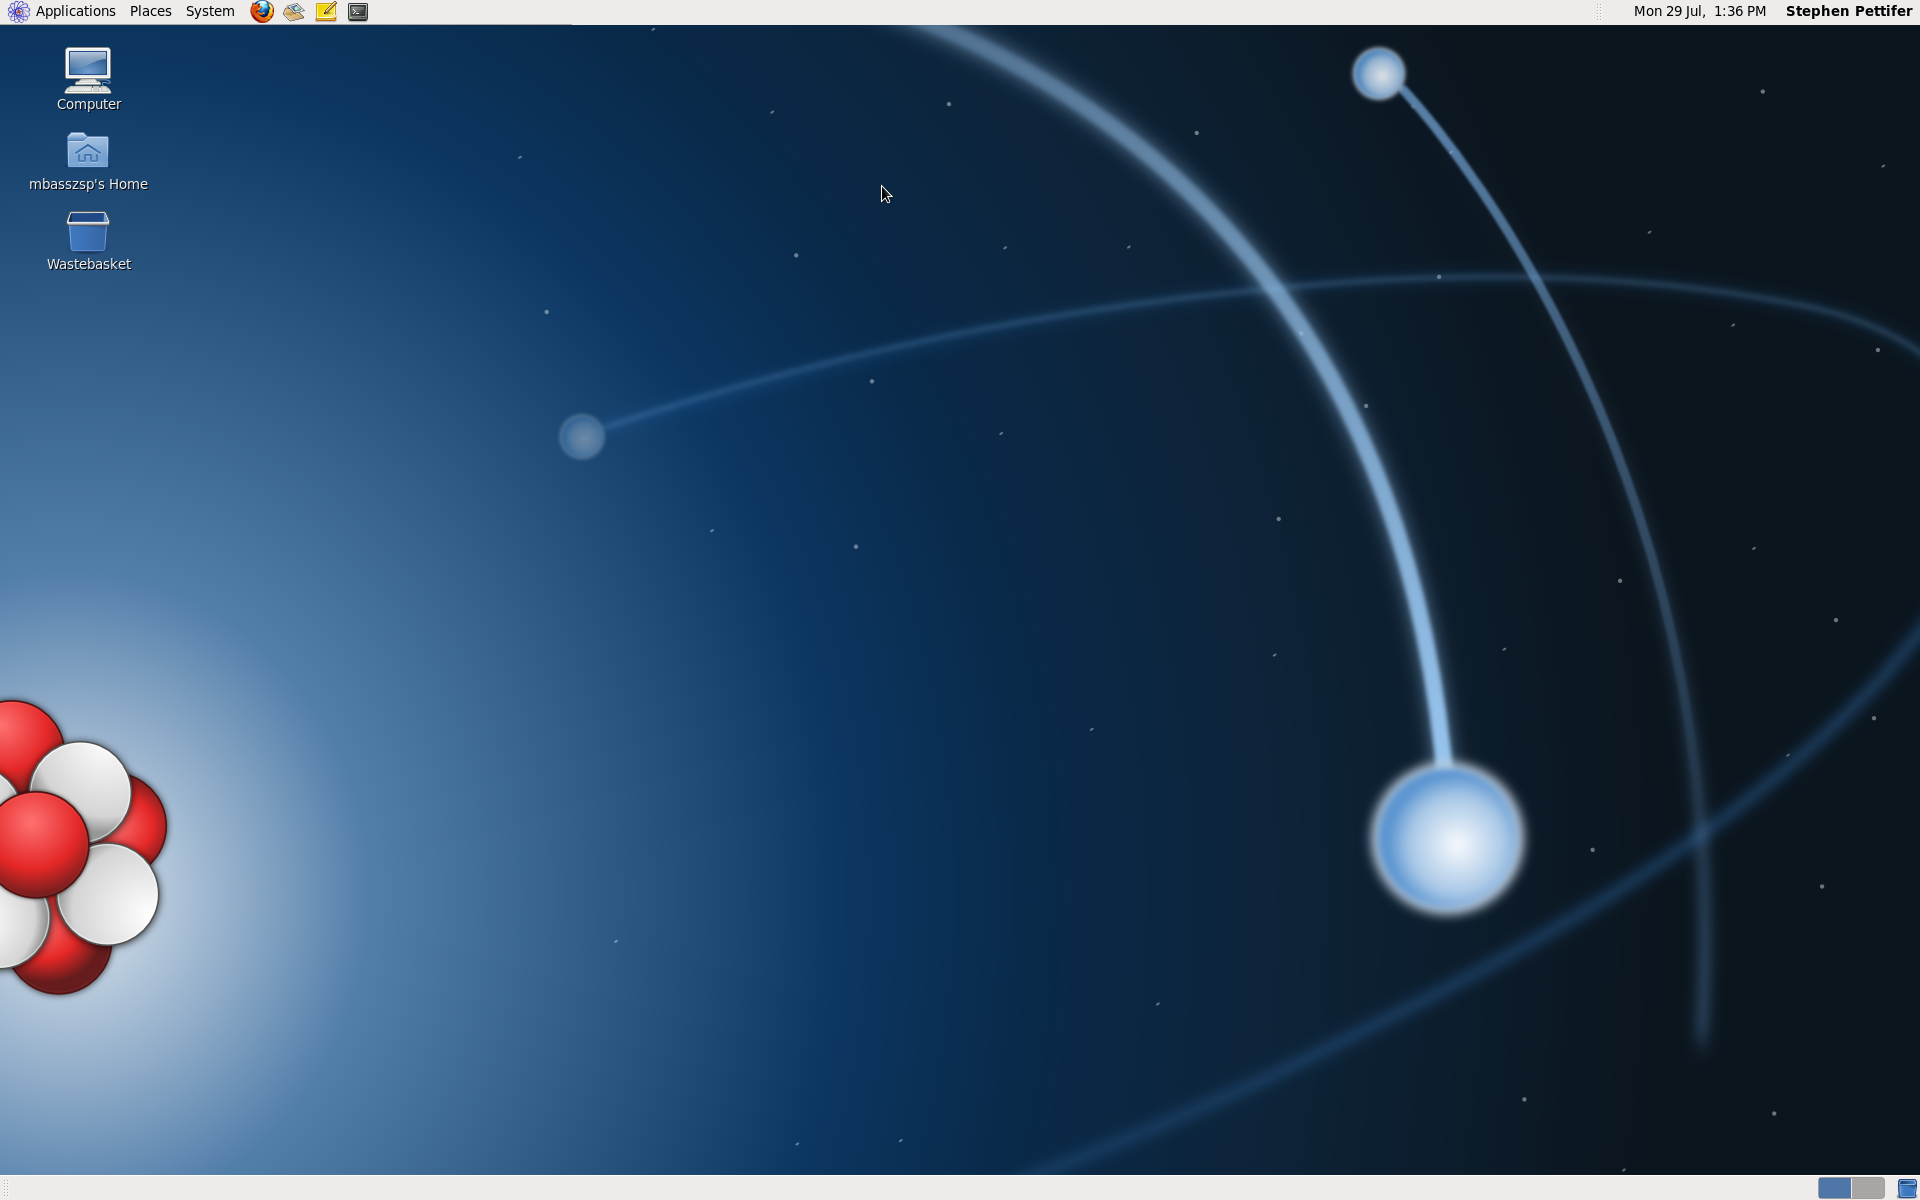
\includegraphics[width=15cm]{images/gnome-desktop}}
\caption{Scientific Linux's default graphical user interface and window manager, Gnome.}\label{figure:gnome-desktop}
\end{figure}

Take a few minutes to explore the graphical environment. Even if you've never used Linux before, you'll probably find the general principles of this environment quite familiar: there are icons on the desktop giving you access to the computer via a graphical file browser, and at the top of the screen a menu-bar allows you to start various applications and utilities. The full manual for this environment --which is called Gnome --is available online at \url{http://personal.us.es/rledesma/descargas/gnome2.6-user-guide.pdf}, but you'll probably be able to work out everything you need to get you going by poking around at the various buttons. Unlike the Raspberry Pi where you have complete control over the operating system via the \texttt{sudo} command, the lab machines are configured so that you can't do any long-term damage to the setup. Apart from accidentally deleting your own files (and right now you have nothing to accidentally delete!), there's nothing much you can do that will cause problems, so feel free to explore a bit. 

Find out how to:
\begin{enumerate}
\item Find two ways of starting the Firefox web-browser.
\item Work out how to change the desktop theme. 
\item Find Application Blahdeblah. \ref{thingyblobbs}
\item Something else, and when you're done with these
\item Figure out how to log out of the graphical environment.
\end{enumerate}

If you've completed step 5 you should now be back at the command prompt where you typed `startx' a little while back. Before returning to the graphical environment where you'll spend most of your time, it's important to understand how the graphical interface you've just been using works as part of the Unix operating system. 

If you remember back to the first Raspberry Pi lab, we pointed out that the \texttt{shell} that you're using to interpret commands is `just a program' that happens to interpret input from the user, execute commands, and display the results. The graphical environment you've just used is similar -- just a program (or actually, collection of programs) that runs on the operating system.

But what do we mean by `execute commands'? You've probably got the hang of the fact by now that most of the things that happen in Unix are just programs stored somewhere on the file system (remember, you found some of them in the \texttt{/usr/bin} directory on the Pi). When you press return at a shell prompt, the program that is the shell checks that what you've typed has a valid syntax, and then starts up a new \textit{process} in which that program executes. The process is mostly independent of the shell program that started it, gets on with doing whatever it was designed to do, and when it finishes it tells the shell that it's done, and the shell gives you another prompt for the next instruction. Something very similar happens when you run the \texttt{startx} command: the graphical environment starts executing, and when you select the `log out' option, it returns you back to the shell so you can issue another command. Notice that you haven't been `logged out' of the machine, but rather just out of the graphical environment. 

Now, if you're going to use the graphical environment as your primary interface (and, as the jobs we ask you to do get more complex, you're going to need to!), you may find it slightly annoying to have to log into a lab machine, start the graphical environment, log out of the graphical environment when you're done \textit{and then remember to also log out of the console environment before you leave (because if you don't do this, other people will have access to your account!)}. 

Type the following:

\begin{ttoutenv}
$ exec ls
\end{ttoutenv}

You should find that the \texttt{ls} command has done exactly what you normally would expect, but that instead of returning you to the command prompt, you've been unceremoniously logged out! Log back in again (sorry about that). 

The \texttt{exec} command changes the way in which the shell deals with whatever command follows it. Instead of starting a new process in which to run your command and waiting in the background for that command to complete, the shell gives up the process in which it itself is running, and hands it over to the command you've issued. So when that command finishes, there is no shell to come back to. And because in this case the shell was the first program that got run when you logged in, the Unix system logs you out since there's nothing else you can do. 

Experiment by running \texttt{exec startx} and then logging out of the graphical environment as you did a moment ago; this time you should find that you've automatically been logged out of the console too.

But although that's one step closer to what we want, there's still the issue of having to type \texttt{exec startx} every time you log in. Of course this isn't a huge deal (it's certainly not as annoying as accidentally leaving yourself logged in at a console), but we can do better than this. 

When you first run the bash shell, it looks for a file in your home directory called \texttt{.bash\_profile} and executes any commands it finds in there as though you'd typed them at the keyboard. Use the \texttt{ls -a} command to confirm that there's already a file in your home directory called \texttt{.bash\_profile}, and then use \texttt{less} to look at its contents.

It should look something like this:

\begin{ttoutenv}
# .bash_profile

# Get the aliases and functions
if [ -f ~/.bashrc ]; then
	. ~/.bashrc
fi

# User specific environment and startup programs

PATH=$PATH:$HOME/bin

export PATH
\end{ttoutenv}

though don't worry if there are slight differences. We'll come back to what these instructions mean a little later one. For now, fire up the \texttt{nano} editor, and use it to add a new line at the end of your \texttt{.bash\_profile} that reads 

\begin{ttoutenv}
exec startx
\end{ttoutenv}

Now log out (either type \texttt{logout} or press Ctrl+D), and log back in again. If all has gone to plan then you should see the graphical environment fire up automatically; and when you select `logout' from the menu, you should be returned to the Linux login prompt. 

Hurray!

\section{A quick tour of Gnome}

\begin{itemize}
\item terminal
\item editors
\end{itemize}

\section{X Windows}

Let's take a step back now and look at what the \texttt{startx} command has actually done. Unlike operating systems such as OS X and Windows, Linux doesn't really `have' a graphical windowing environment `built in'; what you've seen just now is a series of programs that co-operate with one another to give create the familiar WIMP environment. 

\begin{figure}[htb]
  \begin{center}
    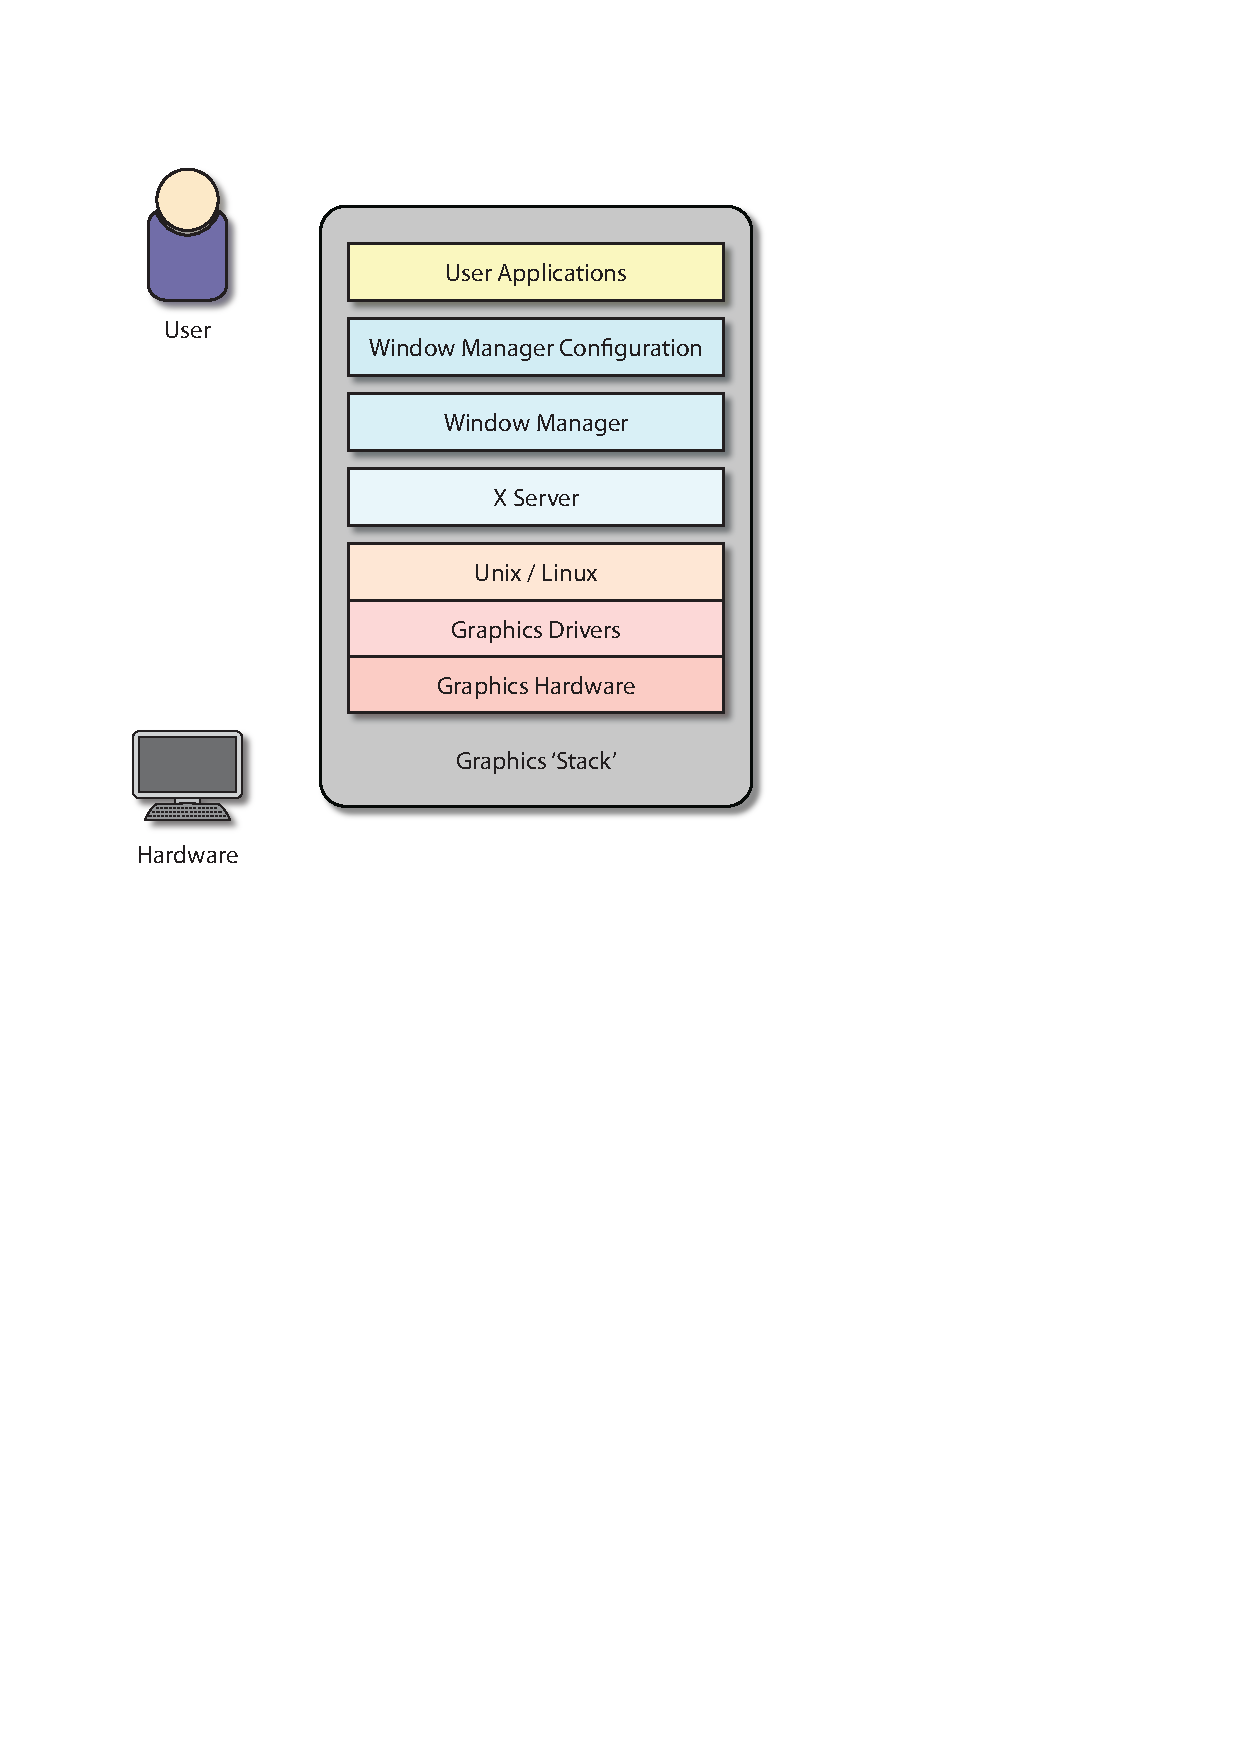
\includegraphics[width=12cm]{images/graphics-stack.pdf}
  \end{center}
\caption{The layered structure of Linux's graphical system, with software nearest to the underlying hardware at the bottom, and software closest to the user at the top.}
\label{figure:Xstructure}
\end{figure}


When you ran Quake and the snake game on the Pi in the previous lab, these programs took direct control of the graphics subsystem in order to display the game. The \texttt{startx} command runs a program called the XServer, which also communicates with the computer's graphics system, but on its own doesn't really do anything very exciting apart from allow other programs to then share the display. Along with the XServer, a window manager (in this case, called Gnome) was started, and this is what you see drawing the buttons and menus and window controls for the graphical user interface. You'll explore the architecture and features of the XServer in a lot more detail in COMP18112 (Fundamentals of Distributed Systems) in the second semester. For now, it's enough to understand that there are two things going on here, first the X Windows system is running that allows things to be drawn on regions of the screen, and second the Window Manager which is doing all the WIMPy stuff like providing all the controls that allow windows to be moved and resized. 

One of the interesting effects of this architecture is that you can use different window managers on Linux, and can choose the one that best suits the way you work. So although in Gnome you can change the theme of the desktop, it's actually possible to replace Gnome with something else entirely. 

To demonstrate this, use nano to create a file in your home directory called \texttt{.xinitrc}, and in that file put a single line that reads:

\begin{ttoutenv}
BLAAAAAAAH
\end{ttoutenv}

%\printbibliography

\chapter{Pi power}
\minitoc
\notesurl{rpi2}

So far you've used your Pi and the lab PCs separately, and hopefully you've come to understand that they are both essentially the same kind of machine; they both run variations of the same operating system, and the principles you learn using one for the most part apply to the other. In the case of the Pi, you have complete control of the device as a superuser, so can do absolutely what you like to it; in the case of the lab machines you have access to much more powerful hardware, but more restricted access to the filestore and operating system for reasons of security and privacy. 

Today, we'll be getting your Pi and a desktop PC to communicate with one another, to reinforce the similarities between these setups, and to expose you to some of the principles of networking and remote access. 

\section{The LXDE window manager}

Connect your Pi up to the monitor, keyboard, mouse, network and power supply as before, and log in (remembering this time to use whatever password you set on the Pi rather than your University password, and the username `pi'). At the console, type:

\begin{ttoutenv}
$ startx
\end{ttoutenv}

to start up X Windows and the Pi's default window manager, LXDE, which appear moments later looking like the screenshot in Figure \ref{figure:lxde-desktop}. 

LXDE (the `Lightweight X11 Desktop Environment') is designed to be a lean, fast desktop environment, which makes it ideally suited for the Pi's modest CPU. Although rather less rich in features and `eyecandy' than Gnome, LXDE is a fully functioning environment that has all the features you will need for operating and programming the Pi. 

Down at the bottom of the screen you will see LXDE's `panel'. On the left of the panel (\protect\circled{1} in the figure) are controls that give you access to various applications, tools and system preferences. On the panel's right (marked \protect\circled{2}) are a CPU meter, a clock, a control that will allow you to lock the Pi's screen temporarily so that you can nip out for a coffee, and the logout button that does what you'd expect a logout button to do (though remember--it's just going to log you out of the windowing environment, and not log your user out of console mode; we explained how you could do that using \cmnd{exec}{exec} in the previous lab session). On the desktop itself are shortcuts to some useful applications including a Terminal and Midori, which is a simple web browser. 

Spend a few minutes exploring the GUI. You'll may find that you're double-clicking on things that only need a single click, and vice versa, and may find that things aren't quite where you expect them to be---but rather than dismissing LXDE as being crude, embrace the differences; you may well find that you come to prefer its `no frills' approach to window management over that of richer, heavier-weight environments such as Gnome. LXDE and other slimmed-down graphical environments consume considerably fewer CPU cycles and hence less power than their richer counterparts, and while this isn't an issue when you're running on a mains-powered desktop machine with a reasonably beefy graphics card such as the lab PC, this can be a serious issue for devices running off batteries. 

\begin{figure}
\centerline{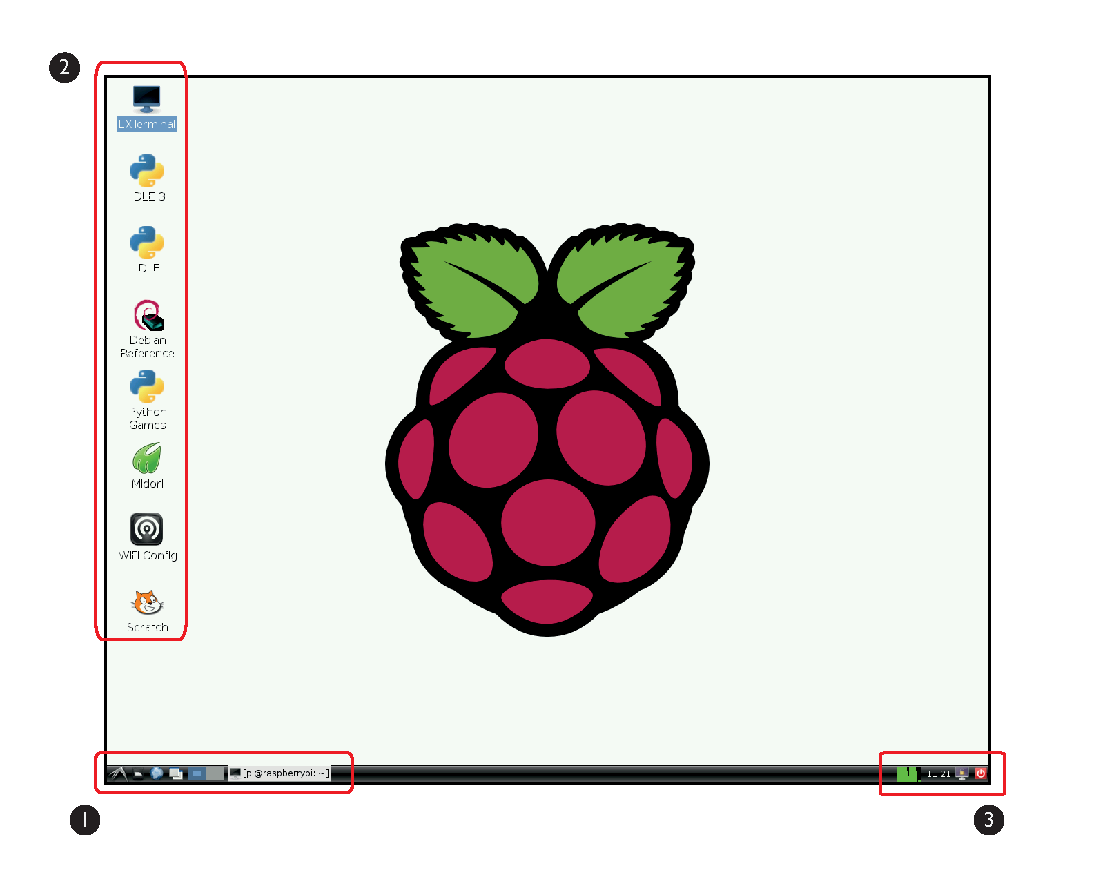
\includegraphics[width=14cm]{images/lxde-desktop}}
\caption{The Pi's default window manager is called LXDE.}\label{figure:lxde-desktop}
\end{figure}

\section{Configure mutt}

Once you've found your way around LXDE, fire up a terminal so that you can configure your Pi to read your University email using \cmnd{mutt}{Mutt}. Unlike the lab machines, \cmnd{mutt}{Mutt} isn't installed by default on the Pi, so you'll need to do that yourself using:

\begin{ttoutenv}
$ sudo apt-get install mutt
\end{ttoutenv}

Once the install has completed, you'll need to adjust Mutt's settings so that they once again point at your University email account. You could do this by following the instructions in the previous session's script again, but there's a much easier way: let's just copy the configuration file you created on the desktop PC last time, over to the Pi. 

First you need to check that you still have the \fname{.muttrc} configuration file in your home filestore of your Computer Science network account. You \textit{could} unplug all the cables from the Pi, connect them back into the desktop PC and check that way, but that's no fun (especially because we'd then have to reverse it all to do the next bit of the exercise). But you don't need to do that--you can check \concept{remotely}. 

\begin{note}
Picture of the hostname sticker, and update this with new new hostname style
\end{note}

So, find the hostname of the lab PC on your desk; there should be a sticker on both the PC itself and the monitor with a name such as `E-C07KILF3101'. If for some reason there isn't a sticker, there are several ways you can find out the hostname (you'll need to switch the monitor back to the DisplayPort input, and may also need to re-attach the keyboard/mouse usb lead to the desktop PC):

\begin{itemize}
\item If you haven't logged into the PC, then it should be showing a login prompt like  \ttout{E-C07KILF3101:}
\item If you're already logged in, but have not started a window manager, your console prompt will be something like  \verb|[mrnoodle@E-C07KILF3101 ~]$| (where \ttout{mrnoodle} would be replaced by your own username, of course).
\item If you are logged in to the PC and inside a window manager, open a terminal window. It should show you the command line prompt, as above. You could also type \verb|echo $HOSTNAME|.
\end{itemize}

Once you've got hold of the PC's hostname, we're going to use a \wikipedia{Secure_Shell}{Secure Shell} to connect to from the Pi to the the desktop, allowing you to type commands on the Pi that will be executed remotely via a shell that's executing on the desktop PC. In the terminal window on the Pi, issue this command:

\begin{ttoutenv}
$ ssh [USERNAME]@[HOSTNAME].cs.man.ac.uk
\end{ttoutenv}

replacing [USERNAME] with your University username, and [HOSTNAME] with the name of the PC in front of you. You'll need to enter your University password, and will most likely be presented with text something similar to this:

\begin{ttoutenv}
The authenticity of host 'E-C07KILF3101 (130.88.197.112)' can't be established.
RSA key fingerprint is 20:6d:2d:90:5e:8f:9f:19:39:70:ce:48:a6:93:ec:4c.
Are you sure you want to continue connecting (yes/no)? 
\end{ttoutenv}

Type \ttout{yes} (and hit enter) in response to the question. You should then be given a command prompt (you'll learn more about what this message actually means in \courseunit{COMP18112}, but for now just treat it as something that happens the first time you try to connect to a particular machine). Notice that this command prompt no longer says \ttout{pi@raspberrypi}, but rather has the name of the machine you've just remotely logged into. 

Type \cmnd{ls}{ls -a} to confirm that your \fname{.muttrc} file is still where you expect it to be, and if all is well then press \ctrl{D} to log out of the remote shell you just started, and you will return to the shell running locally on your Pi (you'll see the command prompt change back to being `pi' again). Now we know the file we want is there, we need to copy it from your Computer Science filestore onto your Pi's local filestore.

To do this, we're going to use the \cmnd{scp}{scp} (Secure Copy) command, which in some ways behaves like \cmnd{cp}{cp}, but allows us to move files \textit{between machines}. 

Like \cmnd{cp}{cp}, the \cmnd{scp}{scp} command in its basic form takes two arguments, the first is the name of the source file (the one you want to copy), and the second is the name of the destination file (the one you want to create). The difference with \cmnd{scp}{scp} is that either (or less commonly, both) of these files can be on a remote machine, which means that you need to provide the command with enough information about the location of the remote file in terms of the hostname and file system, and any login details necessary to get at it. The syntax for providing this information is:

\begin{ttoutenv}
[USERNAME]@[HOSTNAME]:[FILEPATH]
\end{ttoutenv}

So for example, if you wanted to retrieve a file called \fname{cheese.jpg} from the home directory of a user called \ttout{mrnoodle} that was stored on a machine with the hostname \ttout{mypc.example.com}, and you wanted the local copy of the file to be called \fname{mycheese.jpg} the command would be:

\begin{ttoutenv}
$ scp mrnoodle@mypc.example.com:cheese.jpg mycheese.jpg
\end{ttoutenv}

Then, supposing you had edited the file \fname{mycheese.jpg} on your local machine and wanted to put the file back into the home directory of the \ttout{mrnoodle} account on the remote machine, but under a different name (so as not to over-write the original), you would use the command:

\begin{ttoutenv}
$ scp mycheese.jpg mrnoodle@mypc.example.com:newcheese.jpg
\end{ttoutenv}

We're not exactly sure why MrNoodle and cheese feature quite so prominently in these labs either, just go with the flow. Now use your new-found knowledge of \cmnd{scp}{scp} to copy the \fname{.muttrc} file from your Computer Science account onto your Pi. Conveniently, there's nothing in the \fname{.muttrc} file that is specific to the Computer Science account setup, so you can use it as-is for Mutt on the Pi (as usual, if you get stuck as for help.)

Check that the file has copied over successfully using \cmnd{less}{less}, and then start up \cmnd{mutt}{Mutt} from a terminal. If everything has gone to plan, you should now be able to read and compose emails on your Pi. You can of course install other mail clients if you want to; there is a version of Thunderbird for the Pi called Icedove (yes, yet another play on words), or a much leaner graphical client called Claws Mail (which if you want to can be installed using \ttout{sudo apt-get install claws-mail}). Remember, though, that the memory-card we've given you for your Pi is fairly small, so you probably don't want to clutter it up with unnecessary packages, and you should find that Mutt is perfectly okay for sending and reading the occasional email. 

\subsection{Emailing your tutor}

To test that you've sucessfully set \cmnd{mutt}{mutt} up on the Pi, use it to send a friendly email to your tutor to tell him or her that you're reached this point of the lab . If you've not figured out your tutor's email address yet, you can find it at
\\
\url{http://www.cs.manchester.ac.uk/aboutus/people/}

\section{X Windows again}

As we mentioned before, the X Windows system is a powerful beast, and although it was designed a long time ago (around 1984), it was in many ways way ahead of its time--rather like the design of Unix itself.

Remember that the GUI you're now using on the Pi consists of two systems working together: X Windows (which amongst other things gives software access to the display hardware), and the Window Manager (in this case, LXDE) that provides the WIMP-style features such as movable windows and clickable controls. The X Windows system operates as a Client/Server architecture, where the `server' part does the drawing of stuff onto the screen, and clients request that things be drawn. One of the really nice features of X Windows is that it doesn't care too much about where the requests to draw things come from. Typically they come from processes that are running on the same computer as the X Server, but this need not be the case as you're about to demonstrate.

Log back in to the lab PC using the \cmnd{cmnd}{ssh} command, but this time include a \texttt{-X} switch before your username, like:

\begin{ttoutenv}
$ ssh -X [USERNAME]@[HOSTNAME]
\end{ttoutenv}

The \ttout{-X} switch (note that it's an uppercase X) tells the \cmnd{ssh}{ssh} program to send any X Windows graphics generated on the remote generates back through the network from the remote machine to the X Server running on the local machine.

\begin{note}
Fix / simplify the above
\end{note}

Confirm that you are indeed logged into your Computer Science account by checking the command prompt and using \cmnd{ls}{ls} to make sure the files in your home directory are the ones you'd expect, and then type:

\begin{ttoutenv}
$ xeyes
\end{ttoutenv}

Googly eyes that follow the mouse! What's not to like? Well, okay, perhaps not hugely exciting in itself, but what's actually happening here is rather interesting and quite sophisticated. The \cmnd{xeyes}{xeyes} program is running on the remote machine (the desktop PC); but the instructions to draw its graphical output are being forwarded over the secure shell connection you've made from the Pi to the remote machine, so that the Pi's X Windows system receives them. Press \ctrl{C} to quit \cmnd{xeyes}{xeyes}, and instead try running \cmnd{xterm}{xterm}. You should see a new terminal window appear on your Pi's screen (which probably looks slightly different to the terminal you launched on the Pi a moment ago; it does essentially the same thing though). This X Terminal, rather like \cmnd{xeyes}{xeyes}, is actually running on the desktop machine---only its graphical representation is appearing on your Pi (if you use \cmnd{ls}{ls} in that terminal, you'll see that its your Computer Science account that's visible, rather than your Pi's filestore and you can confirm this another way using the \cmnd{hostname}{hostname} command). 

%How could you use this feature to your advantage to give you a temporary graphical mail client (or perhaps to use Firefox as a web browser, rather than Midori) on the Pi without needing to install any packages on the Pi itself? 

\begin{note}
may need a diagram to help explain what's going on here
\end{note}

\section{A Simple Web Server}

This next exercise involves setting up a simple web server on the Pi, but before we can do that you'll need to create some basic web pages to display. 

\begin{note}
fix this bit
\end{note}

Start up a terminal, and use the \cmnd{mkdir}{mkdir} to create a directory called \ref{FIXME} your home directory, and in that directory, use \cmnd{nano}{nano} to create a file called \fname{index.html} with the following content:

\begin{ttoutenv}
<html>
<body>
Hello world!
</body>
</html>
\end{ttoutenv}

From within that directory, run the command:

\begin{ttoutenv}
$ python -m SimpleHTTPServer
\end{ttoutenv}

and then use Midori to browse to the following URL:

\begin{ttoutenv}
http://localhost:8000
\end{ttoutenv}

If your browser displays a page saying `Hello World', pat yourself on the back---you've just created a web page \textit{and} set up a simple web server to host it. The URL you used to view this page may look a bit odd compared with others you have seen. The \texttt{http://} part you'll no-doubt be familiar with from other web-addresses that you've seen; the `localhost' part is a convention that means `this machine'. The section of the URL that follows \texttt{localhost} may be even less familiar: this is the \textit{port} (communication channel) on which the simple web-server that you've set up is serving web pages; by default web browsers expect servers to use port 80, but the \ttout{python -m SimpleHTTPServer} command you used here defaults to port 8000, so we had to add that to the URL. We'll leave the issue of ports there for now, and revisit that in more detail in the 2nd semester in \courseunit{COMP18112}. 

\subsection{A slightly more interesting web page}

\begin{note}
give them a default MrNoodle Webpage
\end{note}

Now spend a few minutes modifying \fname{index.html} to create a slightly more interesting web page. Create a single page about yourself that contains a paragraph describing who you are, which programme you're on (e.g. Computer Science, Software Engineering, etc.), and which contains a picture of yourself as well as the image you created in the previous session using Inkscape.

Don't worry about finely crafted words here---this is really just a way of creating a file that we can get you to edit in various ways a little later on. A few sentences will do, and you can always change it later. 

As for the photograph of you, we'd ideally like you to use something recent that someone could recognise you by, but it doesn't really matter too much: it can be any kind of photo you like; silly or serious, whatever you're comfortable with, but please make sure it doesn't contain anything offensive. If you're not comfortable with having a photo of yourself on the net, you can use a photo of something else (but you must make sure you have permission to re-use a picture that's not yours; anything you find on Wikipedia should be okay for this purpose, and there will be more guidance on how to use others' photos later in this course). If you didn't have a photo handy, take one with your phone, or ask one of your fellow students to do it for you on theirs.

You've already learned several ways of getting files onto your Pi, but here's a reminder:
\begin{itemize}
\item You could mail the photo to yourself, and use Mutt to save the attachment onto the Pi (more help on how to do this in Breakout~\ref{breakout:attachments})
\item If the picture is on the web somewhere, you could use Midori to find and save it. 
\item Alternatively for images on the web, you could use \ttout{curl} to fetch it directly from a URL to a file. 
\item You could use \ttout{scp} to copy it from some other machine directly to your Pi. 
\item Or if all else fails, you could use a USB device to copy it from one place to another. 
\end{itemize}

\begin{diversion}{Saving attachments with Mutt}
\label{breakout:attachments}
splunge
\end{diversion}

If you need more guidance on how to write the web page itself, then Appendix~\ref{appendix:simplehtml} contains a few pointers; though there are plenty of tutorials on the web as well. 

To finish this section, use Midori to check that your web page is displaying correctly.

\section{Headless Pi}
\label{section:headless}



\begin{note}
put a warning in here that it's a bit scary and we'll come back to it later.
\end{note}



The Pi can be used as a respectable desktop machine, but it really comes into its own as a `server' or controller for other pieces of hardware. In this section we'll use the Pi in what is called `headless' mode, that is without its own screen and keyboard, to create a proper web server to host your pages. 

At a terminal, type the command \ttout{ifconfig}, short for `interface configuration', which will give you details about the network configuration on the Pi. This will return something along the lines of

\begin{ttoutenv}
eth0      Link encap:Ethernet  HWaddr b8:27:eb:a5:d5:82
          inet addr:10.2.215.1  Bcast:10.2.215.255  Mask:255.255.255.0
          UP BROADCAST RUNNING MULTICAST  MTU:1500  Metric:1
          RX packets:39778 errors:0 dropped:0 overruns:0 frame:0
          TX packets:4338 errors:0 dropped:0 overruns:0 carrier:0
          collisions:0 txqueuelen:1000
          RX bytes:18251497 (17.4 MiB)  TX bytes:651537 (636.2 KiB)

lo        Link encap:Local Loopback
          inet addr:127.0.0.1  Mask:255.0.0.0
          UP LOOPBACK RUNNING  MTU:16436  Metric:1
          RX packets:105 errors:0 dropped:0 overruns:0 frame:0
          TX packets:105 errors:0 dropped:0 overruns:0 carrier:0
          collisions:0 txqueuelen:0
          RX bytes:8550 (8.3 KiB)  TX bytes:8550 (8.3 KiB)
\end{ttoutenv}

This tells you that the Pi has two network devices currently active: one called `eth0', which is the represents the physical ethernet socket into which you plugged the blue network cable, and which allows the Pi to communicate with other computers on the network (and in this case, on the internet); and a second one called `lo' which is a `virtual connection' or `local loopback' connection that allows the Pi to route network traffic back to itself (this is how the `localhost' trick you used earlier to look at web pages on the Pi worked). You'll learn a lot more about network configuration in the second year Computer Networks course (COMP28411). 

The thing we're interested in right now is the IP Address that's been allocated to your Pi. Look for the line in the \texttt{eth0} block of text that says \texttt{inet addr:} and note down the number that follows this in your logbook (in the case of our example that is 10.2.215.1 but in your case it will probably be something else). Don't worry too much about what this number means or where it came from for now---we'll return to this in \courseunit{COMP18112} in the second semester. For now, just treat this as being a unique number that identifies your Pi on the Computer Science network. 

Quit the graphical environment, and log out of your Pi. Leave the network connection and power supply plugged in, but disconnect the mouse/keyboard lead, and reconnect them to the desktop PC. Switch the monitor over to display the desktop PC's screen, and log in to that with your University credentials. 

Once you're in the graphical window environment, start up a terminal, and use \cmnd{ssh}{ssh} to log into your Pi:

\begin{ttoutenv}
$ ssh pi@[IPADDRESSOFPI]
\end{ttoutenv}

replacing [IPADDRESSOFPI] with the IP Address you noted down a moment ago. Since this is the first time you're logging in from your CS account to your Pi, expect to see the `The authenticity of host' warning again; just say `yes' to the prompt, and enter your Pi user's password. 

Change directory to the `aboutme' directory you created for your web-page earlier, and re-start the simple Python web server. 

Next, start up Firefox using the keyboard shortcut you created in the previous lab session, and enter the URL:

\begin{ttoutenv}
http://[IPADDRESSOFPI]:8000
\end{ttoutenv}

and you should see your web page appear, served off your Pi to the desktop machine just like a real web server. Get the person next to you to see if they can see your web page from their machine by using your Pi's address; and return the favour by checking that theirs is also working (it's worth noting that the IP addresses of the Pis are only visible within the School of Computer Science, so pages served off your Pi will not be visible on the wider Internet).


\subsection{Setting up Apache, a proper web server}

The simple Python-based web server that you've been running so far is doing the bare minimum necessary to allow HTML pages to be fetched by a browser. Although it was a handy way of getting you going with web server technology, it's a long way off being the kind of fully-featured web server you would need to run a modern website. Fortunately, the Apache HTTP Server---the software that \textit{is} used to run over half the world's websites---is Open Source and runs quite happily on a Raspberry Pi. You wouldn't want to be powering the next eBay or Facebook from a Pi, but to illustrate the principles, it'll do the job nicely. 

Before we install Apache on your Pi, there's a bit of housekeeping to do that will conveniently expose you to a few more Unix concepts that we've rather skated over so far. 

\subsection{Permissions, users and groups}

Right at the beginning of these sessions you logged in to the Pi as a particular user called `pi', and on the desktop machines you've been logging in using your University username and password. It's fairly obvious what the general principles are here---logging in with a username and password is a way of protecting `your stuff' from being seen or messed around with by other users. Roughly speaking this means two things: first, and most obviously, files created by you should be in some sense `owned' by you so that you can control who can see/modify them; second, and perhaps less obviously, processes that you start---whether from the command line or the graphical environment---are also `yours' and have certain privileges/restrictions that are associated with your user. 

For this to work, it means that both the Unix file system and its way of dealing with processes need to be aware of the notion of a user. Back in the terminal that's connected by \cmnd{ssh} to your Pi, use \cmnd{cd}{cd} to change to your home directory and issue \cmnd{ls}{ls -l} to list the files there in what's called `long format' (the \ttout{-l} switch means `give me extra information about each file'). You'll see something like Figure \ref{figure:longformls} (but without the coloured background, which we've added to help distinguish the different columns in the figure).

\begin{figure}
\centerline{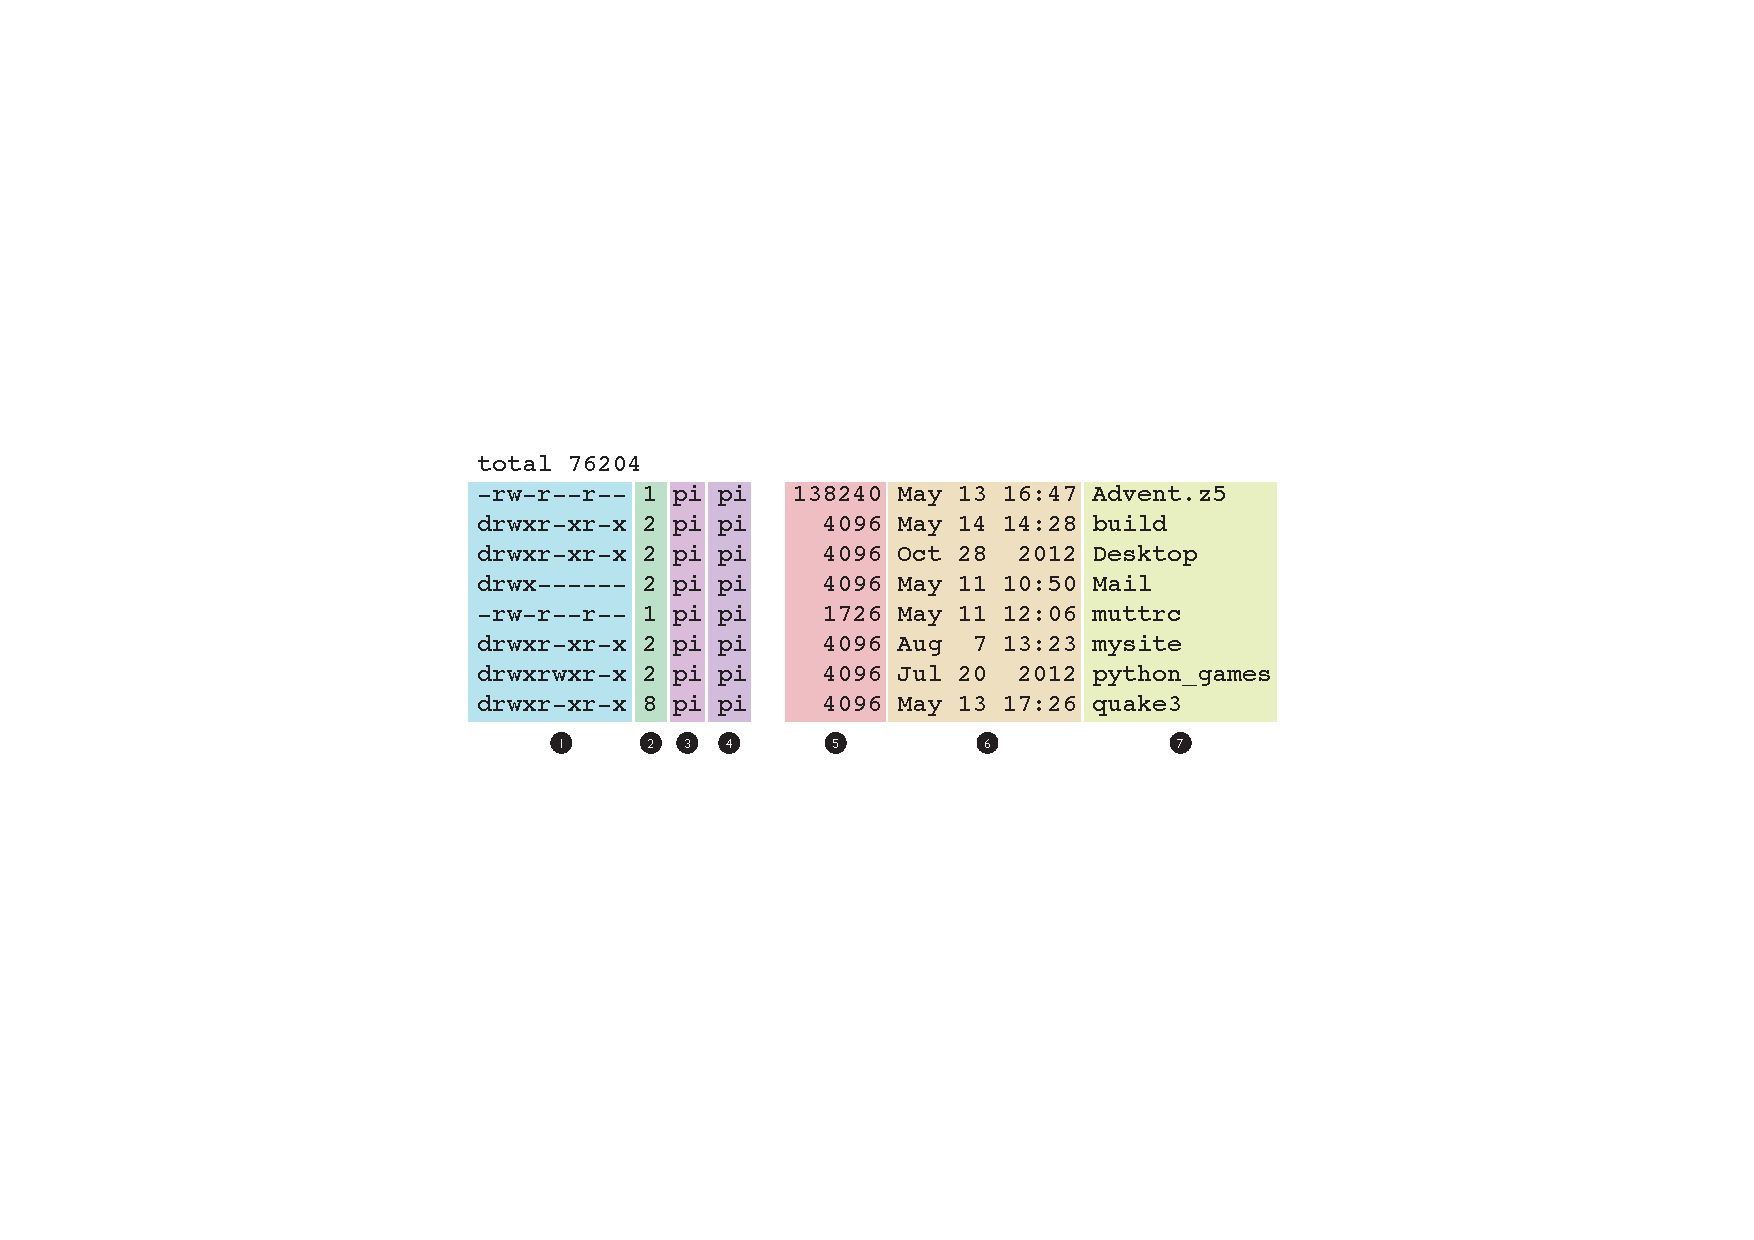
\includegraphics[width=14cm]{images/longformls}}
\caption{An example of the `long format' output from ls.}\label{figure:longformls}
\end{figure}

Working from right to left in Figure \ref{figure:longformls}, column \protect\circled{7} contains the filename, column \protect\circled{6} gives the date that the file was last modified (the exact format of the date will vary so as to always be `useful'; older files will have a year instead of an exact time, for example) and column \protect\circled{5} shows the size of the file in bytes. Columns \protect\circled{4} and \protect\circled{3} give the group and user to which the file belongs (often these will appear to be the same name); we'll come back to this in a moment. Column \protect\circled{2} shows the number of links associated with the file (ignore this for now), and finally column \protect\circled{1} gives a summary of the file's permissions, which we'll look at again shortly. 

In our example, the file's user (Column \protect\circled{3}) is not surprisingly `pi', which is the username under which you logged in. Run 

\begin{ttoutenv}
$ ls -l /
\end{ttoutenv}

(i.e. `long format list of the root directory), and you'll see that the files at the top of the filesystem are owned by a user called \ttout{root}. 

As well as being owned by a particular user, each file is associated with a \textit{group} (shown in column \protect\circled{4}, which in this case is a group called `pi' too; although both the user and the group are called pi here, they are different things). Every user is a member of one or more groups. The idea of a Unix group is quite straightforward: it's a mechanism to allow collections of users to share resources with one another in a controlled way, while stopping other unwanted users from being able to access those resources. For example, you might want to say ``Only I as this file's creator am allowed to modify or delete this file, but other members of my Tutorial Group can read the file's content, and the file is inaccessible to everybody else''. In Unix each file can have three different types of access permission: read, write and execute (run). These permissions can be set for three different categories of user: user (`owner'), group (a specific set of users) and `other' (which means `everyone else').

The file permissions shown in column \protect\circled{1} of Figure \ref{figure:longformls} consist of 10 `slots' as shown in more detail in Figure \ref{figure:fileperms}. The first slot indicates the type of the file, and appears as a \ttout{-} for a regular file or a \ttout{d} for a directory. The next three slots represent the \concept{user}'s  permissions and can consist of any combination of \ttout{r} for `readable', \ttout{w} for writable and \ttout{x} for executable. The next three slots show the read/write/execute permissions for members of the file's \concept{group}, and the last three slots show the same set of available permissions for \concept{other} (i.e. anyone else with access to the system). Execute permissions when applied to a directory mean that particular set of users can access the directory's contents.

\begin{figure}
\centerline{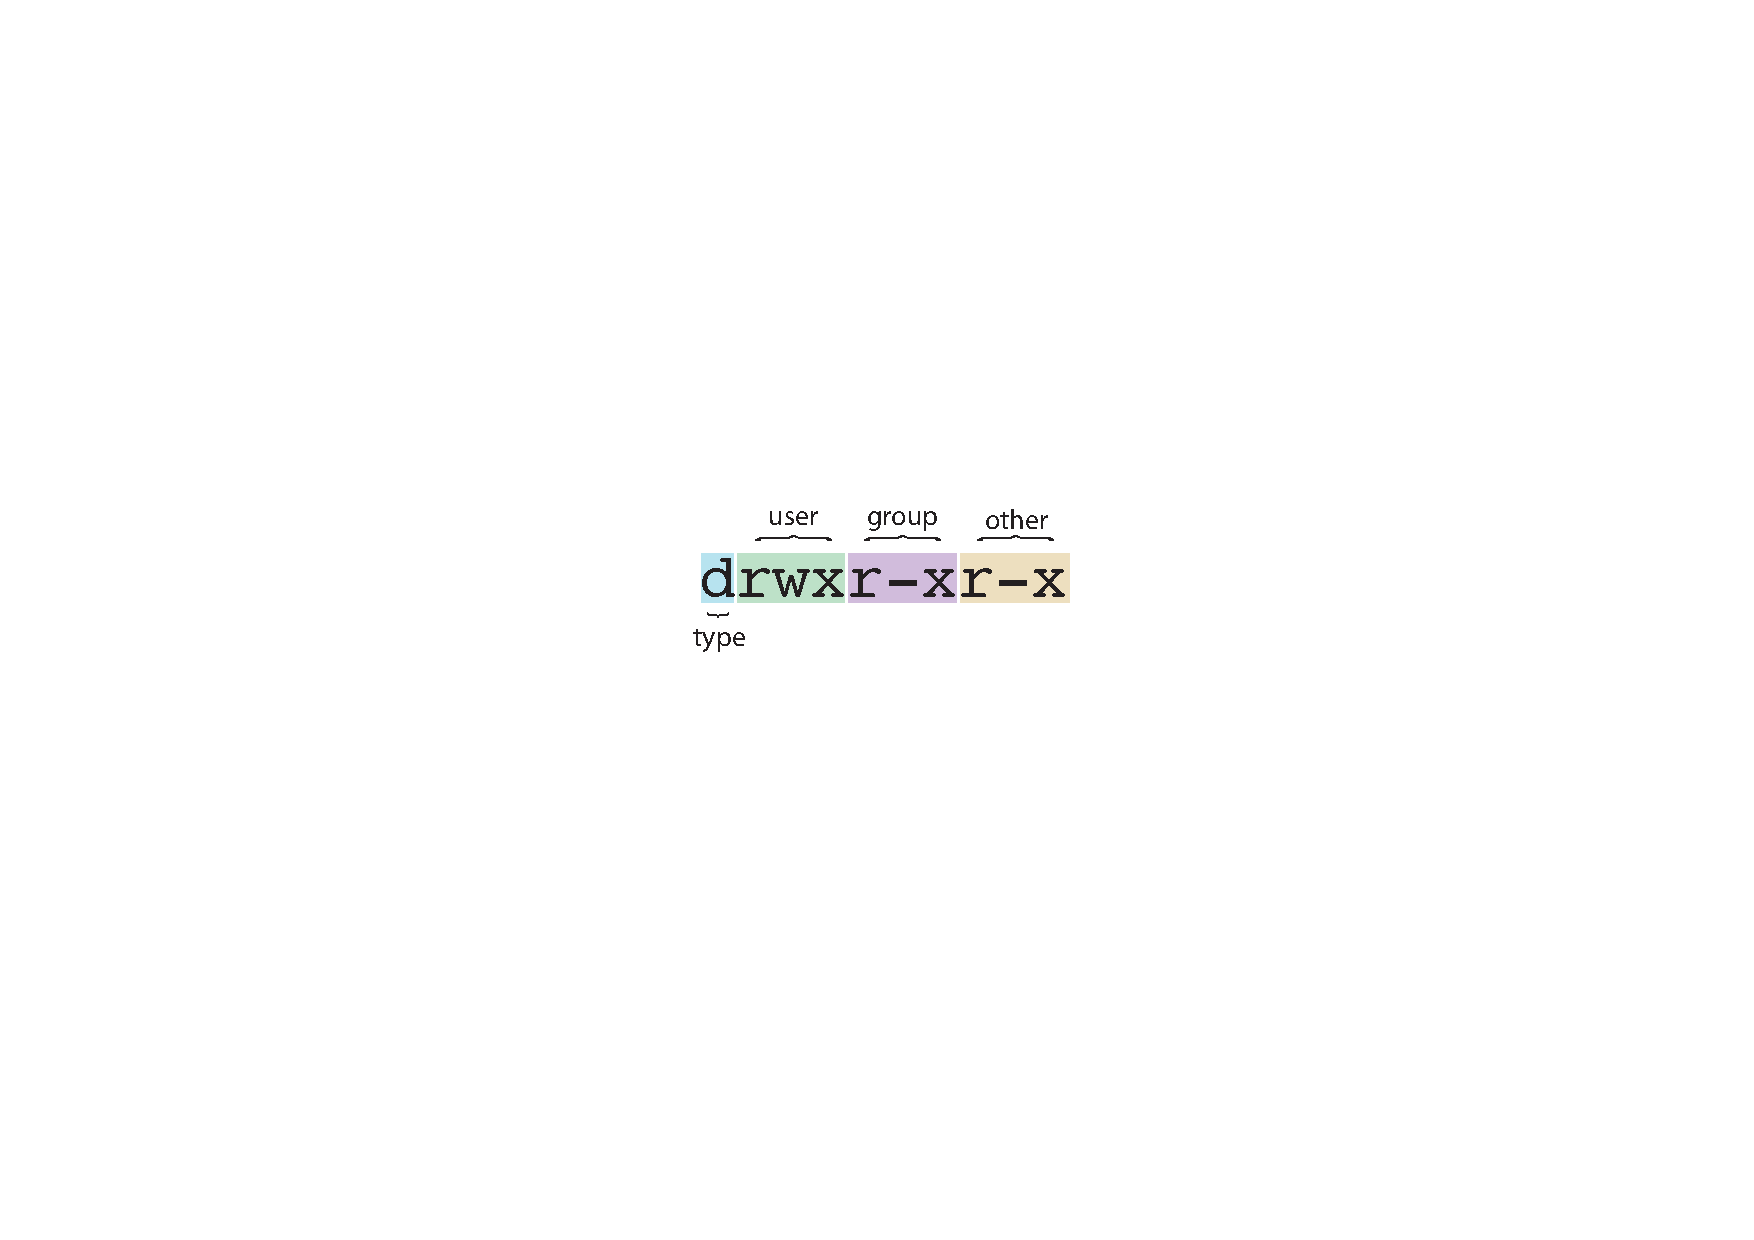
\includegraphics[width=7cm]{images/filepermissions}}
\caption{Unix file permissions as shown with \ttout{ls -l}. In this example shows the permissions for a directory that can be read from, written to and listed by its user (owner), but only read and accesed by group members or anyone else.}\label{figure:fileperms}
\end{figure}

We'll come back to file permissions in more detail shortly. In the meantime, let's look at the ownership model for processes. Type:

\begin{ttoutenv}
$ ps waux
\end{ttoutenv}
% $

to list any processes that are currently running (you'll probably need to widen the terminal window to see the output properly). The \cmnd{ps}{ps} command is unusual in that if used with no arguments, its output is largely uninformative. It's also unusual in that explaining what even the most basic arguments do and interact (i.e. the \ttout{waux} options in this case; note that there's no hyphen in front of the options here), is quite complex---so for now just treat this as a special recipe that does something useful. 

Look at the rightmost column of the output (which has the heading `COMMAND') and you should see a few familiar process names such as bash, \cmnd{startx}{startx}, and the \cmnd{ps}{ps} process itself in amongst many commands that will be unfamiliar to you at the moment. The rightmost column tells you who owns the processes, and you'll see that the majority of them are owned by you (or, rather by the user `pi'), and a small number of them are owned by the root user. Most of the processes that you're seeing have been started as part of the window manager system, or are in one way or another associated with X Windows; the rest are `housekeeping' processes the details of which we don't care about for now. 

If you think back to what you learned about the hierarchical relationship between processes in the first Pi lab, it should be starting to become clear how the `family tree' of processes when combined with the notion of users and resource ownership knit together nicely to give a secure multi-user system. When you first log in to a Unix machine, a single process is started on your user's behalf (in most cases this is a command shell). From that shell you can start other processes, which could be individual commands like \ttout{tar} or \ttout{ls}, or could be a whole window manager system such as Gnome or LXDE; in either case though, these inherit the properties of the parent shell in terms of being owned by the same user. Then, any processes that are started by the window manager also inherit the same user properties, and so forth. 

\subsection{Back to that webserver}

Anyway, let's get back to setting up the Apache web server. When you ran the python web server, that was a process owned by you, and because we didn't do anything special to protect it, if you closed the shell/terminal that was used to start it, it too would die. Generally speaking, you'd want a web server to continue running whether anyone was logged into the machine or not, so this isn't ideal. The other issue with starting a web server in this way is that because the process is owned by you, it has access to all your files---so if a malicious hacker was able to take control of the web server process, he or she would be able to read or even delete your work, which clearly isn't a good thing. 

So to set up a web server properly we need to

\begin{itemize}
\item make sure that it can continue to function after you've logged out, and
\item somehow make sure that it can only access a specific set of resources that represent the website, and not run riot around your filestore doing bad things. 
\end{itemize}

Let's first tackle the issue of a shared directory; this is quite easy to set up using Unix's group mechanism. 

By default, the Apache package that we're going to install shortly is set up to serve web pages from a directory called \fname{/var/www} and although you can change it in Apache's configuration files to be elsewhere, that's as good a place as any for what we need. 

Let's go ahead and install Apache using the command:

\begin{ttoutenv}
$ sudo apt-get install apache2
\end{ttoutenv}

It's a reasonably large package so may take a little while to install; just be patient. Once that's completed, take a look in \fname{/var} using \ttout{ls -l} and you should see a directory in there called \fname{www} which is owned by root.

Before we start serving any web pages, there are a few security issues that we need to take into account. In its simplest form, where you're just serving static web pages (i.e. HTML files), Apache is secure enough, but as soon as you start creating web sites where users can add and modify content on your server, you potentially open yourself up to malicious damage, so it's best to take some initial precautions. 

Take a look at the permissions for \fname{/var/www}, which was created when you installed the Apache package, and you will see that they are set to \ttout{drwxr-xr-x} which means `this is a directory that the owner can read, write and access the contents of, and which both group and other users can only read and access'. Notice too that there's a single file in that directory called \fname{index.html}, which is an `it works!' declaration that you can use to test that Apache is doing the right thing (and which we'll do shortly). The important thing here is that anybody or any process that is not running as the root user has only got \concept{read} and not \concept{write} access to the contents of the \fname{/var/www} directory structure---and this is exactly what we want. They can look, but not touch, and so can't break anything. 

But how do we get content into the \fname{/var/www} directory so that it can be served by Apache? We could simply use \fname{sudo} to give ourselves root privilege every time we need to modify a file, but that's a rather clumsy solution: we may not want other users on our machine to have root access at all, and in any case you really do want to keep sudo commands to a minimum so that you don't accidentally do something bad to your system. So let's create a new group that will represent users on the Pi that are allowed to put content into that directory. Use the command \cmnd{addgroup}{addgroup} to create a new group called \ttout{www-contrib} (for `web contributors'). The syntax is straightforward:

\begin{ttoutenv}
$ sudo addgroup www-contrib
\end{ttoutenv}

And you should see that a new group has been created with a Group Identifier (GID) probably set to 1001. 

Change the group ownership of \fname{/var/www} to be \ttout{www-contrib} using the command

\begin{ttoutenv}
$ chgrp -R www-contrib /var/www
\end{ttoutenv}

and check that this has changed using \ttout{ls -l}. Note that we're using the \ttout{-R} option to \cmnd{chgrp}{chgrp}, which means `apply this change not only to /var/www itself, but to all files and directories contained within it' (`R' here stands for \wikipedia{Recursion}{recursive}). Next we need to add the pi user to that group. Type

\begin{ttoutenv}
$ groups
\end{ttoutenv}

to see what groups your user is already a member of (you'll see things like \ttout{pi}, \ttout{adm}, \ttout{dialout}, \ttout{cdrom}, \ttout{sudo} and several others). Use the command 

\begin{ttoutenv}
$ sudo usermod -a -G www-contrib pi
\end{ttoutenv}

to add the Pi user to the www-contrib group. The \ttout{usermod} command can be used to modify lots of things about a user; here we are using with the combination of \ttout{-a} and \ttout{-G} to mean `append this group to the user's list of groups'. You'll need to log out and back in again to see this change take effect, so do that now and then run the \ttout{groups} command to confirm that pi is now indeed a member of group \ttout{www-contrib} as well as the other original groups. 

\begin{diversion}{About groups}
\label{diversion:aboutgroups}
Explain what the other groups are for
\end{diversion}

We now need to make the \fname{/var/www} folder \textit{writable} by members of our new group, so do that using the command

\begin{ttoutenv}
$ sudo chmod -R g+w /var/www
\end{ttoutenv}

which reads as `modify the permissions of the directory /var/www and any files/directories in it to add write access for members of its group'. 

Now if all has gone to plan, the user pi should be able to read and write to the directory \fname{/var/www}. Try this out by editing the content of the \fname{index.html} file that's in that directory (and which was created when you installed Apache) to say something different from the default text.

We're finally ready to start Apache. Use the Apache Control command

\begin{ttoutenv}
$ sudo apachectl start
\end{ttoutenv}

to initialise the server (you can use a similar command with `stop' to shut it down again), and then use \cmnd{ps}{ps waux} to confirm that you can see several processes with `apache' in the name now running. Note that although you started the server with \cmnd{sudo}{sudo} which runs things as root, that the owner of the apache processes is \fname{www-data}. The \ttout{apachectl} command has restricted apache to running as a regular, non-root user, and you should by now be able to work out why having a web server running as root would be a Bad Thing from a security point of view.

On the desktop machine use a web browser to see what content the Pi is now serving. The URL will be 

\begin{ttoutenv}
http://[IPADDRESSOFPI]
\end{ttoutenv}

and since we're now using a standard web server on a standard port, there's no need to add the :8000 port number as we did in Section \ref{section:headless}. 

You should see the `It works!' page appear, with whatever modification you made to it a moment ago.

Finally for this lab session, copy the content from your `aboutme' directory so that its served via Apache.  

\begin{note}
COPY OVER TO DESKTOP MACHINE, HALT THE PI and restore the desktop
\end{note}


%\chapter{Collaborative tools}

\renewcommand{\tilde}{\textasciitilde}
\newcommand{\moodle}{Moodle}
\newcommand{\Moodle}{Moodle}

\chapter[\Moodle\ Intro and command line skills]{Introduction to \Moodle\ and command line skills}

\minitoc

\notesurl{desktop2}


%\begin{note}
%  This is the fifth, two hour, lab.
%
%  Has change of position (?) of this lab made any difference to how we tell students about first tutorial?  Yes --fixed
%
%  Do we need some breakout boxes in this script?
%
%  \textbf{Steve's wish list}
%  \begin{itemize}
%  \item better navigation---more cd, pushd, popd, mkdir etc
%  \item 
%wildcards (use echo)
%\item 
%fortune | cowsay
%run fortune lots of times to make file
%\item 
%ls m * vs ls m*
%\item 
%revisit handy command line tricks 
%\item where do we introduce dot (as in ./splunge)
%
%  \end{itemize}
%
%
%\end{note}

This is the last of the introductory labs, and is designed to
introduce you to one of the virtual learning environments that's used
in the School, and to give you a chance to practise the command line
skills that you've learned already so that you're ready for when the
regular scheduled labs start. As always, don't rush through
the material, and if you get at all stuck please summon a demonstrator
for help.

\section{Getting started with \moodle}
\label{sec:introduction-moodle}

In the first half of session you'll be introduced to the \moodle\ Virtual Learning Environment (VLE). \moodle\ is an \wikipedia{Open_source}{Open Source} platform designed to support face-to-face teaching by providing an online place to upload resources for course units. It also provides useful tools such as discussion forums and quizzes. We use \moodle\ for several of our course units, which typically have a single `course unit site' within our \moodle\ environment.

%Why is Moodle being used for COMP10120
\moodle\ has several features which make it well suited to supporting this course-unit. These include:
\begin{itemize}
\item It's one useful way of communicating with your tutor and members of your tutor group.
\item It allows us to give each group a wiki which you'll use to collaboratively document your project work.
\item It provides a structure to help organise activities you should be doing on a week-by-week basis.
\end{itemize}

Log in to \moodle\ by pointing your web browser at:
\\

\url{http://moodle.cs.man.ac.uk}
\\

and using your University username and password. 

After successfully logging into \moodle\ for the first time, you'll be presented with a form to complete the details of your \moodle\ profile. Add your first and last names; your email address; the city/town where you live (for most people this will be Manchester); and add a short description of yourself. Select the `Update profile' button to complete your \moodle\ registration. Assuming that worked okay, the next page to appear will be the \moodle\ home page (see  Figure~\ref{figure:moodle-home})

\begin{figure}
\centerline{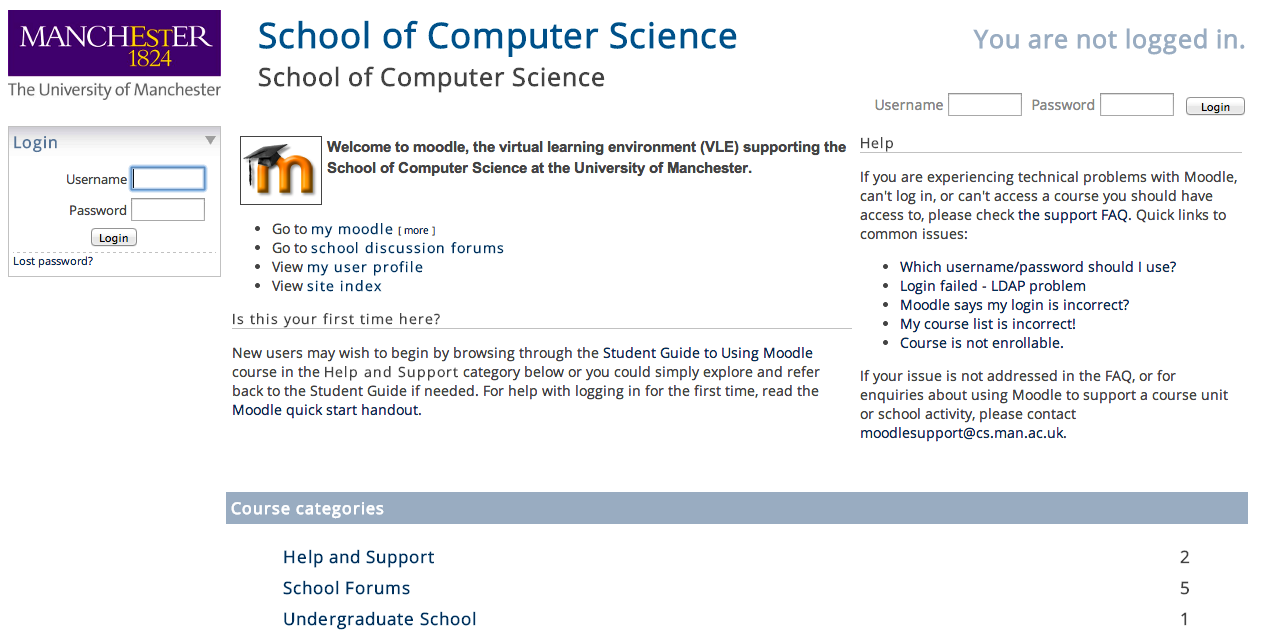
\includegraphics[width=15cm]{images/moodle-home}}
\caption{Moodle Home Page}\label{figure:moodle-home}
\end{figure}

Take a few minutes to browse though the \emph{Getting started with \Moodle} guide which is deliberately located outside the \moodle\ environment so that you can get at it in case you're having problems with \moodle\ itself. You can find it at: \urlnop{octette.cs.man.ac.uk/moodleintro} (see Figure~\ref{figure:moodle-start}).

\begin{figure}
\centerline{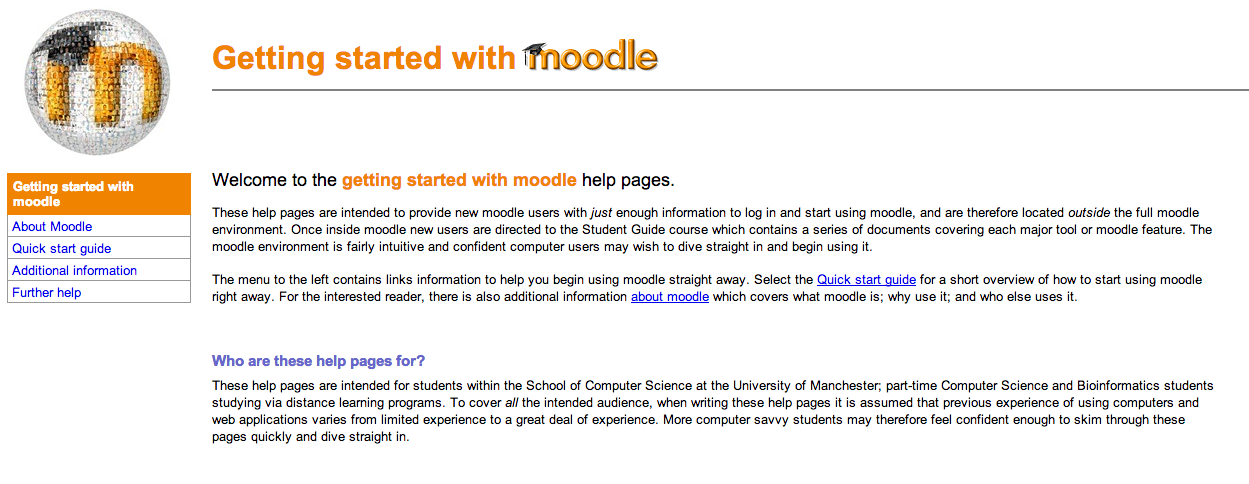
\includegraphics[width=15cm]{images/start-moodle-page}}
\caption{Getting started with Moodle}\label{figure:moodle-start}
\end{figure}

\subsubsection*{Brief overview of the \moodle\ home page}
\label{sec:brief-overv-moodle}


The \moodle\ home page lists several categories in which \moodle\ course unit sites are organised (make sure you scroll down to see them all). \moodle\ course unit sites exist for many, but not all, course units within your degree programme.

You can find links to sites by either locating the link in the appropriate category, for example look in \emph{Undergraduate School/First Year} for COMP10120; or you can enter \emph{COMP10120} into the \emph{Search courses} field at the bottom of the course list and select the course unit title from the search result(s).

Other things to look out for on the front page include the link to your \moodle\ user profile and the link to the \emph{my moodle} feature. We'll come back to these later on.


%Your turn


Make sure you can find the COMP10120 course unit site and are able to access it. To get back to the \emph{\moodle\ home page} you should click on the \moodle\ link in the navigation bar underneath the course unit title at the top of the page. This is always the first element in the link trail. If you navigate further into the course unit site, to return to the \emph{course unit site front page} just click on the COMP10120 link in the navigation bar. This is always the second element in the link trail.

Now locate the course titled \emph{Student Guide to Using Moodle} (in the category \emph{Help and Support}). Have a browse through what help material is provided here. You may wish to revisit this site to learn how to use one of the \moodle\ activities or understand one of \Moodle's features.

\subsection{The COMP10120 course unit site}
\label{sec:comp10120-course-uni}


If you haven't already, navigate to the COMP10120 site and start to look at how the site is structured and what tools have been provided (see Figure~\ref{figure:101-moodle-page}).
Here are some things you should note about the structure of the site:

\begin{figure}
\centerline{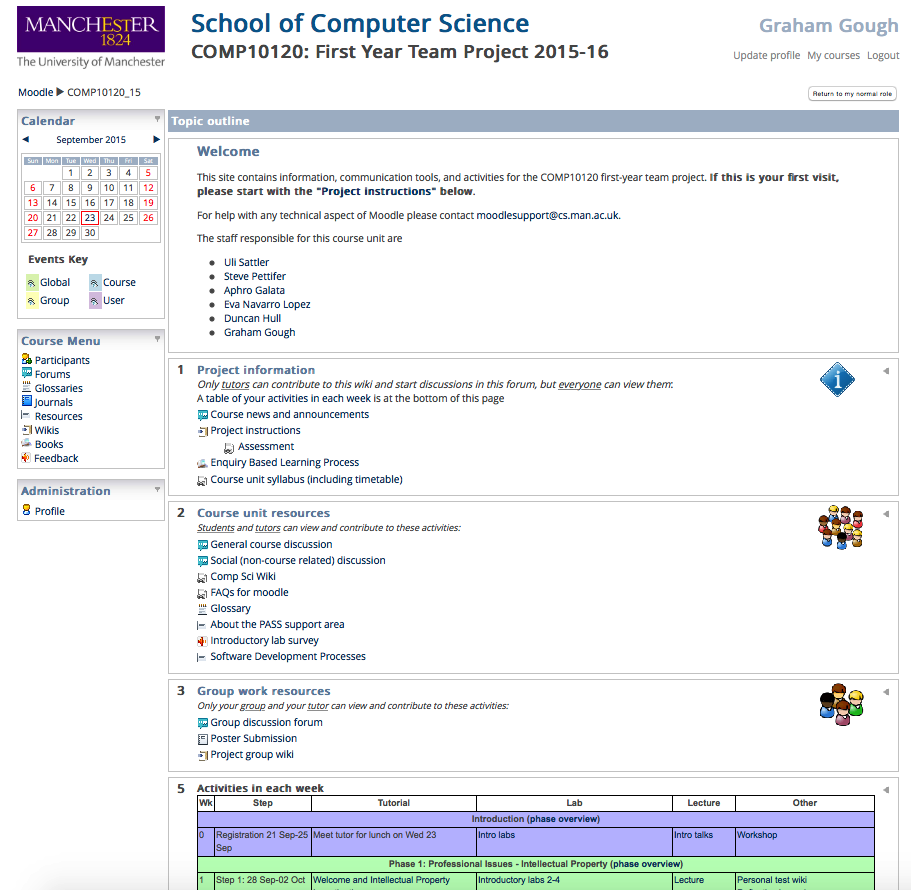
\includegraphics[width=15cm]{images/101-moodle-page}}
\caption{COMP10120 Moodle Home Page}\label{figure:101-moodle-page}
\end{figure}


\begin{itemize}
\item 
All instructions for the course unit are located in the \emph{Project information} area towards the top of the site. Take a look at each of the links in this area. In particular, familiarise yourself with the front page of the \emph{Project instructions} and read at least the \emph{Introduction to the tasks and activities} (and then click through to the \emph{Phases and Tutorials} page to get an idea of the course unit structure).

\item Back on the course unit site, the next section is called \emph{Course unit resources}. If you have a query about the course unit, please use link to the \emph{General Course Discussion Forum}.

\item The next section is called \emph{Group work resources}. This is your tutor group's area and should be used to communicate with members of your team (by using the forum) and to document your work (in the wiki).

\item Finally, the bottom of the course unit site has a table of all your activities for this course-unit. The different phases are colour-coded to help you spot the one you want. The row for each week contains links to information about what you should be doing in that week and tools/resources applicable to the week. (Don't forget to read the \emph{phase overview} first.)

  The \emph{Other}  column includes resources for your personal use, that you are expected to complete over the course of the year. In particular you should note the \emph{reflective journals} for each week of the first semester. You are expected to reflect on the questions detailed inside the journal each week.
\end{itemize}

% The remaining instructions for this lab session can be found
% directly within \moodle\ itself. Click on \emph{Introduction to \Moodle} % in the \emph{Lab} column for \emph{Step 1} in the green (\emph{Phase 1}  section.

\subsection{Lab deliverables}
\label{sec:lab-deliverables}

By the end of this section of the lab session, ensure you have completed the following tasks.

\begin{itemize}
\item 
Posted a welcoming message to your tutor group (see Using forums below).

\item Create your set of practice wiki pages (see Using wikis below).

\item Completed the Individual Learning Profile questionnaire
\end{itemize}

%There are also a number of optional tasks you should aim to complete if you have time during the lab.

\subsection{Using forums}
\label{sec:using-forums}


Most of you will have used discussion forums in some way or another, whether on your favourite social networking site or on some other website. \Moodle's forums aren't too different to any other, however, you should note a few things:

Most forums are configured so that copies of each posting will be emailed to other course unit members. In a group forum, copies are only emailed to other group members; in a course forum copies are emailed to everyone.

In most cases you will have the option to remove your subscription to such emails. Please don't do this, at least not at the moment.

In your user profile you have the option to receive \moodle\ emails as a single daily digest rather than as multiple emails each day; if you're finding you're getting a lot of email from \moodle\ this might be a sensible option to select (but keep it mind that you'll lose some of the immediacy of receiving individual emails). 

You might not be able to post messages in all forums. Some forums (e.g. course announcement forums) will only allow tutors to start new topics of discussion, but will allow students to reply to those topics once started.

%Your turn
Visit your Group discussion forum on the COMP10120 site and click on \emph{Add a new discussion topic}  to begin a new discussion thread. Write a short forum posting to introduce you to your other group members and your tutor. Let them know where you are from, tell them a little bit about yourself.

Note that your discussion posting won't be emailed to the other members of your group until about 30 minutes after you submit the posting. This is to allow time for you to edit it in case you spot a mistake.

If you want to find out more about using discussion forums, look through the \emph{How to use the forums}  help book in the \emph{Student Guide to Using \Moodle} course. There is also a help book called \emph{Using \moodle's HTML editor} which you may also find useful.

\subsection{Using wikis}
\label{sec:using-wikis}


You have almost certainly come across wikis before, and will no doubt have looked things up in \wikipedia{Wikipedia}{Wikipedia}, the world's biggest wiki, many times. Unlike many other online collaboration systems which constrain users in various ways by pre-determining the type of content that can be created (for example sites like Instagram and Flickr are designed for sharing photographs, where as Soundcloud is for sharing audio), and also categorising users as having different types of access (e.g. administrators, moderators, regular users and so forth), the technology behind wikis typically takes a very liberal approach to both users and content. They generally allow any user to make any kind of change to any kind of content, and rely on \textit{social} conventions established by the community to keep things sane. In particular, every edit, deletion and addition to the wiki is stored, providing a complete history of wiki changes. Old versions of pages and be retrieved and compared to new versions of pages. Wikis are typically edited using a simple mark-up syntax where the focus is on content rather than fancy presentation.


As well as creating sites like Wikipedia, wikis are frequently used by software development teams to document their project. The ability to look back to previous versions of documents and the for multiple authors to collaborate on producing the documentation without having to worry too much about `process' is particularly useful in such environments.

During COMP10120 you'll required to document many aspects of your work using a group wiki provided by \Moodle. \Moodle's wiki isn't as powerful as others you may have come across as it is primarily tailored towards teaching, but it does allow you to use \Moodle's standard in-line HTML editor to help you with formatting.

%Your turn
In the bottom \emph{Resources for individual use} section of the COMP10120 site you will find a link to a wiki called \emph{Personal test wiki} which is private for you and you only. It is provided to allow you to practise how to use \moodle\ wiki syntax before you start using your shared group wiki. If you have used a wiki before then you may find \Moodle's wiki syntax is slightly different to that which you are used to.

For this short exercise you will need to read through some of the help documentation hosted inside \moodle. In a new window or tab navigate to \urlnop{moodle.cs.man.ac.uk} again and enter the \emph{Welcome to the Student Guide to Using \Moodle} course in the \moodle\ \emph{Help and Support}  category (you may be asked to 'enrol' on this course, just select 'Yes'). Scroll down to the section about Wikis and select the \emph{How to use the wiki tool} book.

The aim of this short exercise is to create a simple wiki page with two or three wiki links to other pages; incorporate an image; and attach and link to a binary (non-image) file. It is important that you follow this mini-tutorial through to the end as it will ensure you know how to do all the basic tasks needed to help build your own group wiki during the project.

For the purposes of this mini-tutorial you are asked to create a small wiki about yourself.

Start by opening your Personal test wiki. You will be presented with the \moodle\ editor which won't contain any content yet. Enter a title for the page, something like \emph{About Me} will do.

Select the \emph{Save} button. You should now see the first page of your wiki with the content you just added. Now select the \emph{Edit} tab so that you can add more content.

Create a short bullet list containing the items \emph{My hobbies},  \emph{My music}  and \emph{My files}  Save the page again and check the results, then select the Edit tab again. Now turn the three items into wiki links. To do this, just put a single set of square brackets around each of the terms, like this: \emph{[My hobbies]}  \emph{[My music]}  \emph{[My files]}  Save the page again and look at what just happened. If everything worked correctly each term enclosed in square brackets should now look like this: \textbf{term}? (emboldened text followed by a hyperlinked question mark).

Select the question mark symbol on the \emph{My hobbies} term. Note this opens up a new wiki page called \emph{My hobbies} for you to populate with content. Add some text to describe a few things about what you like to do with your time and then select Save.

This is the basic process by which you build up a wiki into a series of linked pages. Note that at the bottom of the page you just created is a list of \emph{Referring links}  This means \emph{a list of pages that link to this one}  Select the link back to the front page.

In the Student Guide to Using \moodle\ course look at the help book on wikis and read the chapter titled \emph{Unique names for pages}  in particular instructions on how to make the link text different from the linked page name. Now go back and change your first wiki page so that the link to the page \emph{My hobbies} contains the link text \emph{My interests} (but still points to My hobbies). Your list should now contain the items \emph{My interests},  \emph{My music}  and \emph{My files} 

Now go back and select the question mark link for the \emph{My music} link and add some content to this page too. You could write about music you love (or music you hate!).

In the last part of this mini-tutorial, you will need to add a small picture to your wiki and a small file. First we need some files to play with. If you have a small picture that you took yourself, great, you own the copyright on it. Create a small text file using any text editor containing any text you like. If you don't have a picture to use and can not source a copyright free image, you will find a link to an example image in the summary text box of the wiki above the first page. There is also a link to a sample text file there too.

In the Student Guide to Using \moodle\ course look at the help book on wikis and read the chapters titled \emph{Attaching binary files} and \emph{Linking to attached files}  From your wiki's front page select the question mark link for the \emph{My files} link to create its page content. Attach your text file to the page from the wiki's Attachments tab as described in the \emph{Attaching binary files} chapter of the help book. Then return to the edit tab and add the following text:

\emph{Wikis allow users to attach files, such as this one here}  

Turn the word \emph{here} into a link to the text file you just uploaded following the instructions in the \emph{Linking to attached files} chapter of the help book.

Carefully read the chapter of the help book titled \emph{Incorporating images}  Now add the following text and add the image you grabbed earlier below the text.

\emph{Wikis also allow users to incorporate images such as this one.} 

Experiment with changing the alignment of the image as described in the help book.

Finally, browse through the remaining documentation in the Wiki help book so that you have an overview of what other information is there and can refer back to it in the future if needed. If you have any questions about how to use the wiki tool, post a message to the General course unit discussion forum.

\subsection{Individual Learning Profile questionnaire}
\label{sec:indiv-learn-prof}

Before the end of the lab session make sure you complete the \emph{Individual Learning Profile questionnaire}. You will find it in the \emph{Resources for your individual use} section at the bottom of the \moodle\ course unit site. This activity is to help you to reflect so that you can understand your own basic skills and abilities required for your academic life. It may also be looked at by your personal tutor so the School can be better placed to address your particular needs during your time in the School of Computer Science. This information will only be visible to you, to your tutor and to the course unit organisers.

\subsubsection*{Writing your journal}
\label{sec:writing-your-journal}


One of the aims of this course unit is to encourage you to develop the habit of thinking about the way you are learning and working, and trying to identify ways in which these could be improved. The process of reflection is key to this, but is not something that comes naturally to many of us. In most week slots of the course unit site you will find an instance of the Journal activity. The summary text of each journal contains prompts to aid your reflection that week. The journal is very simple \moodle\ tool which provides you with an editable text area supported by \moodle\ HTML editor. Selecting the \emph{Start or edit my journal entry} button opens your journal. Any entries you put into your journal will be completely private to you and your personal course unit tutor. A limited number of the course unit organisers have access to all students journals, but will respect your privacy and will not be looking at them.

At some time towards the end of this week, start your journal entry for the current week and post your answers the prompts provided.

\subsection{What else is on \moodle?}
\label{sec:what-else-moodle}


As well as course unit sites for many of your course units, there are also a number of open areas within \moodle. Within the \emph{Support Forums} category you will find a number of sites where you can seek help about specific areas within computer science, e.g. the C / C++? Programmer's Forum. The \emph{Student / Staff Groups} category includes a site where you can post up questions or topics of discussion for the Staff Student Consultative Committee. All these open courses are indicated by the guest user icon (a small person icon or a side-on face depending on your chosen \moodle\ theme). Have an explore and see what is there. More open site are likely to be added over the year.

% \subsection*{Playing and personalising}
% \label{sec:play-pers}


% If you have time left in the lab session, spend some time personalising your \moodle\ account. Things you could do include:

% Uploading a small photo or image to represent yourself to your \moodle\ profile.

% %Personalising your my \moodle\ area.

% Take a closer look at the advanced options in your \moodle\ profile and investigate what they do (read up about this in the \moodle\ help course books first).


% % Look ahead on the COMP10120 site to get a feel for what you will be doing over the coming year.

\subsection{Another VLE: Blackboard}
\label{sec:blackboard}

You won't be using it for this course-unit, but for your other course-units you may be using a different Virtual Learning Environment: \textsf{Blackboard}. The usual way to access \textsf{Blackboard} is via the \href{https://my.manchester.ac.uk}{\emph{My Manchester}} page at \urlnop{my.manchester.ac.uk}, and then use the \emph{'My Blackboard'} tab. There is also a plentiful supply of information about how to use Blackboard available online. 

That's all we want to say about Moodle and VLEs. The second part of this lab is about using the command line in Linux.


\section{Reinforcing your command line skills}
\newcommand{\cmdname}[1]{\cmnd{#1}{#1}}
\newcommand{\ilinput}[1]{\ttout{#1}}
% \newcommand{\crsname}{COMP10120}
% \newcommand{\Dcrsname}{\fname{/opt/info/courses/COMP10120}}
% \newcommand{\crsnamelc}{comp10120}
\newcommand{\crsname}{INTRO}
\newcommand{\Dcrsname}{\fname{/opt/info/courses/INTRO}}
\newcommand{\crsnamelc}{intro}
\newcommand{\return}{\relax}

This section is designed to help you practise your command line skills in preparation  for next week's start of regular lab activities. You've already used most of these commands in previous labs, but please don't rush through this section since we'll be explaining their behaviour in a bit more detail, and introducing you to some of the extra options they provide, as well as some of the pitfalls that lie in wait for the over-zealous command line user.  

You've probably figured this out already, but it's worth making explicit here: for Unix commands, it's usually the case that no news is good news. So when you run a program from the shell, if you get no response other than your command-prompt back, that almost always means that the command has done what you asked it to (whether you asked it to do what you \textit{wanted} it to do is, of course, an entirely different matter!) Generally speaking, for most simple Unix commands, you can assume that the absence of an error message means that something has worked. And of course, if you get an error or warning message back from a command, it is crucially important that you read it, understand it, and act on it, rather than just ploughing on regardless. If you ignore errors and warnings, bad things happen. This is true in the Unix command world, and probably isn't a bad philosophy for life in general either.

Anyway, back to the exercise and some practice of manipulating files and directories. In previous labs you've already encountered three directories of particular interest:

\begin{itemize}
\item The \concept{root directory} (\ttout{/}) is the top level of the
\concept{file system}.
%??? file system or filesystem ???

\item Your \concept{current working directory} which is the one your are `in'
at the moment (and is shown by the output from \cmdname{pwd}). This can also
be referenced using a single dot (\ttout{.}), as in when starting up Quake Arena using 
\ttout{./ioquake3.arm} in your first Pi lab. 

\item Your \concept{home directory} (\ttout{\tilde}) which is the top level of
your own filestore and where \cmdname{cd} (\concept{change directory}) with no
arguments will take you.  The value of this is also available as
\ttout{\$HOME}, so the following all have the same effect:

\begin{ttoutenv}
\$  cd
\end{ttoutenv}
or
\begin{ttoutenv}
\$  cd ~ 
\end{ttoutenv}
or
\begin{ttoutenv}
\$  cd \$HOME
\end{ttoutenv}

And no matter what is your current working directory, you can list the files
in your home directory with either of these commands.

\begin{ttoutenv}
\$  ls ~
\end{ttoutenv}
or
\begin{ttoutenv}
\$  ls \$HOME 
\end{ttoutenv}

\end{itemize}

You should recall the difference between an \concept{absolute path} (one
that starts with \ttout{/}) and a \concept{relative path} (one that does not
start with \ttout{/} but is instead `found' relatively) by starting in the
current working directory. You've met the `double dot' notation
(\ttout{..}) to mean `go up one level', as in \ttout{ls ..} or perhaps more
often \ttout{cd ..}, or even \ttout{cd ../x/y} and so forth.

Speaking of \cmdname{ls}, you will from time to time need to use its
\ttout{-a} switch argument to ask it to show `hidden' files beginning with a dot,
and/or \ttout{-l} to make it show details about the files it lists.

\subsection{Creating a directory structure}

Use the \cmdname{mkdir} (\concept{make directory}) command
to create some directories. Type:

\begin{ttoutenv}
\$  cd
\$  mkdir \crsname\return
\end{ttoutenv}
%
and check that this directory has indeed appeared using \cmdname{ls}.

It's important that directories we ask you to make for your work have
exactly the names we specify: Unix will let you use any names you
like, but so that demonstrators and staff know where to look for stuff when you get marked, and so that the system you'll be using to submit your work knows what you're submitting, it's very important that you follow these conventions for your lab work. Any files and directories you create for your own purposes outside of lab work can of course be named and organised however you like.

If you made a mistake, e.g. \fname{\crsnamelc} instead of \fname{\crsname},
you can remove the directory \textit{while it is still empty} with the
\cmdname{rmdir} command: e.g.
%
\begin{ttoutenv}
\$  rmdir \crsnamelc\return
\end{ttoutenv}
%
And then try to make it correctly.

%The \cmdname{cd} (\concept{change directory}) command allows you to move around
%the tree by changing your current working directory. Type
%%
%\begin{ttoutenv}
%\$  cd \crsname\return
%\end{ttoutenv}
%%
%to make \crsname{} your working directory. Check that you have changed
%current directory using \cmnd{pwd}{pwd}.
  
Now go into your \ttout{INTRO} directory and let's make some make directories for four imaginary \crsname{} exercises.

\begin{ttoutenv}
\$  mkdir ex1 ex2 ex3 ex4\return
\end{ttoutenv}
%  mkdir ex1 ex2 ex3 ex4 \return
%
%Recall that the \cmdname{cd} command on its own takes you back to your home
%directory, wherever you may be when you invoke it.  Try this out by
%typing
%
%\begin{ttoutenv}
%\$  cd \return
%\end{ttoutenv}
%
%Check that you are now in your home directory.
Now return to your home directory.

Your directory structure should now look something like this:
%\begin{firstonly}
     \begin{center}
       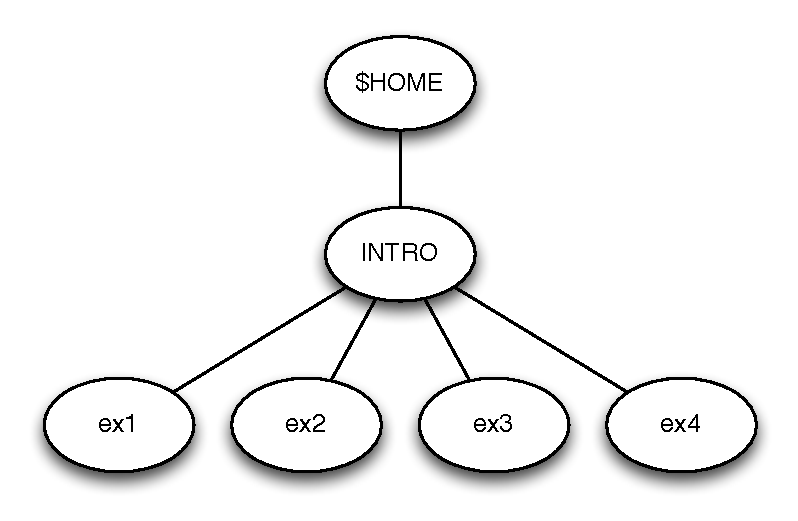
\includegraphics[width=0.6\textwidth]{images/intro-dir-structure}
     \end{center}
%\end{firstonly}

The easiest way to check this is to use 
\cmdname{ls} from your home directory with the \ttout{-R} flag. This shows the whole tree
below your current working directory (as with other commands we've encountered before such as \cmdname{chmod}, here the \ttout{-R} is short for
\wikipedia{Recursion}{recursively}---if you've not looked up what this means yet, now is a good time to do that).

\begin{ttoutenv}
\$ ls -R 
\end{ttoutenv}
%

Next make a directory in your home directory for the
\courseunit{COMP16121} course unit with sub-directories for each of the 10
exercises associated with that course (these aren't imaginary exercises, you'll be starting on them next week). You \emph{must} use the same
convention as above: capital \texttt{COMP16121} and lower case \texttt{ex1} and so on.

You must get your directory structure right before continuing---be extremely careful that you get this right.

%ask a member of the lab staff to check it at this point.

%\begin{note}
%Do we really want them all to ask a demonstrator?
%\end{note}

%Every directory is created with two files already there, called `.'
%and `..'. Of course, you don't see them when you run \cmdname{ls}
%because they start with a dot! Now run the command which will enable
%you to see them in your current directory.
%
%`.' is a reference to the directory itself, and `..'is a reference
%to the directory above it in the tree. This may seem rather bizarre at
%first, but they are in fact extremely useful.  `..', for example,
%enables you to specify a \emph{relative} pathname \emph{up} the tree.

Try the following sequence of \texttt{cd}s, checking where you are by running \cmdname{pwd} after each one, and make sure you understand what is going on: if you're at all unsure about what has happened, please grab a demonstrator to get an explanation---it really will save you a lot of hassle in the long run. 

\begin{ttoutenv}
  cd \return 
  cd \coursename/ex1 \return 
  cd .. \return 
  cd ex2 \return 
  cd ../ex1 \return 
  cd ../../\coursename/ex2 \return 
  cd ../.. \return
\end{ttoutenv}
%

\subsection{Copying, moving, and removing files}

This subsection re-introduces three commands used for copying, moving and
removing files. We'll first describe each command and then you'll get an opportunity  to practise using them.

\subsubsection{Copying files: cp}

\noindent The \cmdname{cp} (copy) command has two forms.

% \begin{note}
%   fix $<$file$>$ [file] notation
% \end{note}

The first general form is
\begin{ttoutenv}
\$  cp [FILENAME] [FILENAME] \return
\end{ttoutenv}

For example

\begin{ttoutenv}
\$  cp file1 file2 \return
\end{ttoutenv}
%
makes a copy of the file \fname{file1} and calls it \fname{file2}.  If
a file called file2 already exists, \emph{the existing \fname{file2} will be  overwritten
with a copy of \fname{file1} and lost without warning}.

The second form is slightly different:
\begin{ttoutenv}
\$  cp [FILENAME(S)] [DIRECTORYNAME]
\end{ttoutenv}
%
For example

\begin{ttoutenv}
\$  cp file1 file2 file3 dirname \return
\end{ttoutenv}

This copies the files \fname{file1}, \fname{file2}, \fname{file3} into
the directory \fname{dirname}, again overwriting any files already
there with the same names.

\subsubsection{Removing/deleting files: rm}

The command \cmdname{rm} (remove) is used to delete files.
\begin{ttoutenv}
\$  rm [FILENAME(S)]
\end{ttoutenv}
%
throws away the specified files. Always take great care when using \cmdname{rm}: unlike putting things in the `trash' or `recycle bin' in a desktop environment, the effects of \cmdname{rm} are \textit{not reversible}, and you don't get any warning before files are \textit{deleted forever}. 


\subsubsection{Moving / renaming files: mv}

The \cmdname{mv} (move) command is similar to \cmdname{cp}, but it just moves
the files rather than makes copies. Again we have the two forms
\begin{ttoutenv}
\$  mv [FILENAME] [FILENAME] \return
\end{ttoutenv}
and
\begin{ttoutenv}
\$  mv [FILENAME(S)] [DIRECTORYNAME] \return
\end{ttoutenv}

The effect is like a copying followed by removing the sources of the copy,
except it is more efficient than that (most of the time).
For example
\begin{ttoutenv}
\$  mv file1 file2 \return
\end{ttoutenv}
is like doing
\begin{ttoutenv}
\$  cp file1 file2 \return
\$  rm file1
\end{ttoutenv}
and
\begin{ttoutenv}
\$  mv file1 file2 file3 dirname \return
\end{ttoutenv}
is like doing
\begin{ttoutenv}
\$  cp file1 file2 file3 dirname \return
\$  rm file1 file2 file3
\end{ttoutenv}


\begin{diversion}{Taking out the trash}
You now know enough about the behaviour of the filesystem to know what's actually going on when you put files in the `recycle bin' or `trash can' in a desktop environment such as you get with OS X, Windows or Gnome. When you `move to trash' in these environments, you're not deleting the file but instead using an equivalent of the \cmdname{mv} command to move the file from its current location into a special directory that represents the trash can. When you tell the graphical environment to `empty trash', you're actually invoking something equivalent to \cmdname{rm}, which actually does delete the file from the filesystem.
\end{diversion}

%\begin{note}
%
%This seems a bit of an odd thing to put in a section about mv. Do we still want to say this?
%
%Before continuing, answer this question and check your answer with a
%member of staff: how do you \emph{rename} a file in Unix? Don't guess---you
%know the answer, unless you have already forgotten from previous labs and you are now going too fast.
%\end{note}


\subsection{Practice makes perfect}
Now for some practice. Go to your home directory by typing:
%
\begin{ttoutenv}
\$  cd \return
\end{ttoutenv}
%
and copy the file called \fname{fortunes} in the \fname{/usr/share/games/fortune}
directory to your current working directory, by typing

\begin{ttoutenv}
\$  cp /usr/share/games/fortune/fortunes \textbf{.}  \return
\end{ttoutenv}
%
Note that the dot (meaning, of course, your current directory) is
essential.  If you now do an \cmdname{ls}, you should see that the
file called \fname{fortunes} has appeared in your directory:

\begin{ttoutenv}
\$  ls \return
\end{ttoutenv}

If no file called \fname{fortunes} has appeared, the following will
probably provide an explanation. If it did appear, read this anyway, just to
check that you understand what you did right.

The \cmdname{cp} command needs at least \emph{two} arguments. In this case, the file
you are copying is \fname{/usr/share/games/fortunes}, and the directory
you are copying it to is `.' (that is, your current working
directory; remember every directory has a reference to itself within
it, called `.') If you missed out the dot, or mis-spelt
\fname{/usr/share/games/fortunes}, or missed out one of the spaces, it
won't have worked. In particular, you may well have got an error message like:
%
%  Usage: cp [-ip] f1 f2; or: cp [-irp] f1 ... fn d2
\begin{ttoutenv}
  cp: missing destination file
  Try `cp --help' for more information.
\end{ttoutenv}
%
or
\begin{ttoutenv}
  cp: /usr/share/games/fortunes/frotunes: No such file or directory
\end{ttoutenv}
%
If you get the first message, it means you used the command with the
wrong number of arguments, and nothing will have happened.
The other is an example of what you might see if you mistype the first
argument. If you do get an error message you need to give the command again,
correctly, to copy the fortunes file across.

\begin{linux}{fortune}
  \label{breakbox:fortune}
  At the moment we're just going to be using the fortunes file as something to copy and move around, so its contents are not important, but it's one of the source files used by the unix \wikipedia{Fortune_(Unix)}{fortune} command, which we will be playing with later.

  \wikipedia{Fortune_(Unix)}{fortune} is a simple program that displays a random message from a database of (supposedly) humorous quotations, such as those that can be found in the US in \wikipedia{Fortune_Cookies}{fortune cookies} (hence the name). It also contains jokes (of a sort!) and bits of poetry.

\end{linux}

You should now have a copy of the file in your home directory.
You'll have to get into the habit of \emph{not} having all your files
in your home directory, otherwise you will quickly have an enormous list
of stuff that will take you ages to find anything in. The use of subdirectories
provides a solution to this problem, which is why you created some
earlier. Moving this file to the `correct' place gives you a chance
to practise the \cmdname{mv} command.

Move the file \fname{fortunes} to your \fname{\crsname/ex4} directory.

% Notice that \fname{\crsname} is \emph{your\/} \crsname{} directory, while
% \fname{\Dcrsname} is (an abbreviation for) \emph{our\/} \crsname{}
% directory, from which you can read things but cannot write to.

Now go to your \fname{\crsname/ex4} directory and check that the file
has appeared there.

To make sure you understand \cmdname{cp}, \cmdname{mv}, and
\cmdname{rm}, go through the following sequence (in your
\fname{\crsname/ex4} directory), checking the result by looking at the
output from \cmdname{ls} at each stage:

\begin{ttoutenv}
\$  cp fortunes fortune1 \return
\$  ls \return
\$  cp fortunes fortune2 \return
\$  ls \return
\$  mv fortune1 fortune3 \return
\$  ls \return
\$  cp fortune3 fortune4 \return
\$  ls \return
\$  rm fortune2 \return
\$  ls \return
\$  rm fortune1 \return
\$  ls \return
\end{ttoutenv}

%\begin{note}
%Should these be fortune1 instead of fortune1? There's really no need to abbreviate names is there? and we may be starting off bad habits when it comes to naming files and variables?
%\end{note}

You'll notice that \ilinput{rm fortune1} behaves differently to \ilinput{rm fortune2}; if you can't figure out why, call a demonstrator for help. 

\subsection{Wild cards}
An asterisk (commonly referred to as \concept{star}) in a filename is a \textbf{wild card} which matches any sequence of
zero or more characters, so for instance, if you were to type (don't
actually do it!)
%
\begin{ttoutenv}
\$  rm *fred*\return
\end{ttoutenv}
%
then all files in the current directory whose names contain the string
`fred' would be removed.

Try the effect of
%
\begin{ttoutenv}
\$  ls fortune*\return
\end{ttoutenv}
%
and
%
\begin{ttoutenv}
\$  ls *tun*\return
\end{ttoutenv}

Now try
%
\begin{ttoutenv}
\$  echo *tun*\return
\end{ttoutenv}
%
Our previous use of \ttout{*} has always been in conjunction with \cmnd{ls}{ls} which might have led you to think that the wild card was being expanded by \cmnd{ls}{ls}. In fact the expansion is done by the \emph{shell}, \cmnd{bash}{bash}, which means that the effect is true for anything you type on the command line. Wildcards are a very powerful and useful feature of the command line, and as with anything powerful and useful can be used or mis-used, so its important that you know what you're doing with them.

One place where you have take care with wild cards is provided by the dotfiles---these are files
whose names begin with a dot (\ttout{.}), and the asterisk will not match a
\ttout{.} at the start of a file name. To see what this means try the
following
\begin{ttoutenv}
\$  cd \return
\$  ls *bash* \return
\end{ttoutenv}
%
and
%
\begin{ttoutenv}
\$  ls .*bash*\return
\end{ttoutenv}
and see the different output.

\subsection{Quotas}
The command

\begin{ttoutenv}
\$  quota\return
\end{ttoutenv}

shows you what your file store quota is, and how much of it you are
actually using. This is only of academic interest now, but may become
very important later in the year! You may find that you are unable to
save files if you use more than your quota of
file store. It is important that, if this happens, you do something
about it immediately.
 
\subsection{Putting commands together} 
\subsubsection{Redirection}  
Before you forget that you're in your home directory, change back to
your \crsname/ex4 directory.

One of the simplest (and most useful) of Unix commands is
\cmdname{cat}. This command has many uses, one of which is to
con\textbf{cat}enate a list of files given as arguments and display
their contents on the screen. For example
\begin{ttoutenv}
\$  cat file1 file2 file3 \return
\end{ttoutenv}
would display the contents of the three files \fname{file1},
\fname{file2} and \fname{file3}.
The output from \cmdname{cat} goes to what is known as the
\textbf{standard output} (in this case the screen).

If you type  
\begin{ttoutenv}
\$  cat \return
\end{ttoutenv}
nothing will happen because you haven't given a file to \cmdname{cat}.
When run like this, it takes its data from the \textbf{standard input}---which in this case is the keyboard---and copies it to the standard
output. Anything that you now type will be taken as input by
\cmdname{cat}, and will be output when each line of the input is
complete. In Unix, end of input is signalled by \ctrl{d}.
(Recall that typing \ctrl{d} in your login shell will log you
out---you have told the shell to expect no more input). So, after
typing \cmdname{cat} above, if you type:
\begin{ttoutenv}
The cat
sat
on the
mat
\end{ttoutenv}


and then press \ctrl{d} you will see the input replicated on the output (interleaved line by line with the input). The first copy is the `echo' of what you typed as
you typed it, the second copy is output from \cmdname{cat}. This may
not seem very useful, and you wouldn't actually use it just like that,
%(An example where you really would have cat do just this is a bit too
%complicated to show here!) 
%We've merely asked you to do that to
but it illustrates the point that \cmdname{cat} takes its input and copies it
to its output. Using this basic idea we can do various things to
change where the input comes from and where the output goes.

\begin{ttoutenv}
\$  cat > fred1
\end{ttoutenv}
will cause the standard output to be directed to the file \fname{fred1}
in the working directory (the input still comes from the keyboard and
will need a \ilinput{<Ctrl>d} to terminate it. Try creating a file
\fname{fred1} using this technique, and then check its contents.

\begin{ttoutenv}
\$  cat < fred1 
\end{ttoutenv}
will take the standard input from the file \fname{fred1}
in the working directory and make it appear on the screen. This has
exactly the same effect as 
\begin{ttoutenv}
\$  cat fred1 
\end{ttoutenv}

You can, of course, use $<$ and $>$ together, as in
\begin{ttoutenv}
\$  cat < fred1 > fred2
\end{ttoutenv}
which will copy the contents of the first file to the second. Try this and
check the results.

We can, of course, do this type of redirection with other
commands. For example, if we want to save the result of listing a
directory's contents into a file we just type something like
\begin{ttoutenv}
\$  ls -l > fred1
\end{ttoutenv}
(this overwrites the previous contents of \fname{fred1} without
warning, so be careful of this kind of use).

% One of the other things that \cmdname{cat} can do is to put line
% numbers on its output. It does this if you use the \ilinput{-n}
% flag. Try
% \begin{ttoutenv}
% \$  cat -n fred1
% \end{ttoutenv}


% Now suppose, for the sake of argument, we wanted to have a listing of the
% names of the
% files in the current directory, with each line numbered, and the result
% saved in a file \cmdname{fred3}. You have just been given all the
% information you need to do this---so, how would you do it? Do it now.

% Unless you've met Unix before, you probably did something like this
% \begin{ttoutenv}
% \$  ls > tmpfile 
% \$  cat -n tmpfile > fred3
% \end{ttoutenv}
% Or if you didn't then try it now and examine the contents of
% \fname{fred3}. The file \fname{tmpfile} can now be thrown away using
% \ilinput{rm tmpfile}.

% It's a shame we had to use an extra, temporary, file. Could we avoid
% having to? Why do you think the following would not work?
% \begin{ttoutenv}
% \$  ls > fred3 
% cat -n fred3 > fred3
% \end{ttoutenv}

% A better way of doing the task, which avoids the use of a temporary file
% is by use of a powerful Unix feature called the \textbf{pipe}. We just type
% \begin{ttoutenv}
% \$  ls | cat -n > fred3
% \end{ttoutenv}

In the previous Intro lab session we met the idea of a \concept{pipe}, using the \verb+|+ symbol to connect the \concept{standard
output} of one command is to be \concept{piped} to the
\concept{standard input} of a second.

We can construct another (admittedly rather artificial) pipeline example using
just \cmdname{cat}:

\begin{ttoutenv}
\$  cat < fred1 | cat > fred2
\end{ttoutenv}

The first \cmdname{cat} takes its input from the file
\fname{fred1} and sends its output into the pipe. The second
\cmdname{cat} takes its input from the pipe (i.e. the output from the
first \cmdname{cat}) and sends its output to the file \fname{fred2}. (How many
other ways can you think of to do this?)  This isn't a very sensible
thing to do, but it does illustrate the principle of piping, and more realistic examples
will appear in the exercises.

Standard output sent to the screen may come so fast that it
disappears off the top before you have had a chance to read it.
There is a simple way around this problem by piping the output into the command \cmdname{less}
  which arranges to stop after each pageful (or screenful, or window-ful) of output. For example,
  \begin{ttoutenv}
  ls -la | less
  \end{ttoutenv}
  would be a wise precaution if the current working directory held
  more than a screenful of entries. When \cmdname{less} has shown you the
  first screenful, press the space bar to see the next screenful,
  or \ttout{return} to see just the next line.

  %\item 
%   Without foresight, the output will rush past you at a great rate
%   of knots. Press \ctrl{s} to stop it dead in its tracks
%   (and \ctrl{q} to set it off again).
%   In practice this isn't much use nowadays---in most cases the computer is
%   just too fast for the Human to press the keys at the right time.
% \end{itemize}

Now would be a good time to remove all those junk files like \fname{fred1} etc.

Before we leave the subject of pipes we meet two of the less obviously
useful Unix commands, \cmdname{fortune} and \ttout{cowsay}. We met
\cmdname{fortune} briefly in Breakbox~\ref{breakbox:fortune}, try
running it a few times now. (Hope you didn't type the command more
than once. If you did, think how that could have been avoided.)

Now try running the command \cmdname{cowsay}. Nothing happens, because
the cow is waiting for you to tell it what to say. Type anything you
like and then \ctrl{d} to denote the end of input. The cow should then
utter your words: 

\begin{verbatim}
 _____________ 
< Hello World >
 ------------- 
        \   ^__^
         \  (oo)\_______
            (__)\       )\/\
                ||----w |
                ||     ||
\end{verbatim}


Now try putting \cmdname{fortune} and \cmdname{cowsay} together to get
the cow to `speak' the fortunes. Utterly useless but it illustrates
the use of pipes.

\subsection{Making your own commands}
\label{sec:making-your-own}

Pretty much anything that you can type at the command line can also be stored in a file to create a simple program called a \concept{shell script}, so if you find yourself frequently connecting together simple commands to perform a particular task, you might find it useful to create a script for use in future, rather than retyping everything each time. If you recall back to Section \ref{section:pipesandredirects} we made a simple command called \texttt{mankyweather} using an \concept{alias}. Aliases are fine for things that you can express in a single line of text, but clumsy for more complex combinations of commands; a shell script instead allows you to use as many lines as you like.

\begin{diversion}{Scripting versus Programming}
You may be wondering what the difference is between a `script' and a `program', or between the idea of `scripting languages' or `programming languages'. It's quite difficult to pin down exact meanings for these, since their use has shifted over time and different people use the terms to mean subtly different things. Scripting languages and programming languages both allow people to create sequences of instructions for a computer to execute. Generally speaking when people refer to scripts or scripting languages the are referring to mechanisms for automating tasks rather than for performing complex computations. So if you wrote something that once a month deleted any files that ended with \fname{.bak} from your filestore, you would probably use a scripting language, and most likely think of it as a script. If you were to write the next 3D blockbuster console game to outsell Grand Theft Auto V, you'd probably use a programming language and think of it as a program. At the extreme ends of the spectrum, the distinction is quite clear; in the middle it gets a bit muddy.
\end{diversion}


Use an editor to create a \concept{shell script} in the file
\ttout{\tilde/bin/wisecow}. Make a directory in your home directory called \fname{bin} using the command:

\begin{ttoutenv}
\$ mkdir \tilde/bin
\end{ttoutenv}

and in that directory create a file called \texttt{wisecow}. You're welcome to use whatever text edito you like for this, but you might find that for short edits like this you're better off using something like \cmdname{nano} rather one of the more heavyweight graphical editors. 

Put the following text into the file:

\begin{ttoutenv}
#!/bin/bash

fortune | cowsay
\end{ttoutenv}

The first line tells the operating system to use the program \ttout{/bin/bash}
when this script is run, i.e. it will start \cmdname{bash} with an argument
telling it to get its commands from this file and execute them pretty much as
though they had been typed into bash in the usual way.

Now try to run your new program:

\begin{ttoutenv}
\$  \tilde/bin/wisecow
\end{ttoutenv}

Oops, that won't have worked! Before the operating system will believe us
that this really is a thing that we can run, we need to give the file \concept{execute
permission}. Use \cmdname{ls} to see what permissions the file has at the
moment. To make it \concept{executable} we use \cmdname{chmod} as follows.

\begin{ttoutenv}
\$  chmod +x \tilde/bin/bash
\end{ttoutenv}

Now check its the permission again. If all is okay, you should be able to run
this time with

\begin{ttoutenv}
\$  \tilde/bin/wisecow
\end{ttoutenv}

and your wise cow should have spoken.

Now here is the really cool bit: in an earlier lab you met the idea of
\ttout{\$PATH}---the list of all places where the operating system will
search when you type a command without specifying its full pathname. See the
value of this now:

\begin{ttoutenv}
\$  echo \$PATH
\end{ttoutenv}

Notice one of the directories listed is your very own \ttout{\tilde/bin} directory: this
is where you can put \emph{your own} commands.

So, now type just

\begin{ttoutenv}
\$ wisecow
\end{ttoutenv}

and bask in the wisdom of your newly created cow guru. 

\subsection{Printing text files: lpr}

The command \cmdname{lpr} can be used to send files to a printer. In its
simplest form, you simply run:
%
\begin{ttoutenv}
\$  lpr file1 file2
\end{ttoutenv}
%
to print the given files. The printing service we use is the University \concept{Pull printing} service, which allows you to collect your printing at \emph{any} University pull printer. This is described in more detail at 

{\small
\url{http://www.itservices.manchester.ac.uk/printing/pullprinting/}
}

You could use \cmdname{lpr} now to print out the \fname{fortunes}
file, but that file is quite big and we don't want to waste a lot of
paper. So please don't! However, it would be nice to practise using
\cmdname{lpr}. So instead print out just the first 50 lines of
it. Look at the man page for \cmdname{lpr} and discover what it does
if no file names are given. Now look at the man page for the command
\cmdname{head} and figure out how to make it output the first 50 lines
of the file \fname{fortunes}.  Experiment with this to make the 50
lines appear on your screen.
% From what you
% have already learnt, you should know how to check there are exactly 50 lines
% using the counting option of \cmdname{cat}.
Now send the 50 lines to the
printer---without using a temporary file. Go and collect your print output
from a nearby printer (there are printers in SSO, G23, and other places).
%
% head -50 fortunes | lpr

\cmdname{lpr} is a basic printing tool for printing text (and it is also
clever enough to print most types of images nowadays). A more sophisticated
printing program is \cmdname{a2ps}. This produces a nicer output, and it
can recognise different types of text file---including program
source code files---and present the various keywords of the programming
language and the program identifiers in different fonts to help with
readability.

Look at the man page for \cmdname{a2ps} and use \cmdname{a2ps} to print the file
\\

\fname{\Dcrsname/SimpleJavaProgram.java} 
\\

When you collect
this print output you will see that \cmdname{a2ps} has formatted it nicely. This is a
good way to obtain printouts of your own work, should you wish to.

All students have a printing account which is used to `pay' for their printing. The School has pre-credited your account with enough credit for you to print all the material needed for your courses (with some to spare) without having to pay for anything. For administrative reasons, your initial credit will be £4, and this will be topped-up during the year. The first top-up is likely to occur during Reading Week.

The printing allowance we give you means that you will be able to to print 500 sides during the year if you use the double-sided A4 mono option (at 8p per page). Note: the allowance would only cover 400 sides if you use the A4 single-sided option, at 5p per page, so clearly printing double-sided is your better option.

\subsection{Exercises}

Here are a number of exercises to experiment with. Use \cmdname{man}
to find full details of the relevant commands you need to use. When you
have your answers, email them to you personal tutor. Just send a
single email with everything in. If you can't complete all the
exercises, no problem, just send what you've done.

%
\begin{enumerate}
%
%\item Select \fname{File Manager} from \fname{Programs} from the
%  workspace menu and explore your filestore visually. Double clicking
%  with the left mouse button on an icon opens a file or directory.
%
\item As you know, \ilinput{ls -l} gives you extra information
 about files. Skim through the man page for \cmdname{ls} to see what
 it means. Check the ownership and permissions of your
 own files. For more
 about ownership and permissions, look at the manual pages for the
 \ttout{chown} and \cmdname{chmod} commands.

 \textbf{Question: Why don't you own `..'  in your home directory?}

%
\item Look at the \cmdname{man} entry for  \cmdname{rm} and find out
  what would happen if you did \cmdname{cd} and then  
  \ilinput{rm  -rf * }\\ 
  \textbf{WARNING! DO NOT ACTUALLY TRY THIS!}  We once had a system administrator who, after
  logging in as the \concept{superuser} (that's a special user called
  \concept{root} that has the permission to do \emph{anything}), typed
  the above command by accident. What do you think happened? (Hint: on
  many Unix systems, the superuser's home directory is /).

\textbf{Question: What would it do in your home directory? What would it do if the
  superuser made this error?}

\item Another useful command is \cmdname{grep}, which displays all
  lines of a file containing a particular string (in fact, the
  string can be a pattern with wild-cards and various other things in).
  The form for a simple use of \cmdname{grep} is
\begin{ttoutenv}
  grep [PATTERN] [FILENAME(S)]
\end{ttoutenv}
%
This will result in a display of all the lines in the files which
contain the given pattern.

A useful file to use for experiments with \cmdname{grep} is
\fname{/usr/share/dict/words}, which is a spelling dictionary. Try to
find all words 
in the dictionary which contain the string `red'.

  \textbf{Question: what was the command you used to do this? (Please don't email your
  tutor the \emph{results} from the command!)}

\item 
  Use a suitable pipeline to find out how many
  words in the dictionary contain the string `red' but not the
  string `fred'.  (Hint: The answer to the previous question gives all
  the words containing `red', look at the manual page for
  \cmdname{grep} to find out how to exclude those words containing
  `fred'. The \cmdname{wc} (short for `word count') program counts words
  (amongst other things). Use pipes to put them all together.)

  \textbf{Question: what was the command you used to do this? How many words did you find?}

% \item Investigate the \cmdname{ps} command, which tells you about the
%   processes (running programs) on your workstation, how much swap
%   space they are using etc..
% \item (Harder) Wander around the top of the directory tree, from /,
%   and try to understand what you find there.
\end{enumerate}

You have now finished the lab, but we encourage you to try the exercises
contained in the file \fname{\Dcrsname/extras}. Don't worry if you find them
tricky---they are.

\subsection{The end of the beginning}

That's it! You've now reached the end of the introductory labs.  

What follows next week in your various courses are labs and coursework
that will actually form part of your assessment, and ultimately, your
Degree.

If you're new to Unix/Linux it's a good idea to spend a bit of time
reflecting on and re-reading through what we've already done in order
to ready yourself. Make sure you feel comfortable with the concepts
we've presented. If something seems a little weird, or hard to follow,
spend a bit of time and go over that bit of the lab script
again. Remember, as well as your scheduled class time in the
University, you're expected to also do some work in your private study
time at home.

And most importantly, if you're feeling overwhelmed or even just a
little concerned about your understanding of what you've met so far,
don't worry. Tell us and we'll help.  Please don't suffer in
silence---speak to your personal tutor, or email one or all the team
(see below) that created these labs. We're here to help, and we're
very happy to do that. But before we can, you need to tell us!  \\

Finally, we want to wish you the best of luck, not just for the coming
weeks, but for the coming semesters and years, in everything you do
here in the School.\\
\\

Steve, Graham, Toby and John.

\vspace{1.5cm}
\begin{table}[h]
\centering
\begin{tabular}{cc}
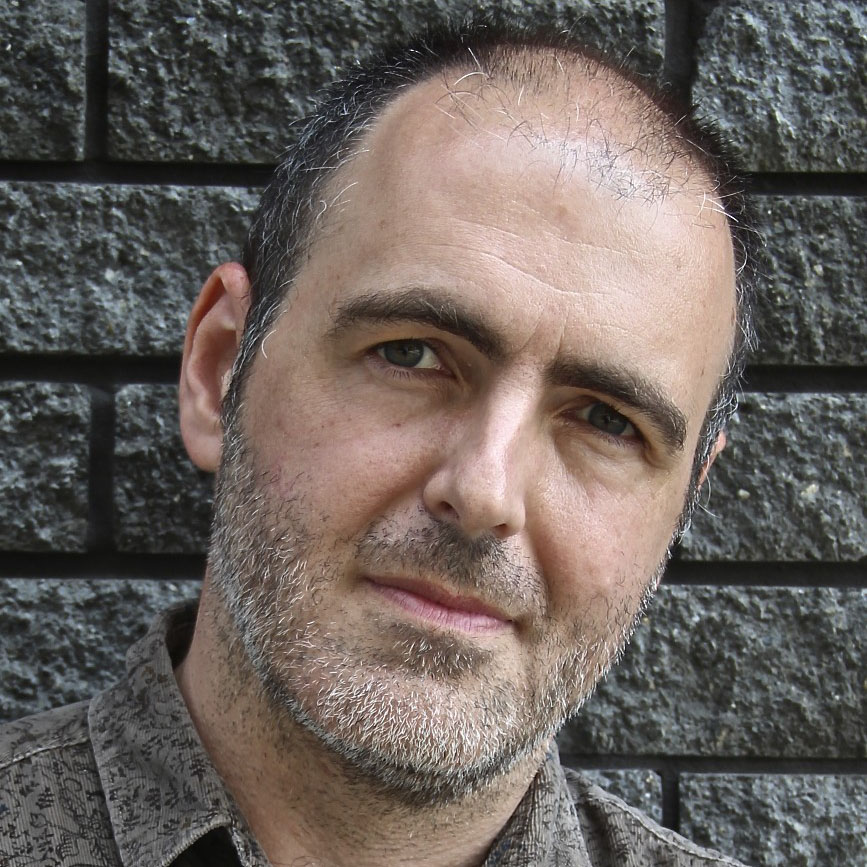
\includegraphics[width=5cm]{images/srp-mugshot} & 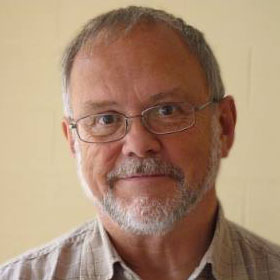
\includegraphics[width=5cm]{images/gdg-mugshot} \\
{\small steve.pettifer@manchester.ac.uk} & {\small graham.gough@manchester.ac.uk} \\
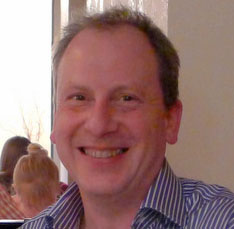
\includegraphics[width=5cm]{images/tljh-mugshot} & 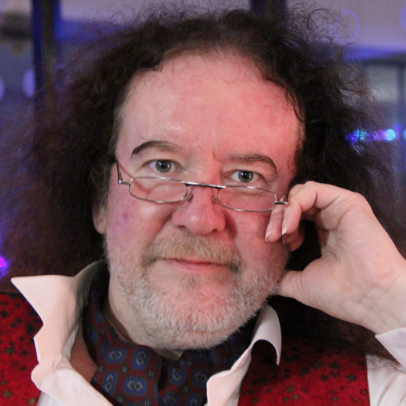
\includegraphics[width=5cm]{images/jtl-mugshot-2.png} \\
{\small toby.howard@manchester.ac.uk}  & {\small john.latham@manchester.ac.uk} \\
\end{tabular}
\end{table}

\section{Acknowledgements}
These notes are largely our own work, but have been inspired in places by previous lab exercises created by Pete Jinks, John Sargeant and Ian Watson. We're very grateful to Alex Day, Alex Constantin, Hamza Mahmud and Ben Mulpeter for test driving and debugging the exercises.

\renewcommand{\chaptername}{COMP10120 Lab Session}
\setcounter{chapter}{0}
\coursecode{COMP10120}
\chapter{Academic Malpractice Awareness}

\notesurl{desktop3}

\begin{note}
  This is where the script for the Academic Malpractice Awareness and Health and safety exercise goes

\end{note}


\chapter{Programming the shell}

\notesurl{desktop4}

\begin{note}
  This is where the script for the shell script exercise goes

\end{note}


\section{Git and GitLab}

During your time at school or college, you'll no doubt have written essays and assignments that took more than one session to complete, and you've probably experienced some annoyances associated with transferring the files containing your work between different machines. Perhaps you started writing on a PC at college, took it home to work on a bit more, and finished it off in a library or on a laptop in a cafe. You may have moved the file around using a cloud-based system like Dropbox or Google Drive, or perhaps you transported it around with you on a USB drive. In any case, it's more than likely that at some point you'll have got yourself muddled up working out which version of the file is the latest, or needed to undo some changes and had to remember which version of the file to go back to. If you've been unlucky, you may have lost important changes along the way, or got to a stage where it feels impossible to undo some unwanted change that you've made because it affects so many different parts of your work that you don't know how to remove their effects without messing up your whole document. If you've ever tried to work collaboratively on a project with someone else, you'll probably have found it quite hard to co-ordinate changes so that things you do don't trample on things that someone else is working on at the same time. 

These are all well-known problems associated with doing any kind of writing or project work that takes more than a few minutes to complete, where you're using multiple machines and/or are working with other people; and as you work on more complex projects over longer periods of time and with bigger groups, the bad news is that these problems all get worse. You can, to a certain extent, improve the situation by sticking to certain conventions, such as making regular backups of your work with particular kinds of filenames, or promising always to email your collaborators before you make a change to anything and emailing them again when you've finished your changes. But these informal `social agreements' easily collapse when you are tired or stressed, leaving you with a mess to clear up. The good news is that there are industry-standard ways of dealing with these problems, this session we're going to introduce you to the basics of version control using Git and GitLab. 

`Git' and `GitLab' are tools to help you manage change. Whether you're working on something on your own or as part of a team, a little effort spent learning how to use these tools now will save you significant amounts of pain and hassle later on. 

Git is a version control system, and is one of the most popular of the thirty or so different systems in use today. It is arguably one of the most powerful and flexible version control systems available, and this does mean that your first contact with it can be a little daunting; but if you follow our instructions carefully and don't get too hung up on the bits that we're having to skim over to keep things simple, you'll soon get the hang of things. 

GitLab is a web-based interface to git which makes it easy (at least, easier) to set up projects and teams for collaborative work. Mastering any version control system takes a long time, and you may find in the early days that using git feels as though it's more hassle than it's worth---but version control is a crucial skill for any modern computer scientist, and it's important that you get used to the principles right from the start of your degree. And trust us, at some point it is going to save you an enormous amount of trouble!

In combination git and GitLab provide mechanisms for:
\begin{itemize}
\item Safely moving files from one machine to another without losing changes in the process. You'll probably find this useful early on, and essential when you start working on your group project.
\item Tracking changes that you've made so that you can safely undo things that you later decide you don't want.
\item Keeping things under control when you're working with others on a shared piece of work.
\item Exploring the content of projects via a friendly web interface.
\end{itemize}

Today we're going to keep things as simple as possible, and are just going to use git and GitLab for some simple version control and for moving files between machines.

Before we can start to use the tools properly, there's some housekeeping that we need to do. 

\section{Configuring git}

Git has already been installed on the School's PCs, but you'll need to set up some things that are specific to you, before it will work sensibly. 

Fire up a terminal, and enter the following commands one by one:

\begin{ttoutenv}
$ git config --global user.name "[YOUR NAME GOES HERE]"
$ git config --global user.email "[YOUR UNIVERSITY EMAIL ADDRESS GOES HERE]" 
\end{ttoutenv}

Hopefully the purpose of these commands is self-explanatory; you're just telling git who you are and how to contact you by email if it needs to. The next bits of configuration are a bit more mysterious, and explaining them in detail would take up way more space than we have here; for now we'll just say that they set the default way in which git interacts with GitLab:

\begin{ttoutenv}
$ git config --global push.default simple
$ git config --global branch.autosetuprebase always 
\end{ttoutenv}

The next few instructions are optional, but make the output of git nicer to read, so we recommend you also do:

\begin{ttoutenv}
$ git config --global color.ui true
$ git config --global color.status auto
$ git config --global color.branch auto 
\end{ttoutenv}

and finally you should configure git to use whatever editor you've decided is your favourite at the moment, for example:

\begin{ttoutenv}
git config --global core.editor nano 
\end{ttoutenv}

Check that you've typed these correctly by using the command \ttout{git config --list}. You should see all the things you've entered just now, along with a few other bits of default configuration that were set automatically for you by the system (you can safely ignore these for now).

\section{Setting up GitLab}

Next we're going to set up GitLab. Point your browser at the School's installation of GitLab at:
\\
\url{http://gitlab.cs.man.ac.uk}
\\
and, on the `UoM Login' tab, log in with your University credentials. You should see GitLab's `dashboard' page and not much else (see Figure \ref{figure:GitLab-first-login}). Go to the `My Profile' section of GitLab using the icon at the top right of the page, and fill in any details about you that you're comfortable sharing with other students and staff within the School. At a minimum you should make sure that your Name and Email are set correctly; the other fields are optional. If you'd like your GitLab account to have an avatar image, you'll need to sign up for a \wikipedia{Gravatar}{Gravatar} account, which is a bit of a nuisance but not that hard.

\begin{figure}
\centerline{\includegraphics[width=15cm]{images/GitLab-first-login}}
\caption{First login to GitLab. \protect\circled{1} The GitLab logo (a sort of raccoon thing) will bring you back to the dashboard; useful if you get lost in GitLab's structure; \protect\circled{2} the user-profile allows you to add more information about yourself, and optionally connect up to Gravatar to give you a user icon; and \protect\circled{3} various ways to create a new project.}\label{figure:GitLab-first-login}
\end{figure}

\begin{diversion}{What about GitHub?}
You may have heard of a popular online git repository called GitHub, and be wondering why we don't just use that for your University work. GitHub is a fantastic resource, and is ideally suited for Open Source projects where you have lots of collaborators working together on a piece of Open Source code. GitHub's business model is that any project hosted on it must be Open Source, and visible for all users to see (not necessarily to edit). And of course, putting your solutions to lab exercises online for all to see is pretty-much the opposite of what we want to happen most of the time! It is possible to get non-open GitHub repositories set up, but GitHub quite reasonably charge for this service, and although it's possible to get non-open accounts for academic use, we decided it was cleaner to use our own installation of GitLab for Computer Science work, since we can hook it into the same authentication mechanisms that are used to control login to your other University services. The vast majority of features that you'll learn to use in GitLab can be easily transferred to other systems such as GitHub.
\end{diversion}

\section{Making your first project}

Git and gitlab both refer to collections of files that are being managed as `projects', because the most common case is that you are using them to control a software development project of some kind. There's no restriction on the size of a project really---it can have thousands of files in it, or just a few---and the layout of a project can mirror the kind of hierarchy that you'd have in your filestore, so you can have files and directories arranged however you like. We'll start off simple, and create a small project that represents the simple website you made in your previous lab sessions. Most version control systems use the term \concept{repository} to refer to the place where you store your files and the history associated with them. 

\begin{diversion}{Repositories}
Many version control systems such as \wikipedia{Subversion}{Subversion} have the idea of a central repository where you put your stuff, and from which you take copies of your files when you want to modify them. Git is rather different and is an example of what is called a \wikipedia{Distributed_revision_control}{Distributed Version Control} system; in the world of git you can have as many repositories as you like, each of which has a complete history of all the changes you've made. Instead of uploading and downloading from a central place, git has mechanisms to keep your repositories synchronised. 

In this case, however, we're using GitLab as a kind of `central repository' for your stuff. There's nothing special about the repository that GitLab manages from git's point of view really, except that we've set it up on a central server that's visible on the internet, so you can connect to it from anywhere using your University login details.
\end{diversion}

Select the `New Project' button from the icons at the top right (the one that looks like `+' symbol). Enter \ttout{aboutme} as the project name, and hit `Create project'. You'll see a page similar to Figure \ref{figure:GitLab-new-project}. Notice that the `Git global setup' section contains the commands that you used in the previous section to set up your git configuration; so you don't need to do that again. There are also two other sections of code on how to `create repository' or use `Existing Git Repo?' (`Repo' is a common abbreviation for repository). Ignore both of these for now and instead follow the instructions here (we'll come back to them later in this session). Notice at the top of the GitLab page a warning that `You won't be able to pull or push project code via SSH until you add an SSH key to your profile'---we need to fix that first. Click on the `add an SSH key' link (marked with \protect\circled{1} on Figure \ref{figure:GitLab-new-project}), which will take you to the SSH key upload page which looks something like Figure \ref{figure:GitLab-ssh}.

\begin{figure}
\centerline{\includegraphics[width=15cm]{images/GitLab-new-project}}
\caption{Creating a new project in GitLab. \protect\circled{1} You will need to use the  `add an SSH key' link to upload your public key before you can communicate between git and GitLab, and the URL given in \protect\circled{2} can be used from the command line to clone and push this project.}\label{figure:GitLab-new-project}
\end{figure}

\begin{figure}
\centerline{\includegraphics[width=13cm]{images/GitLab-ssh}}
\caption{Adding a SSH key to GitLab. Once you have used \ttout{ssh-keygen} to create the key, paste the text into the `Key' box; if your key is valid then the title will be filled in for you.}\label{figure:GitLab-ssh}
\end{figure}

You'll now need to set up a means of securely identifying yourself to GitLab from whichever machine you're using at the time; this is done by creating what's called a \concept{SSH key}. In a terminal, type:

\begin{ttoutenv}
ssh-keygen -t rsa -C "[YOUR UNIVERSITY EMAIL]"
\end{ttoutenv}

to create yourself a SSH key. When prompted `Enter file in which to save the key' just press return to accept the default, and the same for `Enter passphrase' twice.  For now don't worry too much about exactly what a SSH key is---we'll just treat it as a way of identifying yourself to the GitLab server. 

Look in a directory called \verb!~/.ssh! and you'll find two new files have been created called \ttout{id\_rsa} and \ttout{id\_rsa.pub}. The first of these is the \textit{private} part of the SSH key that's just been generated for you, and you should keep this secret. The second of these is the \textit{public} part of the key, and this is the bit you need to hand over to GitLab for it to be able to identify you. Use the command

\begin{ttoutenv}
$ cat ~/.ssh/id_rsa.pub
\end{ttoutenv}
% $
to display the contents of your public key. You should see something like:

\begin{ttoutenv}
  
  ssh-rsa  AAAAB3NzaC1yc2EAAAADAQABAAABAQDTfAF0KxG94oUJLUER5Ci5HaoEtdi8KI0S+
  iro3EvVkQebW2V3nCaCLAHLmgmINm/NFW5bvbUq7bu2CxFlVBEQqa1idZBLceXKRi1SFtG+
  EzFENyzZBsIDU0IhfQX4qyxgqe0A3ortyAwm2/+0neu74RT0YK3gQI+wyxsFFoCzbahiDJisK
  /vKmqvwowb/Rrl3OZpX9ZO3QA9lgILLVy3J4VpAhR+05MyuM/Bzh/pYk5NIQivedUEduIJXLOetj/
  UnxlH9WbEPEIiDPvzrkb3xI98rLRSlh2hH89nc1SUfVEhY62RQWN7sbXPu+fFck7Dom9wE/
  YAG66Dbl30OsmFh mister.noodle@manchester.ac.uk

\end{ttoutenv}

which starts with \ttout{ssh-rsa}, ends with your email address, and has a load of apparently random characters in between. Select this text (making sure you don't accidentally select any extra newlines or spaces either side of it) and 
Copy and Paste the whole of the SSH key into the `Key' box on the GitLab page. If you've done this correctly, GitLab will spot the email from your key and use this as the `Title' field, in which case just press the Save button. GitLab will complain if it's not a valid key or has extra spaces or newlines at this point; if you're stuck here grab a demonstrator to help you. 

Once you've uploaded your public key to GitLab, you're ready to put your first bit of content into the `aboutme' project that you've just created. 

Click on the GitLab logo at the top left of the GitLab page to get back to the dashboard, and select the `aboutme' project that you created a moment ago. 

You now need to add some content to the project to play with, so go back to a terminal window. If you happen to have copied the web pages that you created about yourself from the introductory labs onto your desktop machine, you're welcome to use those for the rest of this session; just make sure they are \emph{not} in a directory called \fname{aboutme} right now (rename the directory using \ttout{mv} if they are). Otherwise, use \cmnd{curl}{curl} to fetch the sample `mrnoodle' webpages again (these are the ones that you experimented with on your Pi).

The URL for these is 

\url{http://studentnet.cs.manchester.ac.uk/ugt/COMP10120/files/mrnoodle.tar.gz}

and you will need to use \cmnd{tar}{tar} to `untar' this bundle of files using the command

\begin{ttoutenv}
$ tar xvzf mrnoodle.tar.gz
\end{ttoutenv}

This will create a directory called \fname{htmlexample2}. 

Next we are going to \concept{clone} the (empty) project called \fname{aboutme} that you created in GitLab a moment ago onto your local filestore. Use the \cmnd{git clone}{git clone} command

\begin{ttoutenv}
$ git clone [REPO-URL-GOES-HERE]
\end{ttoutenv}

replacing [REPO-URL-GOES-HERE] with the full URL (it will start with \texttt{ssh} rather than the more common \texttt{http}) that you can see at the top of your GitLab aboutme project page, which is marked \protect\circled{2} in Figure \ref{figure:GitLab-new-project}. The URL will look something like:

\begin{ttoutenv}
ssh://gitlab@gitlab.cs.man.ac.uk:22222/mrnoodle/aboutme.git
\end{ttoutenv}

but obviously yours will be slightly different, so don't just cut and paste this one!

At this point, git will connect to GitLab, and make a copy of the empty \fname{aboutme} project in your filestore, creating you a copy of the project's repository. It should complete with the message `warning: You appear to have cloned an empty repository.' This is fine, because we know it's an empty repository at this stage.

\begin{diversion}{Connecting git to GitLab}
We could have set up our new project a different way, by initialising the project in our home directory (using \ttout{git init}) and then connecting that up to GitLab, but the later step of connecting a newly init'd repository with a project you've made in GitLab is a little fiddly, so it's slightly easier to explain what's going on the way we've done it here. We'll do it the `other way round' by starting with a directory full of files and sending that to GitLab later on in today's session. 
\end{diversion}

Change into the newly created \fname{aboutme} directory, and use \cmnd{ls}{ls -a} to see what's in there. It should be an empty except for a \concept{hidden directory} called \fname{.git}, which is where git is going to put its own administrative files. Feel free to take a look inside the \fname{.git} directory if you're interested, but please make sure you don't modify anything in there, otherwise you may get into a mess later on. 

Now copy the files from \fname{htmlexample2} (or your own website's directory) into \fname{aboutme/}. If you're using the default Mister Noodle ones, you'll have three files: one HTML, one .jpg and one .png (of course if you're using your own files, these may be different). 

Before we start adding these files to the project, let's see what git thinks the current status of that directory is. Use the \cmnd{git status}{git status} command 

\begin{ttoutenv}
$ git status
\end{ttoutenv}

and you'll see a message from git that, amongst other things tells you that there are `untracked files' (these should appear in red). 

So we need now to tell git which files we want it to track for us. We need to \cmnd{git add}{git add} \emph{each of the files in that directory} like this:

\begin{ttoutenv}
$ git add [FILENAME]
\end{ttoutenv}

% $

replacing [FILENAME] with each of the file names in turn. Once you've done this, run \ttout{git status} again, and this time you should see that there are a list of `Changes to be committed' and all the files that you'd just added should appear in green. 

Now git knows which of the files in this directory you want to track (which in this case is all of them), we want to do our first \concept{commit}, which tells git that we've made a set of changes that we want to keep together: in this case the `changes' are to create the files in the first place; later on we'll go through a similar pattern of \ttout{git add} and {git commit} whenever we've done a set of changes that we think we are happy with. 

The \ttout{-m "Initial Commit"} part of the commit line gives git a label to associate with this particular commit, and it's traditional to put the message `Initial Commit' the first time you tell git about a new set of files. In future you'll be putting text here that summarises in human-readable form what changes you've made in this commit, but more on that later.

\begin{ttoutenv}
$ git commit -m "Initial Commit"
\end{ttoutenv}

Don't worry about what git's response means here, that will become clear as you learn more. Type \ttout{git status} once again and if everything has gone to plan you should see the response

\begin{ttoutenv}
# On branch master
nothing to commit (working directory clean)
\end{ttoutenv}

If you get a different message here, then something has gone wrong in one of the previous steps; don't worry, just call a demonstrator to help out. 

So to recap: in GitLab we've created a project repository called `aboutme' ready to accept some files, and we have then \concept{cloned} this empty repository into your home directory (essentially making an exact copy of it). We then created some files in our local directory, used \ttout{git add} to tell git that we wanted to track them, and then \ttout{git commit} to tell git that those files in their current state form a sensible collection. 

Use the web-browser to go back to your \ttout{aboutme} project page on GitLab. You'll see that nothing has changed on the server yet; that's because \ttout{git add} and \ttout{git commit} only make changes to the git repository \emph{that's on your local machine}.

The next step is to send a copy of these files to the GitLab server for safe keeping, and so that you can fetch them back from, say, your home machine. In git terminology, synchronising changes \emph{from} one repository (in this case your local one) \emph{to} another (in this case the one hosted on the GitLab server) is called a \concept{push}. 

Doing this is simple; just type:

\begin{ttoutenv}
$ git push
\end{ttoutenv}

from within the \fname{aboutme} directory, and git will connect to your GitLab account, and copy the files and their revision history over on to the server for you (git knows where the files should go, because it's remembered where you got them from in the first place by storing that information somewhere in the hidden \fname{.git} directory you saw earlier, so you don't need to keep reminding it). 

Refresh your browser's GitLab project page again, and this time you should see a message saying that you have `pushed a new branch' (don't worry about the use of the word `branch' here---it's a reference to the fact that git can cope with multiple sets of changes happening in parallel and coming from different places). If you're not seeing that, summon a demonstrator to get help. 

If you now look at the `Files' menu in GitLab's page for your \fname{aboutme} project, you should see all the files that you added, committed and pushed; clicking on the individual file names should show you their content, so you can see what their latest status is. 

Look at the header of the table that contains your files, where it says `Name', `Last Update' and `Last Commit', and next to the `Last Commit' you will see a string of characters containing letters and numbers; this is a unique string that identifies your commit, and you can use it later to revert files back to the state they were in when you did that particular commit. Note that some times you'll see longer versions of this string (for example later when you use the \cmnd{git log}{git log} command; as long as you give git enough characters for it to be able to uniquely identify a particular commit that you've made, git will be happy. So usually you don't need to use the long version).

Back at the command prompt, fire up an editor and make a small change to the HTML file; it doesn't really matter what the change is as long as it is something you can recognise as being different from the original version.

Then type \ttout{git status} again, and you'll see that git knows that you have modified that file since your last commit. Lets say that you want to remember this change next time you do a commit; you need to tell git this using 

\begin{ttoutenv}
$ git add [NAME OF THE FILE YOU CHANGED]
\end{ttoutenv}

so do this, and then run \ttout{git status} once more to check that git now knows that you want it to remember the changes to this file since the last commit. 

It's important to understand that you need to run \ttout{git add} whenever you want git to recognise a change you've made to a file; if you make changes \emph{after} having run \ttout{git add}, git will not take those into account unless you run \ttout{git add} again to tell it that you really did mean to make those changes. You don't have to do it after every edit; just after edits that you want to keep. 

In git terminology, this process is called \concept{staging}; think of it as `setting the stage' or `getting things ready' to be put into your project's history. 

But for now, let's assume that this is the only change you need to make right now, and that you want  git to remember this change as part of your project's history; the command for this is called \cmnd{git commit}{git commit} Type

\begin{ttoutenv}
$ git commit -m "[SOME WORDS THAT DESCRIBE YOUR CHANGE]"
\end{ttoutenv}

replacing the text in braces (and the braces themselves) with something that would help you remember what you did if you needed ever to check in future. 

At this stage, your change has been recorded in the \emph{local} git repository in your filestore. To push this change over onto the GitLab server, you just need to type

\begin{ttoutenv}
$ git push
\end{ttoutenv}

once more, and everything will get synchronised with your GitLab account.

Go back to the GitLab page for this project in your browser, and look at the status of the project's files now and you should see this change reflected there. Notice now that the unique identifier for your Last Commit has now changed, and that whatever comment you put in on the commit line also appears in the table to remind you where you're up to. 
Notice also that only the file you modified has been updated; the others will still say `Initial Commit' against them, since nothing will have changed there since your first commit. 

Experiment a bit now by editing the files again (perhaps use the Gimp application to change the images as well as editing the HTML file), and practise using \ttout{git add}, \ttout{git commit} and \ttout{git push} to record these changes and send them to the GitLab server. At each stage, use \ttout{git status} to confirm that git is reporting what you'd expect it to, and look again at the GitLab page in your browser to make sure that makes sense at each step too. 

When you're happy that you understand these three commands, you're ready to move on to the next step.

\section{Keeping files synchronised between two repositories}
Imagine now that you've gone back home and want to retrieve the latest files you've been working on. Don't go back home though, there's still more work to do in the lab! 

In git terms, what you want to do is to get a copy of your project repository on your home machine. For now we'll simulate that by just making a new directory in your CS filestore, and cloning your project into there. 

In your home directory make a new directory called \fname{gittest}, and \ttout{cd} into it; we're going to use this to pretend that you're now in a different machine that can't see your computer science filestore directly. Assuming that you've got git installed, and have a SSH key on your home machine, the process would be identical.

Use the same \ttout{git clone} command that you used earlier to get yourself a \emph{new copy} of your \fname{aboutme} project from GitLab; you should then find a copy of \fname{aboutme} has appeared in your current working directory. Unlike previously where \ttout{git clone} created an empty directory for you (because you'd not put any files into the project at that stage), you should now find that this new \fname{aboutme} contains the latest versions of the files from your other version of the project.

Use the \cmnd{git log}{git log} command to see what the history of this project is; you should see all the commits that you've made so far, along with the descriptions gave for what the commits meant. 

Make another change to one of the files, then \ttout{add}, \ttout{commit} and \ttout{push} that change to the GitLab server's repository. Check that you can see these latest changes in the GitLab web pages.

Go back to your \emph{original} \fname{aboutme} directory (imagine that you're now back at the University doing some work in the lab, and want to pick up the changes you made to your stuff when you were at home). This time you want to do the opposite of a \ttout{push} in order to bring your local copy up to date with whatever is on the server. The command to achieve this is called, not unreasonably, \cmnd{git pull}{git pull}, so run that now, and you should find that you once more have an up-to-date version of your work. Hurrah!

Practice making changes in one or the other of the two \fname{aboutme} directories that you've made (imagining that one of them represents a directory on your machine at home), and make sure you're comfortable with the cycle of using \ttout{add}, \ttout{commit} and now both \ttout{push} and \ttout{pull} to move changes `between machines' via the GitLab server.

\section{Reverting a file to a previous version}

Let's say you've messed one of your files up in a recent change, and want to go back to a previous version. You need to find the unique number that's associated with the commit that had the version you want. Use \ttout{git log} to see your change history and pick one of the commits that you've made already (your comments should tell you what you did in that commit; if they're not helpful, you might want to think about what kind of comments you're using!). Find the long number associated with that commit, and type

\begin{ttoutenv}
$ git checkout [UNIQUE NUMBER FOR COMMIT] [NAME OF FILE YOU WANT TO REVERT]
\end{ttoutenv}

If you've got this right, git will just return you to the command prompt without complaining; if you get an error or warning that you don't understand, grab a demonstrator. 

Look at the file you've just checked out, and you should see that it's one of the old versions you had previously. You've now got the choice of continuing to work with the file you've just reverted (you'll need to \ttout{add} it back later before doing a commit), or throwing it away and picking another version. If you want to discard it and get back to the latest version of that file, just use \ttout{git checkout HEAD [NAME OF THE FILE]} to get back to the most recent edits (here `HEAD' just means `the most recent version that I've committed').


\section{A Recap}

Before moving on to do some `real' stuff with git and GitLab, let's quickly revisit some of the key ideas.

\begin{enumerate} 
\item When you're working with git, the files and directories that you're editing are held locally in your filestore just like any other files or directories. In git terminology this local copy is called your \concept{workspace} or \concept{working copy}. 
\item When you first want to tell git to track a file fore you, or after you've modified a file with a change that you want git to later remember when you do a commit, you use the \cmnd{git add}{git add} command to \concept{stage} the file. This records the current status of the file temporarily in what is called the \concept{staging area} (or is sometimes referred to as the \concept{index}). The content of staged files only get recorded in the project's history the next time you run \cmnd{git commit}{git commit}. 
\item When you want to record a set of changes together, you use the \cmnd{git commit}{git commit} command, which takes any staged files and records their state in the \concept{local repository}, and the commit message in the project's log.
\item If you want to synchronise your local repository with another repository elsewhere (referred to as the \concept{remote repository} or more correctly as the \concept{upstream repository}), you can either \cmnd{git pull} changes \emph{from} the upstream repository, or \cmnd{git push} them \emph{to} the upstream repository. In our case, we're using GitLab as your upstream repository.
\end{enumerate}


\subsection{The lifecycle of a file under git's control}

It's also important to be clear about the \emph{lifecycle} of a file that's being looked after by git. This is illustrated in Figure \ref{figure:git-file-life-cycle}. A file \protect\circled{1} will start off life being \concept{untracked}, i.e. it's a file that git knows nothing about. Using the \cmnd{git add}{git add} command, you can ask git to track the status of the file, at which point the file is \concept{staged} \protect\circled{2}. You can them \cmnd{git commit}{git commit} this file, and any others that have been staged, which makes a copy of them in the project's local repository, and returns their status to being \concept{unmodified} \protect\circled{3} because now the file's content is in sync with the version you've just committed. Editing the file causes it's state to change to \concept{modified} (i.e. `not the same as what's in the latest commit') \protect\circled{4}; and you can use \cmnd{git add}{git add} to put the file back in the staging area ready to commit again. This cycle is repeated until the project is finished. 



\begin{figure}
\centerline{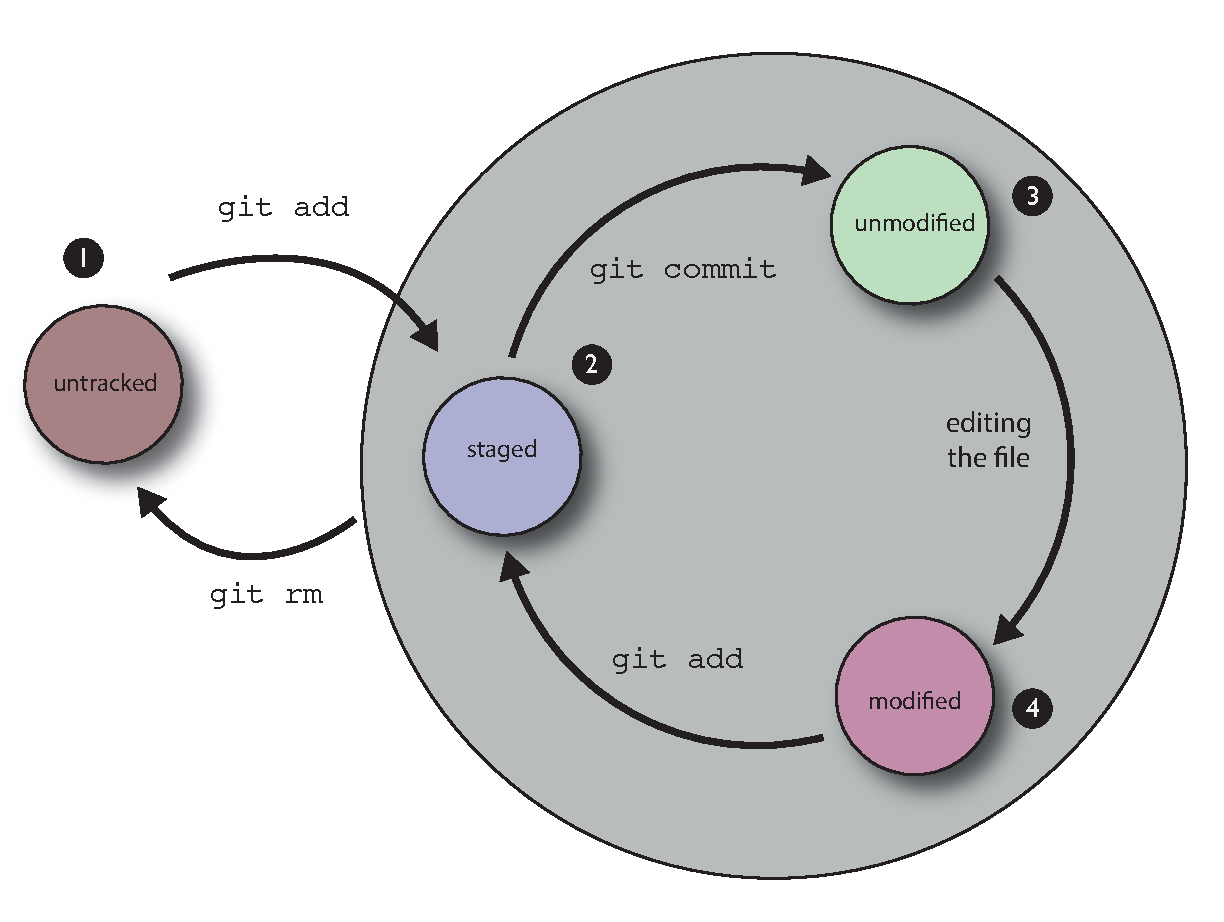
\includegraphics[width=15cm]{images/git-file-life-cycle}}
\caption{The life cycle of a file under git's control.}\label{figure:git-file-life-cycle}
\end{figure}

You should now have enough knowledge to be able to do three things with git and GitLab.

\begin{enumerate}
\item Use them together to safely move files between different machines, knowing that your content will be backed up in GitLab, and also that the history of changes that you've made will get preserved nicely.
\item Use GitLab as a handy way of looking at the content of files in your project (for example, if you only have access to a web browser and not a machine with a command-line interface).
\item Use git to safely revert files to previous versions if you've got yourself into a pickle. 
\end{enumerate}

Git and GitLab together can do much more than this, and will be invaluable tools when you start to use them for your group project work. But it's important right now that you just get into the habit of using them on your own to manage your own individual work; it'll make the few extra things that you will need to learn to use them as a group-tool much easier.

And yes, you'll probably think that using git is more hassle than just shoving all your stuff into a cloud based system and hoping for the best; but please trust us, by practising this stuff now you're not only developing an essential skill for your future careers, you will find at some point soon that it saves you a lot of pain and hassle. 


\subsection{Basic git commands again}

\begin{figure}
\centerline{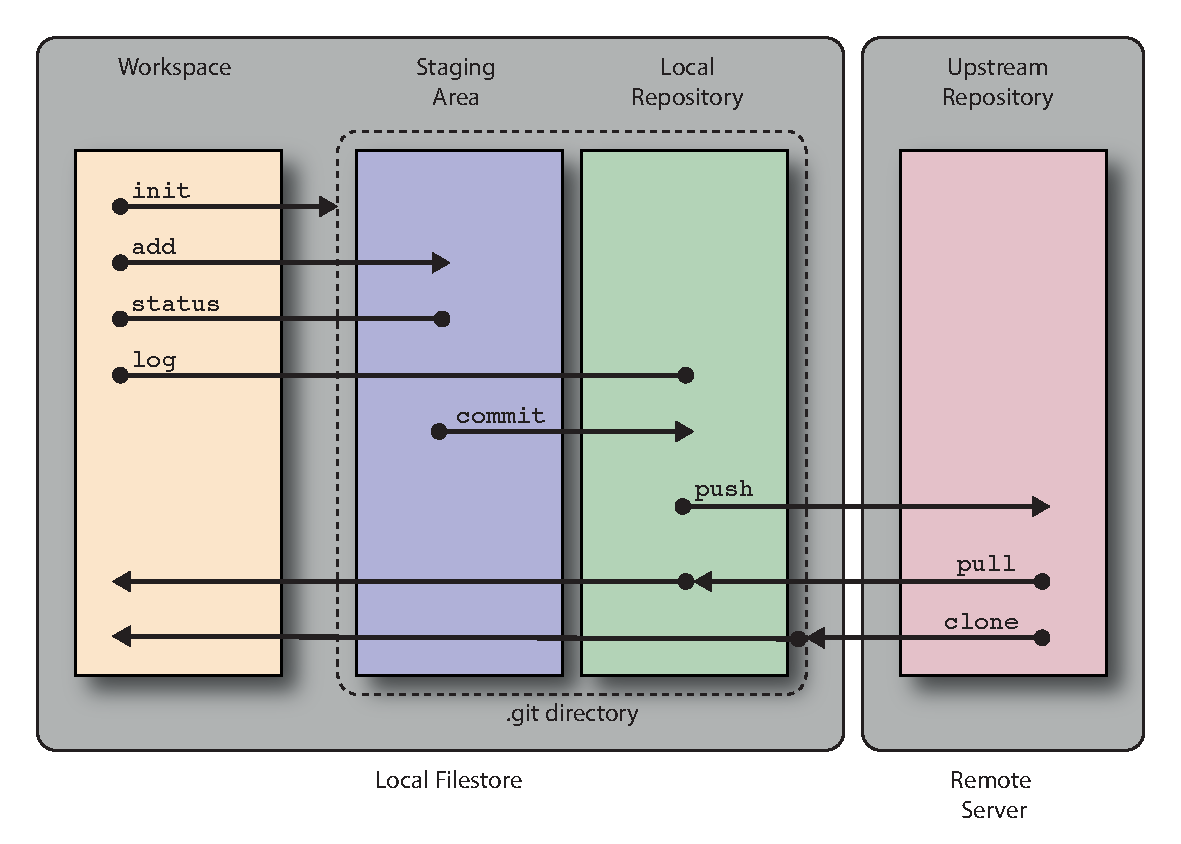
\includegraphics[width=15cm]{images/git-commands}}
\caption{Basic git commands and their interaction with the various repositories}\label{figure:git-commands}
\end{figure}

Figure \ref{figure:git-commands} shows how the various commands we've looked at so far interact with the different repositories used by git. 

\begin{itemize}
\item \ttout{git init} creates an empty local repository in the current working directory. 
\item \ttout{git add} `stages' a file by adding the \emph{current content} of new or modified files to the staging area. 
\item \ttout{git status} gives you the status of files in the workspace and staging area. It will tell you which stage of the file life cycle (Figure \ref{figure:life-cycle} each file is in. This command doesn't know anything about the status of any upstream repositories.
\item \ttout{git log} gives you the commit history of your project, giving you the unique identifiers and messages associated with each commit.
\item \ttout{git commit} bundles together all staged files, and commits them to the local repository along with a message describing the change. Remember, this doesn't automatically push your changes to the upstream repository, it's only makes the changes locally. 
\item \ttout{git push} updates the upstream repository with any commits that have happened since the last push. If the upstream repository has changed in the meantime (for example, because someone else has pushed new changes before you), this command will fail with an error to prevent you accidentally over-writing something else.
\item \ttout{git pull} fetches the latest changes from the upstream repository, and merges them into the local one, updating the workspace versions in the process.
\item \ttout{git clone} downloads a repository from a server.  
\end{itemize}


\exercisess{Submitting your progress so far}

In your COMP10120 directory, create a new subdirectory called \fname{ex4}. In your \fname{aboutme} directory, run the \cmnd{git log}{git log} command, and redirect its output to a file called \fname{\$HOME/COMP10120/ex4/aboutme.gitlog} using the command

\begin{ttoutenv}
$ git log > $HOME/COMP10120/ex4/aboutme.gitlog
\end{ttoutenv}

Then change into the \fname{ex4} directory and check that the contents of \fname{aboutme.gitlog} is what you expect. This file is one of the things that \ttout{submit} will pick up when you run it at the end of the lab sessions; the \emph{exact} contents of the file don't matter, but we will expect it to show the history of your aboutme project, and to have some sensible commit messages. 

\section{Putting real work into git}

So far we've experimented with some throw-away webpages in your \fname{aboutme} directory. Now it's time to put some real content into git and GitLab.

\exercisess{Putting COMP10120 under version control}

Make a new project in GitLab called COMP10120. 

This time, because you already have some content that you want to put into a project (rather than starting `from scratch' like we did earlier), go to your \fname{COMP10120} directory and type \ttout{git init}. This should respond by saying that it has `initialized empty Git repository'. Now look through the different files and directories that are in \fname{COMP10120}, and use \ttout{git add} to add \emph{only those files that you want git to track for you}. What's important here is that you only add files that are your original source files (for example, those that end with .tex), and not things which are automatically generated by tools such as the .pdf or .aux files created by LaTeX.

Use \ttout{git status} regularly to check that the files you want to track, and \ttout{only} the files you want to track have been added to git's list, and then use \ttout{git commit} to make your initial commit. 

Next you'll want to synchronise your local repository with the one in GitLab. This is a little more fiddly than just doing a `clone' like we did earlier, but just follow these instructions and all will be well.
 
Look back at the aboutme project's page on GitLab, and find the COMP10120 project's URL (again, this is labelled with \protect\circled{2} in Figure \ref{figure:GitLab-new-project}).

Then enter the following command, copy-and-pasting the URL from the web page into the appropriate bit of command line:

\begin{ttoutenv}
$ git remote add origin [GitLab-URL-GOES-HERE]
\end{ttoutenv}

This makes an association between the repository that you've created in your filestore, and the project in GitLab.

Finally to send this first version of the repository over to the GitLab server, enter

\begin{ttoutenv}
$ git push -u origin master
\end{ttoutenv}

which should respond with some variation of 

\begin{ttoutenv}
Counting objects: 3, done.
Writing objects: 100% (3/3), 216 bytes, done.
Total 3 (delta 0), reused 0 (delta 0)
To ssh://GitLab@GitLab.cs.man.ac.uk:22222/mister.noodle/aboutme.git
 * [new branch]      master -> master
Branch master set up to track remote branch master from origin by rebasing.
\end{ttoutenv}
 
Check using your browser that GitLab has now received the right versions of your files for the COMP10120 project.

The the same output redirection mechanism we used a moment ago to record the output from \ttout{git log} for the COMP10120 project into a file called COMP10120.gitlog in your \fname{COMP10120/ex4} directory so that \ttout{submit} can find it later. Once again, the \emph{exact} contents of the file don't matter as long as it is a sensible representation of your commit history for this project.

If this has worked, then move on to the final exercise. If there are any problems, or you're at all unsure about what's going on, find a demonstrator to help you. 

\exercisess{Putting your COMP16121 exercises under version control}

To finish off this laboratory session, create a project for COMP16121 and put all the appropriate files under git's control. Remember again -- you only want to put \emph{source} files or files that you've created yourself into git, not ones that are the output of the Java compiler or any other program.

Now this time there are probably a lot more files to worry about, and you might not want to go through them one by one \ttout{git add}ing them each individually. Instead you could use something like this to add them to the staging area:

\begin{ttoutenv}
$ cd ~/COMP16121
$ git add ex*/run-alltests
$ git add ex*/task*/run-tests
$ git add ex*/task*/*.java
\end{ttoutenv}

Check that only the files you want to add have now been staged using \cmnd{git status}{git status}, and get help from a demonstrator if the result isn't what you expected.

When you're happy that the staged files are the correct ones, use \ttout{git commit} to commit them, and then save the git log to a file called \fname{COMP16121.git} in your \fname{COMP10120/ex4} directory (this is your final submittable deliverable for today's session). 

When your Java code is all safely in GitLab and you have three log files recorded in {COMP10120/ex4}, you're done for today (but if you have a machine that you can use at home, please take the opportunity to see if you can clone the projects you've made today onto that to experiment further). 


\section{Using Git for real}

It's really important that you're comfortable with basic git usage, and you should make sure that from now on any work that you do in \emph{any} of the labs (not just in COMP10120) is put under git control. This will make it much easier for you to work on files from home, and may also get you out of trouble if you get carried away with the \cmnd{rm}{rm} command at some point, because you will have some backup stored in GitLab (every year, someone will accidentally delete important work; don't be that person---put everything you do in GitLab and you can't go too far wrong!)

\section{Other git learning resources}

Git is widely documented and discussed online, and there are loads of excellent resources (and of course quite a few duff ones!) that you can use to improve your understanding of using source code control systems generally, and git specifically. In particular:

\begin{itemize}

\item Schott Chacon's `Pro Git' book is available online for free and is an excellent guide to git from the very basics to much more advanced use than is covered in today's lab session. It is well worth a read. \url{http://git-scm.com/book}

\item There's a very useful quick-reference site at \url{http://gitref.org}

\item Andrew Peterson's Interactive Git Cheat Sheet is also a very useful reference tool, though probably only makes sense when you are reasonably familiar with git. \url{http://ndpsoftware.com/git-cheatsheet.html}
\end{itemize}

\section{Git `Best Practice'}

These are some basic principles that you should keep in mind when you're using git (or any version control system, really). They are very much \emph{principles} rather than rules; things that you should aspire to do unless there are very good reasons not to. On the whole sticking to these means that you'll be able to use source code control systems more effectively, and will avoid some of the pitfalls that can trap you if you're careless. 

\begin{enumerate}
\item \textbf{Commit \emph{related} changes}. A commit should really represent one conceptual change to your work. This may (and probably will) involve changes in several files, but ideally you should be able to describe what the commit means in a single sentence. For example, if you are fixing more than one bug, you should probably be doing more than one commit. If you find that the message you'd be putting into the log to describe the change involves the word `and', you may want to think again (for example, a change that `fixes the startup bug, and improves the colour scheme in the logo' should really be two separate commits). The universe won't grind to a halt if you do this, but it does mean that in future it would be harder to change your logo colour without undoing the startup bug fix as well.

\item \textbf{Commit frequently} Making lots of smallish commits helps avoid the problem described above, and also makes it easier to undo changes if you find something bad has happened. 

\item \textbf{Avoid committing half-finished things}. Try to make sure that when you do a commit it represents exactly one fully finished change; a commit that's only half a change is much harder to describe in a commit message, and harder to understand later when you come back to your work. This is especially important when you are working in collaboration with other people; a half-working (which of course means half-not-working!) commit means that your collaborators get a broken system to work with, and that won't make you popular.

\item \textbf{Write meaningful commit messages}. Its tempting sometimes to abbreviate or put junk into your commit messages to save hassle at the point of committing, but this will come back to bite you later; your collaborators will not appreciate this at all either. Ideally the first line of your message should be a short (around 50 character) description of the change, so that it can fit onto a single line of a terminal when you look at the log. You can then add a blank line, followed by a more comprehensive description of what changes you've made (why did you make this change? how is it different from before?)


\end{enumerate}

\section{Marking Scheme}

You can view a copy of the marking scheme used by submit and labprint at:

\url
{
http://studentnet.cs.manchester.ac.uk/ugt/labprint/readms.php?unit=COMP10120&ex=ex4.xml
}


















% \usepackage{graphicx}
% \usepackage{palatino}
% \usepackage{url}
% \usepackage{hyperref}

% %\usepackage{a4-mancs}

% \usepackage{handout}

% \begin{document}
\newgeometry{a4paper}
\setlength{\parskip}{\parskipdefault}
\setlength{\parindent}{\parindentdefault}

\chapter{Report writing and Digital Typography}
\begin{refsection}
  
  \minitoc

  \notesurl{latex-exercise}

\section{Introduction}

\LaTeX\ is a document preparation system that is fundamentally
different to anything that you are likely to have seen before. It's
used worldwide by publishers, academics and scientists.

\LaTeX\ was written by Leslie Lamport, an American computer scientist now working at Microsoft Research.  It's actually built on top of another system called \TeX, a computer typesetting system designed by one of the world's most influential Computer Scientists, Donald Knuth of Stanford University. Knuth has said that he designed \TeX\ for `the creation of beautiful books---and especially for books that contain a lot of mathematics.'\citep{knuth1984}. Figure \ref{figure:knuthlamport} shows what these eminent men look like.

  
So what's the purpose of \LaTeX ? It's purely a layer of software to make \TeX\ easier to use in everyday situations. This is a good idea, because although \TeX\ is amazingly powerful, it operates at a very low-level, which makes it hard for non-expert users.

\begin{figure}[hb]
  \centering
     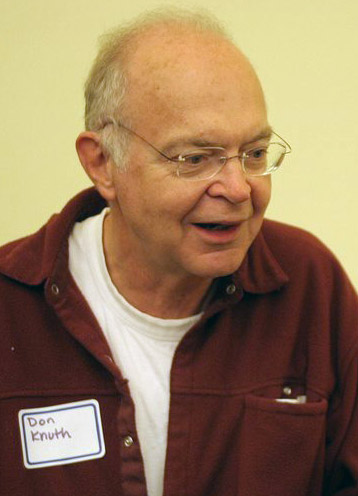
\includegraphics[height=6cm]{images/knuth.png}
\quad\quad  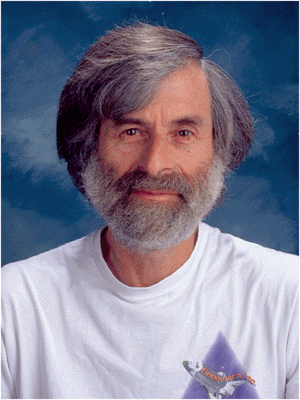
\includegraphics[height=6cm]{images/lamport.png}
\caption{Don Knuth and Leslie Lamport.}\label{figure:knuthlamport}
\end{figure}

\subsection{Pronunciation}
\label{sec:pronunciation}
  The name \TeX\ is intended by its creator to be pronounced with the final consonant as in the word loch or the name Bach, but English speakers often pronounce it like the first syllable of technical. The first syllable of \LaTeX\ is pronounced as in 'lay'\footnote{The Greek prefix `tex' means `art' as well as `technology', so it's a very nicely chosen name for a piece of software that produces such beautiful output. Knuth explained \citep{knuth1984} that one should ``pronounce the X of TeX as a Greek chi, not as an `x', so that TeX rhymes with the word blecchhh.''. We're not too sure that helps much, unless you are confident in your pronunciation of the word `blecchh'. Maybe it's an American thing.}.


\section{Why \LaTeX?}
\label{sec:why}
 Before we go any further, why do we think \LaTeX\ is important for you---a Computer Science student---to know about? Here are some reasons, in no particular order.

\begin{itemize}
\item \LaTeX\ and \TeX\ are superb examples of Computer Science in action. \TeX\ was designed by Knuth from \concept{first principles}---in other words, from scratch.  \TeX\ is actually a programming language, and \LaTeX\ is a set of functions defined in the \TeX\ language. The \TeX\ `compiler'  is  written in \wikipedia{WEB}{WEB}, a mixture of documentation written in TeX and a Pascal subset in order to ensure portability; it reads a \TeX\ program and outputs documents. \TeX\ is completely self-contained and designed to be portable to any computer architecture. (For example, it implements its own stack and heap (with garbage collection), and it does fixed-precision arithmetic). 
\item \LaTeX\ is a new, interesting, way for you to think about preparing documents. 
\item \LaTeX\ has a practical advantage for the writer, in that it helps you think more about \emph{what} you want to write, rather than worrying about \emph{how it looks}.
\item \LaTeX\ is a powerful tool for professional scientific documentation, and as a Computer Scientist, you should know about it.
\item \LaTeX\ files are just plain text, so can easily be created programatically. For example,  the slides used for \courseunit{COMP16120} are generated automatically from the source of John's book; both are typeset using \LaTeX. The program \texttt{labprint} also produces its output using \LaTeX, using information drawn from XML configuration files and ARCADE.
  
\item Using \LaTeX\ is actually quite satisfying, and the quality of its output may surprise you.
\end{itemize}

In this lab session you are going to write several short  documents using \LaTeX. You could also write brief notes in your logbook about how \LaTeX\ works and what commands you used inside the source of your documents.

Please complete the exercises in your \fname{COMP10120/ex3} directory. When you have completed as much as you are going to do, you should run \texttt{submit} and (when next in the School) \texttt{labprint}.

\section{Some history: printing mathematics}

Mathematics is hard to print, on paper, and on the Web (many websites resort to GIF or JPG images of maths formulae, which usually look horrible. \wikipedia{MathML}{MathML} provides another approach, but it is not yet widely used).

In the days before computers, books and newspapers were printed with \wikipedia{Movable_type}{movable type}, made from lots of little blocks of metal each with letters, numbers and symbols standing in relief, which, when inked, left an impression on the paper (see Figure \ref{figure:movabletype}). The job of the printer (the printer here, of course, being a person, not a bit of electronics) was to gather together all the blocks in the right order between two horizontal strips of wood to create a line of the document, and then to assemble all those lines from top to bottom of a page. Thus the term \wikipedia{Type_setting}{type setting}: an incredible task, when you think about it. In the printer's workshop, by the way, the blocks of metal were stored between jobs in wooden boxes called \concept{cases}. Letters like a, b and c were stored in one case; letters like A, B, and C were stored in a case sitting on top of that. So, a lower case, and an upper case. These terms may ring a bell.

\begin{figure}
\centerline{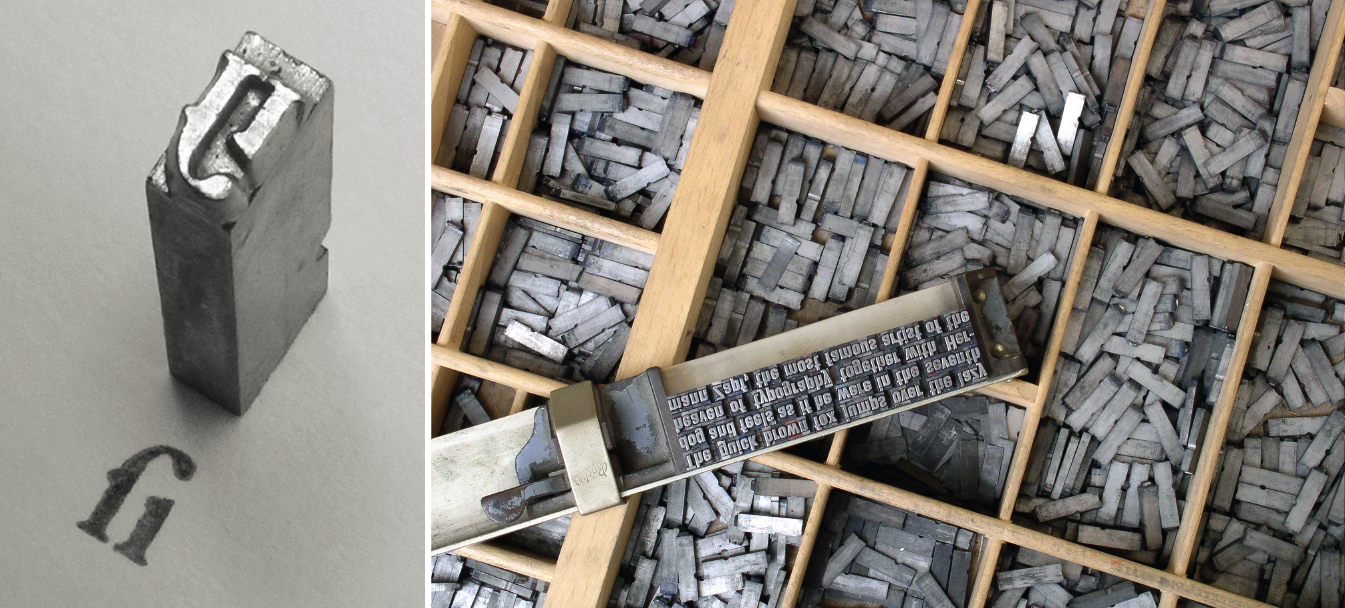
\includegraphics[width=12cm]{images/movable-type.png}}
\caption{On the left, a piece of cast movable type in the Garamond font. On the right, a case of cast metal type pieces and typeset matter in a composing stick. The text reads `The quick brown fox jumps over the lazy dog and feels as if he were in the seventh heaven of typography together with Hermann Zapf, the most famous artist of the' (this document is typeset in a font called Palatino, created by Hermann Zapf. You may have also seen 'Zapf Dingbats' in the font lists of various desktop applications. Now you know why.)} \label{figure:movabletype}
\end{figure}

As technology progressed, machines controlled by typewriters would mechanically juggle the blocks into the right order. This conceptual model is the basis on which \TeX\ operates. Only now, the metal blocks are little pieces of data, arranged into data structures. 

The one thing that traditional printers hated was dealing with the typesetting of mathematics, and they would charge extra to do it. It was incredibly fiddly: to get the equations looking right they had to squeeze in extra bits of metal horizontally and vertically. 

When computers entered the printing world, attempts to print mathematics were limited by the printing technology available. It took a long time to reach the point where computers could typeset mathematics beautifully, and that was the outstanding achievement of Knuth's \TeX.

Let's look at a quick example of the quality you get from \LaTeX, with a very simple formula that you'll recognise:

\[ x = \frac{-b \pm \sqrt{b^2-4ac}}{2a} \]
%
We'll revisit how \LaTeX\ typesets mathematics in Section~\ref{mathssection}.

\section{To WYSIWYG or not to WYSIWYG?}
Up until now, you have probably used wordprocessing applications such as Microsoft Word to create essays, letters and other (probably fairly short) documents. You most likely know that the majority of modern word processors use a paradigm called WYSIWYG, or What You See Is What You Get, which means that you can modify the visual style of the document you're working on by selecting the relevant bits, and then choosing different attributes such as font size or colour using a GUI. In many ways this seems like such a sensible and obvious way of doing things, that you might be wondering why it even has a special name. The reason is a historical one: in the early days of computing, long before graphical window managers became the norm, and when all you could display on screen was fixed-width ASCII text in whatever the system's default font was, wordprocessors (e.g. Figure \ref{figure:wordperfect}) only allowed you to format documents by using special sequences of characters to cause particular effects. But these effects were only visible when the document was printed. So if you wanted a word to appear in \textbf{bold text}, in the wordprocessor you might write something like \texttt{[bold]hello world[/bold]}: what you saw on screen was \emph{not} a direct reflection of what appeared on the printed page. If you've written any HTML, however, this process of \concept{marking up} text may be familiar, see, for example Figure~\ref{figure:helloworld}. As computers moved to displays able to draw things other than raw characters on screen, wordprocessors became capable of using multiple fonts and styles, as well as graphics, and a new generation of applications appeared where what you saw on screen \emph{was} an accurate reflection of how it would appear when printed: what you see (on screen), is what you get (on paper). 

\begin{figure}
\centerline{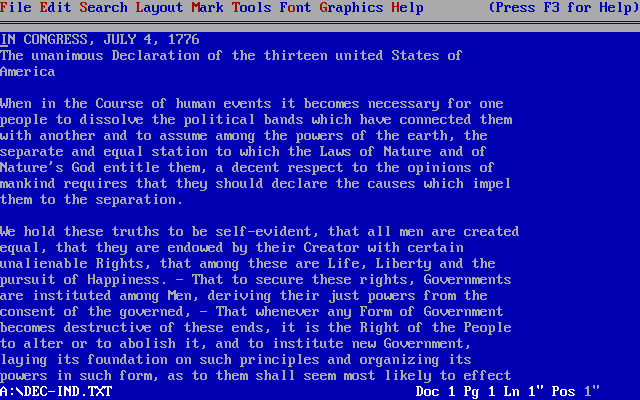
\includegraphics[width=12cm]{images/wordperfect.png}}
\caption{A screenshot of Wordperfect 5.1, running in Microsoft DOS circa 1989.}\label{figure:wordperfect}
\end{figure}

\begin{figure}

\begin{verbatim}
                \documentclass{article}
                \begin{document}
                \textbf{Hello world}
                \end{document}
\end{verbatim}
\center{(a)}
\begin{verbatim}
                <html>
                  <body>
                     <b>Hello world</b>
                  </body>
                </html>
\end{verbatim}
\center{(b)}

\caption{Examples of the words `hello world' in bold text typeset (a) \LaTeX\ and (b) HTML}\label{figure:helloworld}
\end{figure}


The huge advantage of WYSIWYG is that it's really easy to understand what's going on, and most people can create reasonably nicely formatted documents with relatively little effort. For short informal documents, one-off letters, memos and such, WYSIWYG works quite nicely. But if you've ever tried writing anything much longer, or that includes images and tables, you may have already started to see where the paradigm breaks down. For example, if you write ``Figure \ref{figure:menandcheeses} on page \pageref{figure:menandcheeses}  shows a picture of some men looking at cheese'', but then later on edit your document to include some more text at the start, and a new picture of a some broccoli (as in Figure \ref{figure:broccoli}), you'd have to search through your report to find all mentions of `Figure \ref{figure:menandcheeses}' and `page \pageref{figure:menandcheeses}' and manually update them to reflect the new numbering. This might be fine if you have two figures and five pages; but for a hundred-page report containing lots of pictures, you can see how this becomes tedious and error prone very quickly. 

\begin{figure}
\centerline{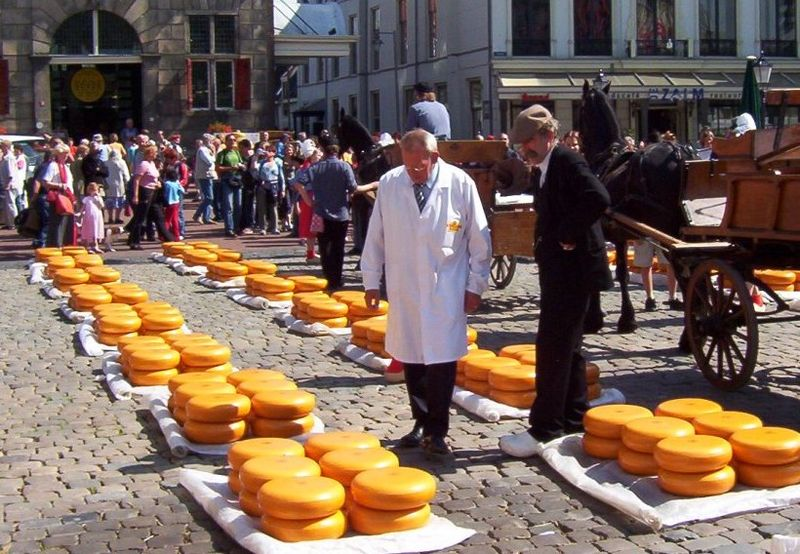
\includegraphics[width=10cm]{images/men-and-cheese.jpg}}
\caption{Some men, possibly Dutch, looking at cheeses.}\label{figure:menandcheeses}
\end{figure}

\begin{figure}
\centerline{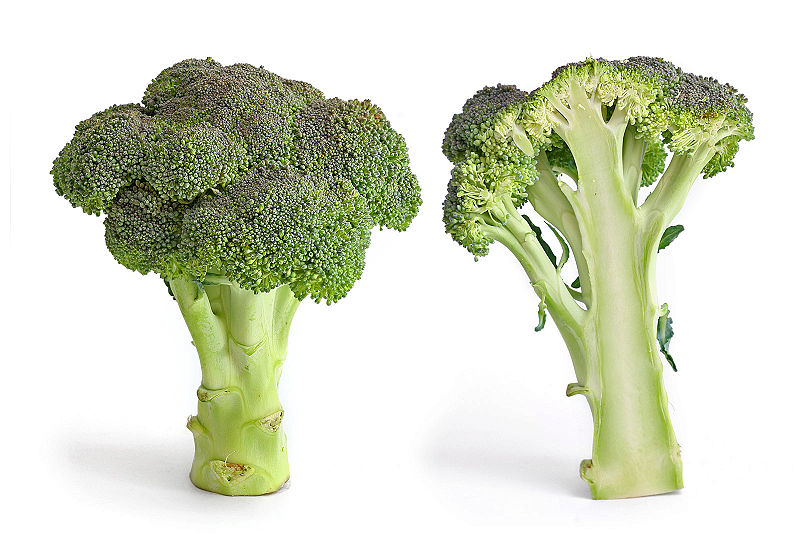
\includegraphics[width=10cm]{images/broccoli.jpg}}
\caption{Some broccoli.}\label{figure:broccoli}
\end{figure}

\section{Style and content}

The other thing about WYSIWYG is that it puts you entirely in control of the visual layout and style of your article, and this isn't necessarily a good thing for two reasons. First, it means that instead of focusing on the content and structure of what you're writing, it makes it easy to get distracted by tinkering with the layout and style. And although layout and style are of course important if you want to create a professional-looking document, they are definitely always secondary to content and structure. Second, it means that you are, well, entirely in control of the visual layout and style of your article. And although it might not be obvious up-front, such control is not necessarily a good thing unless you really know what you're doing (and unless you are a talented graphic designer with a deep understanding of typography, you almost certainly don't\footnote{Don't take this personally; we're in the same boat. If you think that this document is nicely formatted, that's all down to \LaTeX, not us!}). Creating documents that are aesthetically pleasing and easy to read is rather a specialist skill with its origins going all the way back to Caxton's invention of the printing press in the fifteenth century.  Over the years, typographers have honed their skills, arriving at complex rules and heuristics that determine the optimum number of characters on a line, ideal relative and absolute font sizes, spacings, margins, figure placement and so on that lead to attractive---and most importantly---readable documents. You could of course learn all these rules, and make sure you implement them manually using your favourite WYSIWG editor, but that's not what a Computer Science degree is about. The \LaTeX\ system implements many of these rules, making decisions for you about the best way to lay your document out on the page. This allows you to concentrate on creating good quality content, safe in the knowledge that \LaTeX\ will do a good job of presenting it out for you. The idea of separating out \concept{content} from \concept{presentation} is something you'll encounter many times during your studies of Computer Science. You'll see it again in a fairly obvious way soon when you come to writing some HTML and CSS in Phase 3 of this course unit: but the concept of distinguishing between a \concept{model} and a \concept{view} will reappear in increasingly subtle ways throughout your degree. 

\section{The right tool for the right job}

To avoid any  misunderstanding, we are not at all trying to claim that \LaTeX\ is `better' than Word (or similar), just that it's `different', in fact, `extremely different', both in its capabilties, and its conceptual model. One of the key skills that any professional needs to learn is to be able to choose the right tool for the right job. If you're going to open a coconut, you'll probably use a corkscrew, not a pneumatic drill. Similarly, if you're writing a quick letter, or making a DO NOT DISTURB sign, you'll probably want to use a quick WYSIWYG tool like Word. If, however, you're writing a technical document, perhaps with some maths, or a 3rd Year Project Report, or an article you want to get published, then you'll probably want \LaTeX.  You might see analogies with programming here---and which languages are best suited to which jobs.

\section{Getting started}

The downside of using a non-WYSIWYG system such as \LaTeX\ is that there is rather more to understand and master before you can get going. You will have probably spotted that this is a recurring pattern: to perform certain tasks, we often have the choice between two approaches: the first (in this case the WYSIWYG way) allows you to get going straight away as a novice, but doesn't allow us to grow much expertise to get better and faster, and as you try to do more complex things, you discover problems and limitations that are hard to overcome; the second is inherently more powerful, but requires you to invest time and effort before you can get started. Wordprocessors and file browsers fall into the former category; \LaTeX\ and use of the command line into the latter.

By the time you get to write your third year project report, you will almost certainly want to use \LaTeX. Indeed, that might well be the point at which you will gain the most benefit from it throughout your studies here. What you do not want is to be having to learn \LaTeX\ at that point--it will be challenging enough without that extra burden. So, we are embarking you on a programme of learning \LaTeX\ more gradually.

%Start by creating the directory $HOME/COMP10120/ex4 and make it your current one. 

\section{The exercises}


\exercisess{A closer look}
%\subsection{Exercise 1}
\label{sec:exercise-1}


Fire up your favourite editor, enter the following text (it's important that you enter it exactly as it is below for now), and then save it as a file called \fname{fire-and-ice.tex} (in case you're wondering, it's the first line from a short poem called `Fire and Ice' by American poet Robert Frost \citep{frost1923}; the whole poem is on the \href{http://www.poetryfoundation.org/poem/173527}{Poetry Foundation website} if you're interested.)

\begin{verbatim}
\documentclass[a4paper]{article}
\begin{document}
Some say the world will end in fire,
\end{document}
\end{verbatim}
%
Next, run the command \texttt{pdflatex fire-and-ice.tex} (for now it's sufficient to say that pdflatex invokes \LaTeX\ to create a PDF file as the output; the full story is a bit more complicated.)

\LaTeX\ will process your file, and print out a surprisingly large amount of text into the shell window as it does so. If all is well, the last two lines printed out will be something like:

\begin{verbatim}
Output written on fire-and-ice.pdf (1 page, 11853 bytes).
Transcript written on fire-and-ice.log.
\end{verbatim}
%
after which \LaTeX\ will return you to the command prompt. If you've made a mistake typing in the file, \LaTeX\ will stop part way through processing your work, and display an error (possibly, quite an obscure one) and show a `?' prompt. The best thing to do at this stage is to press \ctrl{d}, or \ttout{x}, to tell \LaTeX\ to give up trying to process your file. Then fix the mistake, and try again.  

If you now list the contents of the directory, you should see that a file called \fname{fire-and-ice.pdf} has been created (along with two other files called \fname{fire-and-ice.aux} and \fname{fire-and-ice.log} both of which we will ignore for now). Use one of the PDF readers (such as \cmdname{evince}) to look at the content of \fname{fire-and-ice.pdf}.  Admittedly, it's not the most exciting result; if everything has worked properly so far, you should see single-page document with the words `Some say the world will end in fire,' a little way down from the top of the page\footnote{If you have been carried away with the sheer excitement and joy of learning to use \LaTeX\, and improvised the text rather than typing the first line of `Fire and Ice' as requested, please go back and change it now: it really is important that you use exactly that text. Really, it is. That's better. Thanks.}.

But now look more closely. A lot more closely\ldots really zoom in. See anything interesting?

Even for this very short document, \LaTeX\ has taken a fairly sophisticated typographical decision on your behalf and \concept{ligated} (which is typo\-graphy-speak for `joined') the `f' and the `i' in the word `fire'; the spacing between the characters has been subtly altered so that the dot above the `i' and the blob on the end of the curvy bit (the `arc of the stem', if we're being formal) on the top of the `f' join together to form a single shape called a \concept{ligature}. Why? Because having two blobs side by side simply looks a bit clumsy as you can see in Figure \ref{figure:twofires}. To make this decision, \LaTeX\ has had to know a lot about the fonts being used (not all `f's in all fonts have a blobby end; not all `i's in all fonts have a round dot that would merge nicely with the blobby bit on the end of an `f', and so on). There's a reasonable chance that you've never heard of ligated characters before---it is, after all, a fairly specialist thing. And there are hundreds of other obscure but important `rules' of typography that go to make professionally typeset documents look good\footnote{Look up `kerning', `combining characters' and `serif' on Wikipedia for starters. And if you're really keen, Donald Knuth's fascinating and compendious book `Digital Typography' \citep{knuth1999} has an entire chapter dedicated to the joys of the letter `S'. Probably best not to bring this subject up at the pub though, or at parties. Unless they are very specialist parties.}. Individually, they might not be obvious or hugely important, but collectively and subliminally they make the difference between something that looks just-about-acceptable (like most things written using wordprocessors) and things that stand out as looking really professional (you might want to remember this when it comes to putting your CV together.)

\begin{figure}[htbp]
\centerline{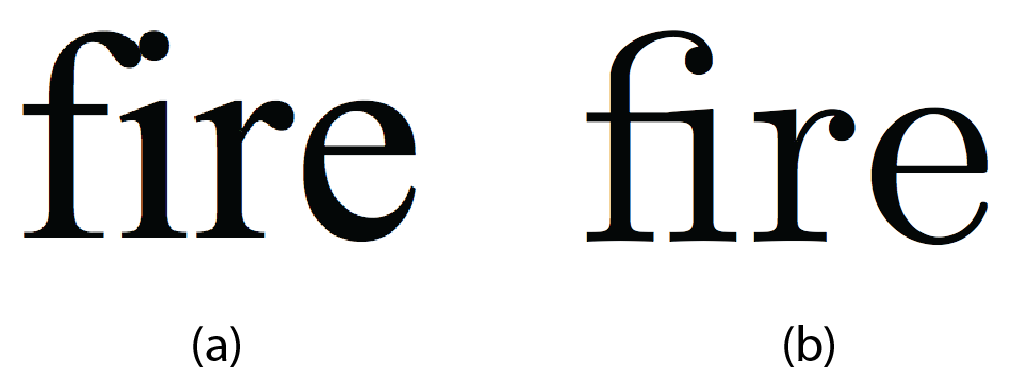
\includegraphics[width=6cm]{images/fireandfire.png}}
\caption{The word `fire' typeset by (a) Microsoft Word 2011 without ligated characters, and (b) by \LaTeX\ showing the ligation of the characters `f' and `i'.}\label{figure:twofires}
\end{figure}
%
But that's enough about the typography of the word `fire' for now. Let's put together something more substantial. 

\exercisess{A larger example}
%\subsection{Exercise 2}
\label{sec:exercise-2}

 Create yourself a new file, called \fname{sections.tex} by copying \fname{fire-and-ice.tex}. In \fname{sections.tex}, replace the line of poetry with the text from Figure \ref{figure:bleakhouse} (which contains the first three paragraphs of Dickens' novel, `Bleak House' \citep{dickens1852}).

\begin{figure}[tbp]

\begin{quote}

  \itshape
  \raggedright
  
London. Michaelmas term lately over, and the Lord Chancellor sitting
in Lincoln's Inn Hall. Implacable November weather. As much mud in
the streets as if the waters had but newly retired from the face of
the earth, and it would not be wonderful to meet a Megalosaurus,
forty feet long or so, waddling like an elephantine lizard up Holborn
Hill. Smoke lowering down from chimney-pots, making a soft black
drizzle, with flakes of soot in it as big as full-grown
snowflakes--gone into mourning, one might imagine, for the death of
the sun. Dogs, undistinguishable in mire. Horses, scarcely better;
splashed to their very blinkers. Foot passengers, jostling one
another's umbrellas in a general infection of ill temper, and losing
their foot-hold at street-corners, where tens of thousands of other
foot passengers have been slipping and sliding since the day broke
(if this day ever broke), adding new deposits to the crust upon crust
of mud, sticking at those points tenaciously to the pavement, and
accumulating at compound interest.



Fog everywhere. Fog up the river, where it flows among green aits and
meadows; fog down the river, where it rolls defiled among the tiers
of shipping and the waterside pollutions of a great (and dirty) city.
Fog on the Essex marshes, fog on the Kentish heights. Fog creeping
into the cabooses of collier-brigs; fog lying out on the yards and
hovering in the rigging of great ships; fog drooping on the gunwales
of barges and small boats. Fog in the eyes and throats of ancient
Greenwich pensioners, wheezing by the firesides of their wards; fog
in the stem and bowl of the afternoon pipe of the wrathful skipper,
down in his close cabin; fog cruelly pinching the toes and fingers of
his shivering little 'prentice boy on deck. Chance people on the
bridges peeping over the parapets into a nether sky of fog, with fog
all round them, as if they were up in a balloon and hanging in the
misty clouds.

Gas looming through the fog in divers places in the streets, much as
the sun may, from the spongey fields, be seen to loom by husbandman
and ploughboy. Most of the shops lighted two hours before their
time---as the gas seems to know, for it has a haggard and unwilling
look.

\end{quote}

\caption{Some sample text from the opening of the Dickens' novel `Bleak House' \citep{dickens1852}.}\label{figure:bleakhouse}
\end{figure}

Edit the text to make sure that there is a blank line between each of the three paragraphs (it's not enough that each paragraph starts on a new line of its own, there has to be an empty line in between them). That's how paragraphs are distinguished in \LaTeX\ (in fact, it doesn't matter how many blank lines you put as long as there is at least one\ldots for the most part \LaTeX\ ignores spare whitespace). Now type a paragraph of gibberish by randomly hitting keys on the keyboard, and putting spaces in to make `words' in the text file. You should end up with something like the following, but about three times as long (don't cut and paste this from here\ldots it's important that you actually create some unique gibberish yourself!):

\begin{verbatim}
Oisjdf oqweqwe oi soijs hbweo kbsd oijsdf 
oijqwknpiouh iusbdfspb sifuhygwqeb usgweijf 
blimqwoq oieuerwefwiu aokqjw uioshiufds 
qiqks odfubfi psdiweneq.
\end{verbatim}

Be careful at this stage to only include letters (uppercase and lowercase), commas, full-stops and perhaps numbers in your gibberish text: if you use any other symbols, you may upset \LaTeX. 

Next go to the website \href{http://www.lipsum.com/}{http://www.lipsum.com} and follow the instructions to generate yourself three paragraphs of what's called \concept{Lorem Ipsum} text. Copy and paste that text into your \LaTeX\ document too (don't worry about what it means at this stage), again making sure that you have a blank line between the paragraphs.

Re-run \texttt{pdflatex} and look at the resulting \fname{sections.pdf}. Again, at first glance, there's nothing hugely exciting going on here: the text from your \fname{.tex} file has been assembled into a (probably) two page PDF document. But in fact quite a few things have happened: 

% \begin{note}
%   Why don't we indent pars? Because we have lots of short ones?
% \end{note}

\begin{itemize}
\item The blank lines that separate the paragraphs in your source file are gone, and instead \LaTeX\ has indented the first line of each paragraph. There's nothing profound here about the decision to indent paragraphs rather than (say) to leave a gap between them (so called \concept{block paragraphs}); it's just \LaTeX's default paragraph style, and can be changed easily enough.\footnote{Though apparently, there is some evidence in \cite{tinker63} that indented paragraphs increase readability}
\item There are page numbers at the bottom of each page. This is a very sensible default, allowing you in meetings to ask people to ``turn to page 4'' and so on (it's a bit odd, and a source of some annoyance, that most wordprocessors don't do this by default too). But you can easily switch page numbers off, change their style or move them elsewhere if you need to. 
\item The text is \concept{fully justified} so that it's flush on both the left and right hand edges.
\item Certain words that fall at the end of lines have been hyphenated, even if they weren't originally split by hyphens in the source text.
\end{itemize}

These last two points about justification and hyphenation might seem utterly trivial, but getting these factors right turns out to be an important part of making readable documents; readability is not just about which font you choose, but about how the characters and spaces are distributed on each line. It's something that you will have seen happen so often in professionally typeset materials that you'll have taken it for granted, and you may not have spotted that it doesn't happen in quite the same way when you use a wordprocessor. The principle behind justifying text seems easy enough at first glance: you simply have to take any `left over' space that would be at the end of a line, and redistribute it between the words in some way to `space them out' a bit more so that they take up all the available horizontal room. But it turns out to be much harder than it seems, and all the simple ways you might think of for doing this on a per-line basis give results that are visually quite unsatisfactory, with nasty patterns made up of neighbouring whitespace appearing in the layout and ruining everything. The added complication here is that to do the optimum job of shuffling the words round on their lines, you really need the flexibility of being able to hyphenate words to give you extra space on lines that would otherwise be tightly packed with characters. But if you hyphenate words badly, by breaking them in inappropriate places, or do it too often then that makes the text hard to read too. It's all deeply inconvenient and inter-related. The best solution to this aesthetic conundrum so far was developed by \cite{SPE:SPE4380111102} and later improved by Frank Liang during his PhD research \citep{liang}, and it's a technique that tries to optimise the layout of whole paragraphs rather than individual lines. The algorithm takes into account all manner of different things: language-specific character patterns, the number of consecutive lines that end with hyphens, the word `tightness' on each line\ldots any many others. The details don't really matter here, but the really important thing insight is that you get better results by working on a bigger chunk of the document (in this case a paragraph at a time) rather than trying to independently optimise lots of small bits (say, lines) and hoping that the result of joining them all together turns out nicely. This idea of optimising things \concept{globally} versus \concept{locally} is something you'll see many times throughout your Computer Science degree; watch out for it in all the algorithms courses.

This highlights a fundamental difference between the WYSIWYG para\-digm and the way that documents are produced using \LaTeX. As we've seen, small changes down at the the level of individual characters can have fairly large knock-on consequences for the optimal layout of a document: changing one letter for another affects the length of a line, which in turn affects the hyphenation options, which then affects the length of a paragraph, which means that the best place for a figure that was on page 99 might now on page 100, but that means that all references to `page 99' now need a bit more room to account for the extra digit which means that the some line lengths have changed which means\ldots well, you get the idea. It's more complicated that it first seems. \LaTeX\ gets to see the \emph{whole of your document at once}, and can therefore make decisions about how best to hyphenate lines,  position figures or whatever else it likes \emph{before} it shows you the results; so it can make solutions that are optimal for the whole document, as well as looking at details such as ligated characters. Wordprocessors can't afford to do this since it would be deeply distracting if every time you typed a character, the whole layout of the document flapped around in front of your eyes. Wordprocessors can only sensibly make little optimisations at a local (probably per-line level). It's not that wordprocessors are rubbish, or that the people that programmed them were lazy: it's a fundamentally different way of working, and knowing the pros and cons of the different approaches will help you pick the right tool for the job. 

You may have noticed that actual text in your document (and in fact, this one) takes up a (perhaps) surprisingly narrow horizontal region of the page. This last `feature' might seem odd at first, but it illustrates another important typographical point that you may never have thought of before: reading long lines of text is hard, because your eyes find it hard to move in a completely straight line as they scan from left to right. So the longer the line of words, the more you have to work to keep your eyes from accidentally drifting up or down onto a neighbouring line (perhaps you've experienced the phenomenon of accidentally re-reading the same line over and over as your eyes get tired). It may never have occurred to you, but most books have relatively short lines of text; and those that use large pages often split text into several columns so that individual lines are kept relatively short. The widely trusted book `The Elements of Typographic Style' \citep{bringhurst92} makes the following assertion:

\begin{quote}
\emph{
``Anything from 45 to 75 characters is widely-regarded as a satisfactory length of line for a single-column page set in a serifed text face in a text size. The 66-character line (counting both letters and spaces) is widely regarded as ideal.''}
\end{quote}

\LaTeX\ knows about this issue, so made a sensible default decision for you. You may have noticed that there is a subtle difference in appearance of this chapter from previous ones: the lines are shorter and paragraphs are indented. We wanted to use the default \LaTeX\ layout for this chapter, but changed it for earlier chapters in an effort to save paper.

There's one last unusual thing to note: your paragraph of gibberish text in between the real words from Bleak House and the \concept{Lorem Ipsum} almost certainly stands out and looks really quite odd (it might even have confused \LaTeX's hyphenation rules enough to have ended up with one or more lines sticking out proud of the right hand margin).  Let your eyes relax so that your vision blurs for a moment: you can still probably spot that the gibberish paragraph looks out of place. It's quite likely that you even found creating the gibberish unexpectedly hard. The interesting thing here is that as humans, we spend so much time reading and writing `proper' natural language that we become attuned to the patterns of letters words and the underlying `rhythm' of our written language that its very hard to artificially reproduce something that looks plausible; the frequency of the letters you chose by randomly hitting keys, and the length and patterns of the words you put in place most likely don't match the natural patterns of real languages, so they just look plain wrong.  Curiously the \concept{Lorem Ipsum} text that you got from the website probably doesn't look so bad, in spite of it not being made up of real words. But that's not surprising since \concept{Lorem Ipsum} is specifically created to be used as a placeholder for real text when typesetting. While the words are meaningless Latin-like things, their length, and the distribution of characters and word lengths are chosen to mimic patterns in real language.

% \exercisess{Creating document structure}
% %  \subsection{Exercise 3}
% \label{sec:exercise-3}

Next let's give our document some structure by dividing it up into sections. On the line before Bleak House starts, add the command

\begin{verbatim}
\section{Bleak House}
\end{verbatim}
%
making sure it appears on a line of its own. Then just before your paragraph of gibberish, put similar a similar instruction (again, on its own line), and then create a final section before the Lorem Ipsum. Rerun pdflatex and look at the results. You should see the section headings appear in the appropriate places in the PDF, automatically having been given section numbers. Experiment by adding in a couple of sub-sections towards the end of the document using the  \verb|\subsection| command, which like \verb|\section| command above takes as a parameter some text in contained in wiggly brackets. 

Now, at the top of your document after the \verb|\begin{document}| line and before the command defining the first section, add the following two commands, each on their own line:

\begin{verbatim}
\tableofcontents
\newpage
\end{verbatim}
%
  Re-run pdflatex \emph{twice}, and check that the effect is what you'd expect. You need to process the source twice because on the first run, \LaTeX\ gathers and stores information about what to put in the table of contents, and only creates it on the second run.


\section{Common formatting features}

Before we give you some more exercises to do, here is a brief introduction to some commonly used features of \LaTeX.

\subsection{Enumerated and bulleted lists}

Creating bulleted or numbered lists in \LaTeX\ is straightforward, and is done like this:

\begin{verbatim}
\begin{enumerate}
\item My first item
\item My second item
\item The last thing on my list
\end{enumerate}
\end{verbatim}
%
You must make sure that you both \texttt{begin} and \texttt{end} your list, and that each item is terminated by a newline. Changing `enumerate' to `itemize' gives you a bulleted rather than numbered list (note the American spelling of `itemize').  

\subsection{Bold and italic text}
Text can be typeset in \textbf{bold} font using the \verb|\textbf|, and \textit{italics} using \verb|\textit| as in the example below:

\begin{verbatim}
Some say the \textbf{world} will end in \textit{fire},
\end{verbatim}

\subsection{Cross referencing}

\LaTeX\ allows you to cross-reference almost anything in the document, which includes sections, sub sections and figures. To use the cross-referencing feature you simply insert the command 
\begin{verbatim}
\label{mymarker}
\end{verbatim}
at the point in the document you want to refer to, and then use the command

\begin{verbatim}
\ref{mymarker}
\end{verbatim}
when you want to use the reference. Obviously you replace the text `mymarker' with something more meaningful. An important tip here is to call the marker something that refers to the content of that part of the document, and to avoid the temptation to use numbers (so don't call your marker `section1', instead call it `introduction'; if you reorder your document, it's still likely to be the introduction, but it may no longer be Section 1). For example:

\begin{verbatim}
\section{Reflection on Welcome Week}
\label{welcomeweek}
I spent most of welcome week getting to know my way
around campus. I should have made more effort to join
societies I think; I must remember to get to the
Students' Union and take a look around there.

\subsection{Things I enjoyed}
Everything so far has been wonderful, with the caveat I 
mentioned in Section \ref{welcomeweek}.

\subsection{Things I didn't enjoy}
I've discovered that I don't like soggy chips.
\end{verbatim}

The really useful thing about cross-referencing in \LaTeX\ is that you'll get warnings when you compile your document if cross-references are undefined or used incorrectly. This means you don't have to manually check every reference in your document to make sure its still right. You do, however, have to run \LaTeX\ twice, for similar reasons to those given above.

\subsection{Figures and pictures}

Including figures and pictures in your document is easy. You do it like this:

\begin{verbatim}
\begin{figure}
\centerline{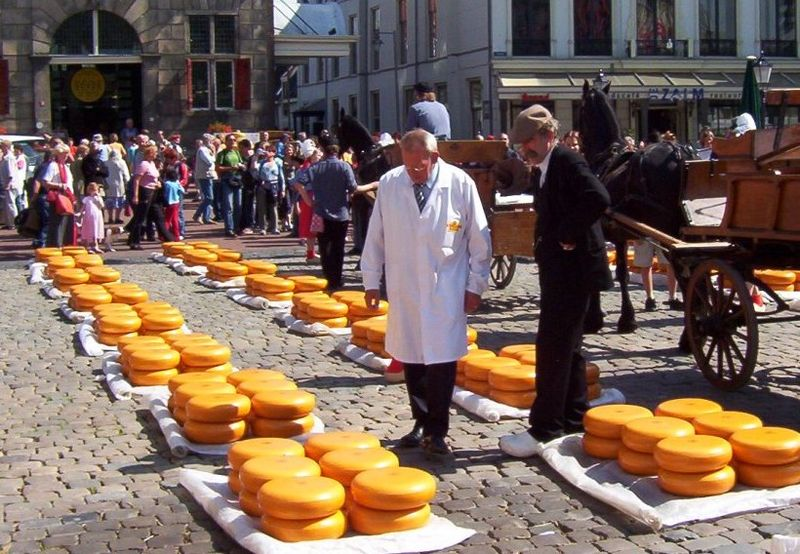
\includegraphics[width=10cm]{images/men-and-cheese.jpg}}
\caption{Some men, possibly Dutch, looking at cheeses.}
\label{figure:menandcheeses}
\end{figure}
\end{verbatim}
which we used to create Figure~\ref{figure:menandcheeses}. You can probably see what's happening. The command \verb|\includegraphics{}| gets your image, which can be PDF, PNG, JPG, GIF or PostScript. The \verb|\begin...\end| code `wraps' up whatever picture you're including, and allows \LaTeX\ to treat it as an unbreakable \concept{floating} thing that it will position for you as best it can in the document, while maintaining an overall nice typographical layout. This floating of figures can sometimes result in the figure ending up in a place you didn't expect, but in most cases \LaTeX\ will make the most sensible choice. It's possible to exercise finer control over figure placement, but that's beyond the scope of this exercise.

The \verb+\includegraphics+ command is not built in to core \LaTeX\ but is in an additional \emph{package}, which needs to be explicitly loaded. We load this package by this using the command \verb+\includepackage{graphicx}+ in the document preamble, i.e.\ after the \verb+\documentclass+ command, but before  \verb+\begin{document}+.


\exercisess{Including images}
Create a document \fname{image.tex}, that contains some text (maybe from 'Lorem Ipsum', together with a figure containing an image of your choice, perhaps the one you made in Intro Lab 2 like Steve's Mr Noodle. There should also be a reference to the figure in the text. You should first use the program \cmdname{convert} (check its man page) to create a \fname{PDF} version of the file.


\subsection{Typesetting Mathematics}
\label{mathssection}

Earlier we saw this formula:

\[ x = \frac{-b \pm \sqrt{b^2-4ac}}{2a} \]
It looks nice, doesn't it? To tell \LaTeX\ to display this, you have to type a bit of magic, but it's easily-learned magic. To create such a formula in a WYSIWYG editor, there is also magic involved, but it usually involves a lot of mouse-clicking, and remembering special key combinations like 'control-this' and 'alt-that'. In \LaTeX\ it doesn't. You simply type this:
\begin{verbatim}
     \[ x = \frac{-b \pm \sqrt{b^2-4ac}}{2a} \]
\end{verbatim}
You can probably work out how most of this creates the formula, but it won't be obvious that the \verb|\[| and  \verb|\]| characters that enclose the formula mean ``typeset this as a displayed formula, giving it some vertical space from the surrounding text''. If we'd used \verb|\(| and \verb|\)| instead to enclose the formula it would appear in-line, like this: \(  x = \frac{-b \pm \sqrt{b^2-4ac}}{2a} \). It still looks very nice, and observe how it's automatically been resized to fit, and that the lines of text have had their spacing changed a bit. This all looks simple, but the implementation inside \LaTeX\ and \TeX\ is complex. It involves parsing the description of the formula to create a corresponding tree data structure, which is then \concept{recursively walked}' to work out the horizontal and vertical typographical spacings needed. You'll meet these ideas in \courseunit{COMP11120} and \courseunit{COMP26120} Algorithms and Imperative Programming.

Here's another example, taken from \courseunit{COMP27112} Computer Graphics (it's a `simple' local illumination model incorporating ambient, diffuse and specular reflection by multiple lights):

\[ I = k_a I_a + \sum_{i=1}^M {\frac{{I_p}_i}{d'_i}} [ k_d(\hat{N}\cdot\hat{L_i}) + k_s(\hat{R_i}\cdot\hat{V})^n] \]
%
We write this in \LaTeX\ as follows:

\begin{verbatim}
    \[ I = k_a I_a + \sum_{i=1}^M { \frac{{I_p}_i}{d'_i} }
    [ k_d(\hat{N} \cdot \hat{L_i}) 
    + k_s(\hat{R_i} \cdot \hat{V})^n] \]
\end{verbatim}
%
Try to match the \LaTeX\ commands with the formula displayed above. You'll see lots of curly brackets, and this example illustrates their two uses in \LaTeX. The first is to provide an argument to a command; for example \verb|\hat{N}| means ``apply the \verb|\hat| command to $N$'', which creates \(\hat{N}\), the vector \( N \) with a little hat  on.  

The second use of curly brackets is to group things together to avoid ambiguities. In the example you can see \verb|\sum_{i=1}^M|, which creates a summation sign and its lower and upper limits: \( \sum_{i=1}^{M} \). We wrap the lower bound, \verb|i=1|, in curly brackets to group it into an indivisible unit. If we were to omit the brackets, writing \verb|\sum_i=1^M|, \LaTeX\ would then produce \( \sum_i=1^M \), which is not at all what we want (even \LaTeX\ can't always know what we really want).

One final example. If we tell \LaTeX:

\begin{verbatim}
   \[ T_1 = \left[
    \begin{array}{cccc}
    \cos \theta & -\sin \theta & 0 & \delta \\
    \sin \theta  & \cos \theta & 0 & \epsilon \\
    0 & 0 & 1 & \eta \\
    \alpha & \beta & \gamma & 1
    \end{array}
    \right] \]
\end{verbatim}
%
we'll get a splendid matrix which expresses a particular 3D geometrical transformation (don't worry if you don't recognise this, you'll be introduced to matrix notation in the latter part of \courseunit{COMP11120}: Mathematical Techniques for Computer Science. For now you can just treat it as some mysterious maths):

\[   T_1 = \left[
    \begin{array}{cccc}
    \cos \theta & -\sin \theta & 0 & \delta \\
    \sin \theta  & \cos \theta & 0 & \epsilon \\
    0 & 0 & 1 & \eta \\
    \alpha & \beta & \gamma & 1
    \end{array}
    \right]
\]
%

In the \LaTeX\ code,  \verb|\left[| means ``big opening square bracket please'';  \verb|{cccc}| means ``an array with 4 columns please, with the items in each column centred"; \verb|&| means ``start a new column''; and \verb|\\| means ``start a new row''. You'll notice that \LaTeX\ knows about  greek letters; it knows about all standard maths symbols too, and also they ways  they're usually used.


\subsubsection{A longer piece of mathematics}
\label{sec:longer-piece-maths}

  We conclude this section with an example of a longer piece of mathematics, that shows how you might typeset a complete mathematical argument rather than a single formula. The example is Euclid's proof of the fact that $\sqrt{2}$ is irrational. It's an argument that has been covered in COMP11120 and is an example of proof by contradiction. It starts by making the assumption that it is \emph{not the case} that $\sqrt{2}$ is irrational, in other words that we can find integers $p$ and $q$ with $\sqrt{2} = p/q$.

  We can assume, without losing anything, that $p$ and $q$ have \emph{no common factors} (Why?)
  \[
  \begin{array}{lcl}
     \sqrt{2}    & = & p/q \\ 
      q\sqrt{2} & = & p   \\ 
      2q^2       & = & p^2 \\ 
  \end{array}
  \]
  This means that $p^2$ is even, from which we can also deduce that $p$ is even. (Why?)

  This means that $p = 2k$, for some $k$, so \ldots
  \[
  \begin{array}{llcl}
                       & 2q^2 & = & (2k)^2 \\ 
      \therefore & 2q^2 & = & 4k^2   \\ 
      \text{so}   & q^2   & = & 2k^2   \\
   \end{array}
  \]
  But this means that $q^2$, and hence $q$ is  even. Since $p$ and $q$ are both even we have a contradiction to our initial assumption, so no such $p$ and $q$ exist.

The way this is formatted is shown here:

{\small
\begin{verbatim}
 We conclude this section with an example of a longer piece of mathematics,
that shows how you might typeset a complete mathematical argument rather
than a single formula. The example is Euclid's proof of the fact that
$\sqrt{2}$ is irrational. It's an argument that has been covered in
COMP11120 and is an example of proof by contradiction. It starts by
making the assumption that it is \emph{not the case}that $\sqrt{2}$
is irrational, in other words that we can find integers
$p$ and $q$ with $\sqrt{2} = p/q$.

  We can assume, without losing anything, that $p$ and $q$ have
 \emph{no common factors} (Why?)
  \[
  \begin{array}{lcl}
     \sqrt{2}   & = & p/q \\ 
      q\sqrt{2} & = & p   \\ 
      2q^2      & = & p^2 \\ 
  \end{array}
  \]
  This means that $p^2$ is even, from which we can also deduce that $p$
is even. (Why?)

  This means that $p = 2k$, for some $k$, so \ldots
  \[
  \begin{array}{llcl}
                 & 2q^2 & = & (2k)^2 \\ 
      \therefore & 2q^2 & = & 4k^2   \\ 
      \text{so}  & q^2  & = & 2k^2   \\
   \end{array}
  \]
  But this means that $q^2$, and hence $q$ is  even. Since $p$ and $q$ are
 both even we have a contradiction to our initial assumption, so no
 such $p$ and $q$ exist.
\end{verbatim}
}

  \LaTeX\ really shines at typesetting mathematics, and it would take pages and pages to describe all the features. Have a look at:
\\
\\
\href{http://en.wikibooks.org/wiki/LaTeX/Mathematics}{http://en.wikibooks.org/wiki/LaTeX/Mathematics}
\\
\\
for a flavour. 
 
\section{More Exercises}

\exercisess{A reflection on your studies}
Your first \LaTeX\ document will be a very brief reflection on your studies so far.

You should work in \verb+$HOME/COMP10120/ex3+. Write a hand-crafted \LaTeX\ document called 
\fname{courses-reflection.tex} (exact name please, otherwise submit will not work). It will have the following structure.

\begin{enumerate}
\item 
Appropriate title including author and date.
\item Table of contents.
\item A brief paragraph saying what the document is about.
\item  A section, appropriately titled, for one of your courses, containing:
  \begin{itemize}
  \item  a brief paragraph saying what the course is about. This will contain a citation referring to the URL of the course syllabus page.
 \item A sub-section, appropriately titled, containing an enumeration of the three things you like the most about the course.
\item A sub-section, appropriately titled, containing an enumeration of the three things you like the least about the course.

  \end{itemize}
 A repeat of item 4 for each other course you are studying. These sections should appear in alphabetical order by course code (e.g. COMP10120).
\end{enumerate} 
After completing and successfully compiling and viewing your document, you should spell-check it as follows.

\begin{ttoutenv}
ispell courses-reflection.tex   
\end{ttoutenv}

Once you are completely satisfied with it, produce a hard copy ready for marking.

% \exercisess{Arguments about software patents}
% \label{sec:exercise-2:-arguments}

% \begin{note}
%   This won't work and needs replacing
% \end{note}

% In this exercise you will create three documents which have two shared parts in common. All together you will create five files as follows (please be exact with the filenames).

% pros-and-cons.tex This will be a document that contains the pros and cons of software patents. It will contain a paragraph explaining what the document is about, a section listing the pros, another section listing the cons and finally a section concluding the balanced argument.
% for.tex This will be a document that contains only the pros of software patents. It will contain a paragraph explaining what the document is about, a section listing the pros and finally a section concluding the argument for software patents.
% against.tex This will be a document that contains only the cons of software patents. It will contain a paragraph explaining what the document is about, a section listing the cons and finally a section concluding the argument against software patents.
% pros.tex This will be a piece of \LaTeX\ (not a full document) that will be included in the first and second document.
% cons.tex This will be a piece of \LaTeX\ (not a full document) that will be included in the first and third document.
% Just to be clear, you will not cut and paste the pros and cons lists into the two documents they each finally appear in. Instead you will arrange for the file containing each list to be input by the two documents. The idea here is that if you think of more pros or cons, or wish to change the wording of any, you can edit the corresponding single file, and the changes will appear in both documents that use it. You will need to find out how to make a \LaTeX\ source file input another one.

\exercisess{Formatting mathematics}
\label{sec:exercise-maths}

 Now for an exercise that involves some mathematics. Please create a file \fname{f-w.tex} which typesets the following piece of text and mathematics.
\begin{quote}
  % \documentclass{article}
% \usepackage{palatino}

% \begin{document}
There are many positive integer solutions to the equation
\[
x^2 + y^2 =  z^2
\]
which can be rewritten as
\[
z = \sqrt{x^2 + y^2}
\]
For example \((3,4, 5)\) or \((5,12,13)\). Such solutions are called \emph{Pythagorean triples}.

However, for higher powers the situation is very different, and we have:-

\noindent \textbf{Theorem: Fermat-Wiles}\\
For all natural numbers \(n \ge 3 \), there are no integers $x, y, z$ satisfying the equation
\[
x^n + y^n = z^n
\]
% \end{document}

\end{quote}

% \begin{center}
%   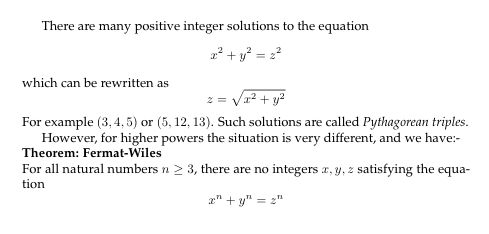
\includegraphics[width=.95\textwidth]{images/f-w}
% \end{center}


\exercisess{Exploring more \LaTeX\ features (optional, but easy)} 

This exercise reinforces some of the things you've done already, but
also introduces some features of \LaTeX\ that will be new to you. Take
a copy of the file
\fname{/opt/info/courses/COMP10120/ex3/latex-intro.tex} and follow the
instructions it contains. You should read it \emph{before} you process
it with \LaTeX.

\exercisess{A neat directory listing (optional, harder)} 
The fact that \LaTeX\ source files are just text makes it easy to have them generated by a program. You are going to exploit this and use \LaTeX\ to produce a neat document containing a listing of the files in any directory.

Find how to create tables in \LaTeX\ tables using the tabular
environment.  Make a \LaTeX\ document by hand that uses a table to
neatly show the information about the files in some (small) directory
(as produced by \ttout{ls -l}).  Write a shell script, called
\fname{neat-ls}, that takes an argument which is the path name of a
directory, and produces a \LaTeX\ document containing the above table
for the given directory. The script could also process the \LaTeX\ and
display the resulting \fname{pdf} file.  Finally, find out about the \fname{longtable}
package and change your script to use that instead.

\exercisess{A cleaning rota (optional, even harder)}
Now you will write a shell script, called \fname{make-rota}, that generates a house cleaning rota. (Very handy for next year ...). This is a table with columns such as Kitchen, Bathroom and Lounge. The rows will be weeks in the year, labelled with a date (e.g. always a Sunday). The idea is that house mates can write their initials in the boxes, promising to clean the corresponding room in that particular week. Start by making a sample table by hand.

Your script should take a single argument which is the date of the first day of the first row, e.g.10/20/13 (the US format for 20 Oct 13). The result will be a document that contains as many rows as fit on a single page (find out by experimenting).

The dates of each row should be generated from the first. See the manual page for date to figure out how you can generate a date that is a number of weeks and days later than an existing one.


\subsection{Marking Scheme}

You can view a copy of the marking scheme used by \texttt{labprint} at\\
{\small \urlnop{studentnet.cs.manchester.ac.uk/ugt/labprint/readms.php?unit=COMP10120\&ex=ex3.xml}}


\section{Next steps}

\LaTeX\ is a very powerful tool, and it does take a little getting used to. But it's not as scary as it might initially seem, and you should find that it doesn't take long to learn the common commands and techniques to make your documents well-structured and readable. As you become more comfortable with the basics and understand the principles of typesetting, finding out how to do more complex and sophisticated things is easy---there are hundreds of tutorials on the web. 

Don't get carried away though, and use the features judiciously: just because you've found a cool new command doesn't mean that you should use it just to show off your \LaTeX\ skills: content and structure always trumps typographic twiddlings\footnote{For example, footnotes like this are, for some reason, a really tempting feature to use in \LaTeX, and in this document we have abused them mercilessly to illustrate a point. Footnotes were originally a means for mechanical typesetters to insert comments, corrections or additions to existing documents without having to adjust the layout of a whole page, and of course in digital typography this is no longer necessary. They can justifiably be used for citations (though it's not common to do so these days) and URLs if you don't want these intruding into the body of your text. And in some very very rare cases, they can be used as an aside to the main flow of the text (which is what has been done in this document). But this should be used sparingly\ldots. If something is important to say, put it in the main body of your text. If it's not, then perhaps you should think about leaving it out completely, or find some other way of including it. Asking the reader to look down at the bottom of a page to find out whether something is important or not is irritating, and as you've probably found out already, often means you lose track of your reading position. They also give the impression that the author isn't clear about whether something is important or not, which is never good. And long footnotes like this one---while \LaTeX\ will typeset them perfectly well---are just plain silly. Best avoid.}.

\section{Acknowledgements}

 The images in Figure \ref{figure:knuthlamport} are from Wikimedia Commons, via the wikipedia articles on Knuth and Lamport, and are in the public domain. Figure \ref{figure:wordperfect} is from Wikimedia Commons, via the wikipedia article on \href{http://en.wikipedia.org/wiki/WordPerfect}{WordPerfect}, and is in the public domain. Likewise, for Figure \ref{figure:menandcheeses} from the Wikipedia article on \href{http://en.wikipedia.org/wiki/Cheese}{cheese}. Figure \ref{figure:broccoli}, also via Wikimedia Commons, is reproduced with the permission of its creator \href{http://commons.wikimedia.org/wiki/User:Fir0002}{\emph{Fir0002/Flagstaffotos}} under the terms of the \href{http://commons.wikimedia.org/wiki/Commons:GNU_Free_Documentation_License_1.2}{GNU Free Documentation License}. Figure \ref{figure:movabletype} is a combination of images by Daniel Ullrich and Willi Heidelbach, both from wikipedia and both released under the GNU Free Documentation License.

\printbibliography[heading=subbibliography]
\end{refsection}

\restoregeometry
\setlength{\parskip}{4pt plus 1pt}%
\setlength{\parindent}{0pt}

\endinput

\section{License}

The text of this exercise is licensed under the terms of the \href{http://creativecommons.org/licenses/by/3.0/}{Creative Commons Attribution 2.0 Generic (CC BY 3.0) License}. 

\bibliographystyle{natbib}
\bibliography{latex-exercise}

\appendix

\section{Fire And Ice}
\label{appendix:fireandice}

\begin{quote}
Fire and Ice, \emph{by Robert Frost.}\\

\begin{verse}
Some say the world will end in fire,\\
Some say in ice.\\
From what I've tasted of desire\\
I hold with those who favor fire.\\
But if it had to perish twice,\\
I think I know enough of hate\\
To say that for destruction ice\\
Is also great\\
And would suffice.\\
\end{verse}
\end{quote}

\section{Search Terms}
\label{appendix:searchterms}

dots per inch  / resolution
contrast
LED / LCD / CRT / e-ink
emissive versus reflective
anti aliasing
reading in light / dark environments
annotating / doodling
viewing angles
brightness
levels of colour

use google / google scholar / ACM digital library



Kindle / iPad / eInk / retina display


\end{document} 

Any text, like this, that is after the end of the document is ignored. This can be a
handy place to keep general comments and/or old fragments of the document
which you want to keep.


\chapter{More Linux stuff: DRAFT VERSION}

\notesurl{desktop5}

\begin{note}
  This is where the script for the last exercise before reading week goes

\end{note}


\chapter{Appendix}

\notesurl{appendix}


\section{Directories in the Pi's root filesystem}
\label{appendix:pidirs}

\begin{table}
\begin{tabular}{lp{12cm}}
\hline
Directory & Description\\
\hline
boot & Contains the Linux kernel and other low-level packages needed to get the Pi to boot.\\
& \\
bin & Contains the binary executables for basic commands such as \totype{ls} and \totype{pwd}.\\
& \\
dev & This is a virtual directory that represents devices connected to the Pi as though they were files that you can read from and write to. \\
 & \\
etc & Contains configuration files used by various programs, and also the names and encrypted passwords of users\\
 & \\
home & Each user gets their own subdirectory of \fname{home}. \\
 &\\
lib & This is where \textit{libraries} are stored; these are bits of code that are shared between several programs.\\
 & \\
lost+found & If something bad happens and the system crashes half way through doing something, it will put a copy of files that it knows are in a broken state here.\\
media & When you mount removable storage devices such as USB memory stickets, they will appear as filesystems here.\\
 & \\
mnt & This directory is used to mount storage devices. \\
& \\
opt & When you install optional software that's not considered part of the operating system, it usually ends up here.\\
& \\
proc & Like dev, this is a virtual directory. This one contains accounting information about the various processes that are running on your Pi.\\
& \\
selinux & Contains utility files relating to Security Enhance Linux.\\
& \\
sbin & This contains special executable binary files associated with system maintenance.\\
& \\
sys & Various files needed by the operating system.\\
& \\
tmp & Many programs need to create temporary files as part of their execution; they go here, and get deleted when the system reboots.\\
& \\
usr & User-accessible programs and bits of configuration.\\
& \\
var & Another virtual directory, used by programs to store variables.\\
\hline
\end{tabular}
\caption{Standard Linux system directories.}\label{table-dirs}
\end{table}

\section{A Map Of Colossal Cave}
\label{appendix:colossal-map}
\includegraphics[width=13cm]{images/ColossalCaveAdventureMap}\\
\\
This map of Colossal Cave is reproduced here by kind permission of its author, Mari Michaelis. This is the `spoilers' version of the map, and contains clues as to how to solve the various puzzles in the game. If you want to play the game for real, you probably should make your own map, or at least use the spoiler-free version of the map available at \url{www.spitenet.com/cave}.

\section{Basic HTML}
\label{appendix:simplehtml}

\wikipedia{HTML}{HTML} is a markup language used for creating web pages. It
encodes the structure and content of a page, and it's interpreted by a
web browser in order to display the page. This section gives a very
quick overview of a few basic HTML features, and omits a lot of stuff,
most notably \wikipedia{CSS}{CSS} which is used to style the visual
appearance of the content encoded by HTML. You'll meet CSS properly,
later in the course.

For a complete HMTL tutorial, see, for example,
\urlnop{www.w3schools.com/html}.

\subsection{Basic page structure}

Here's the basic structure of a webpage. 

\begin{ttoutenv}
<html>
<head>
<body>
Hello world!
</body>
</head>
</html>
\end{ttoutenv}

Each construction in angle-brackets, such as \verb|<body>| is called a
`tag'. Most tags come in in pairs, as in the above example, where
\verb|<body>| and \verb|</body>| delimit the `body' of the page, which
in this case it's simply the text `Hello World!'.

\subsection{Page structure}

Let's expand the body of the page, first to introduce some section
headings, and add some paragraphs:

\begin{ttoutenv}
<body>
<h1>This is a level-1 section heading</h1>

<p>Hello world! (paragraph 1) </p>

<p>This is paragraph 2 </p>
</body>
\end{ttoutenv}

The \verb|<h1>| tag specfifies the start of a new section. The browser
will render this as larger-than-usual text, and add some vertical
space around it. The \verb|<p>| tag says `start a new paragraph', and
\verb|</p>| says `end the paragraph', which again the browser renders
with a bit of vertical space. You probably get the idea.

Here's how to make a bulleted list (\verb||<ul>| stands for `unordered
list'; \verb|<li>| means `list item'):

\begin{ttoutenv}
My hobbies are:
<ul>
<li>astronomy</li>
<li>gastronomy</li>
<li>hippogastronomy</li>
</ul>
\end{ttoutenv}

You can make a numbered list with \verb|<ol>...</ol>|.

\subsection{Hyperlinks}

One of the most powerful features of HMTL is of course to create hyperlinks to
other pages, using the \verb|<a>| tag, as follows:

\begin{ttoutenv}
<a href="web page address">text for link</a>.
\end{ttoutenv}

For example:

\begin{ttoutenv}
My hobby is writing for <a href="http://en.wikipedia.org/">wikipedia</a>.
\end{ttoutenv}

\section{Using USB sticks in Linux}
\label{appendix:usingUSB}

Using a USB drive with the Pi presents an interesting challenge. If you are running the graphical LXDE environment, then you can just plug a USB Drive into one of the USB ports, and a handy filebrowser window will appear, allowing you to copy files on and off the drive, and then eject it when you're done much as you would do in Windows or OS X. But the problem is that the Pi only has two USB ports, and the chances are that both of these will be in use with the keyboard and mouse. Oh dear. You could of course use a USB hub to get around this, but unless you happen to have one handy you're a bit stuck. 

Fortunately, it's quite possible to mount USB devices using the command line, and by dropping back to console mode, you can unplug the mouse to free up a USB slot. Unfortunately, the process of mounting a USB device `manually' is a little fiddly. But follow these instructions and all will be well.

The first thing you'll need to do is to find out what the Pi thinks your USB device is called. To do this, we'll need to use the \ttout{tail} command to look at a system log and spot the name of the device when you plug it in. Type:

\begin{ttoutenv}
tail -f /var/log/messages
\end{ttoutenv}

and then plug in your USB drive. You'll see a series of lines appear, containing text like 'New USB device found', and after these a line which says `sda: sda1' (actually 'sda1' may be a different number on your Pi, but unless you've connected other USB storage devices it will most-likely be sda1). Note this number down, you will need it in a moment. 

The \ttout{tail} command behaves a little like \ttout{less} in that it displays the contents of a file (in this case, one of the systems log files); the difference is that tail allows you to see the last few lines of a file instead of starting from the beginning. The \ttout{-f} switch to \ttout{tail} tells it to `follow' a file, that is to continue to watch the file and to display any new lines that get appended to the end of that file (without the switch, \ttout{tail} just displays the lines and then quits). 

Now that you have the sda number from the log file, quit \ttout{tail} using CTRL+C.




\printbibliography

\end{document}
                                
%%% Local Variables: 
%%% mode: latex
%%% TeX-master: t
%%% End: 
